\documentclass{article}

% packages
  % basic stuff for rendering math
  \usepackage[letterpaper, top=1in, bottom=1in, left=1in, right=1in]{geometry}
  \usepackage[utf8]{inputenc}
  \usepackage[english]{babel}
  \usepackage{amsmath} 
  \usepackage{amssymb}
  % \usepackage{amsthm}
  \usepackage{xfrac}

  % extra math symbols and utilities
  \usepackage{mathtools}        % for extra stuff like \coloneqq
  \usepackage{mathrsfs}         % for extra stuff like \mathsrc{}
  \usepackage{centernot}        % for the centernot arrow 
  \usepackage{bm}               % for better boldsymbol/mathbf 
  \usepackage{enumitem}         % better control over enumerate, enumerate
  \usepackage{hyperref}         % for hypertext linking
  \usepackage{fancyvrb}          % for better verbatim environments
  \usepackage{newverbs}         % for texttt{}
  \usepackage{xcolor}           % for colored text 
  \usepackage{listings}         % to include code
  \usepackage{lstautogobble}    % helper package for code
  \usepackage{parcolumns}       % for side by side columns for two column code
  \usepackage{xfrac}
  \usepackage{bbm, dsfont}
  % page layout
  \usepackage{fancyhdr}         % for headers and footers 
  \usepackage{lastpage}         % to include last page number in footer 
  \usepackage{parskip}          % for no indentation and space between paragraphs    
  \usepackage[T1]{fontenc}      % to include \textbackslash
  \usepackage{footnote}
  \usepackage{etoolbox}
  \usepackage{anyfontsize}

  % for custom environments
  \usepackage{tcolorbox}        % for better colored boxes in custom environments
  \tcbuselibrary{breakable}     % to allow tcolorboxes to break across pages

  % figures
  \usepackage{pgfplots}
  \pgfplotsset{compat=1.18}
  \usepackage{float}            % for [H] figure placement
  \usepackage{tikz}
  \usepackage{tikz-cd}
  \usepackage{circuitikz}
  \usetikzlibrary{arrows}
  \usetikzlibrary{positioning}
  \usetikzlibrary{calc}
  \usepackage{graphicx}
  \usepackage{caption} 
  \usepackage{subcaption}
  \captionsetup{font=small}
  \usepackage{booktabs} % For formal tables

  % for tabular stuff 
  \usepackage{dcolumn}

  \usepackage[nottoc]{tocbibind}
  \pdfsuppresswarningpagegroup=1
  \hfuzz=5.002pt                % ignore overfull hbox badness warnings below this limit

% New and replaced operators
  \DeclareMathOperator{\IV}{IV}
  \DeclareMathOperator{\TV}{TV}
  \DeclareMathOperator{\EV}{EV}
  \DeclareMathOperator{\std}{std}
  \DeclareMathOperator{\Cov}{Cov}
  \DeclareMathOperator{\Var}{Var}
  \DeclareMathOperator{\Corr}{Corr}
  \DeclareMathOperator{\pos}{pos}
  \DeclareMathOperator{\MV}{MV}
  \DeclareMathOperator{\V}{V}
  \DeclareMathOperator*{\argmin}{\arg\!\min}
  \DeclareMathOperator*{\argmax}{\arg\!\max}
  \newcommand{\ket}[1]{\ensuremath{\left|#1\right\rangle}}
  \newcommand{\bra}[1]{\ensuremath{\left\langle#1\right|}}
  \newcommand{\braket}[2]{\langle #1 | #2 \rangle}
  \newcommand{\qed}{\hfill$\blacksquare$}     % I like QED squares to be black

% Custom Environments
  \newtcolorbox[auto counter, number within=section]{question}[1][]
  {
    colframe = orange!25,
    colback  = orange!10,
    coltitle = orange!20!black,  
    breakable, 
    title = \textbf{Question \thetcbcounter ~(#1)}
  }

  \newtcolorbox[auto counter, number within=section]{exercise}[1][]
  {
    colframe = teal!25,
    colback  = teal!10,
    coltitle = teal!20!black,  
    breakable, 
    title = \textbf{Exercise \thetcbcounter ~(#1)}
  }
  \newtcolorbox[auto counter, number within=section]{solution}[1][]
  {
    colframe = violet!25,
    colback  = violet!10,
    coltitle = violet!20!black,  
    breakable, 
    title = \textbf{Solution \thetcbcounter}
  }
  \newtcolorbox[auto counter, number within=section]{lemma}[1][]
  {
    colframe = red!25,
    colback  = red!10,
    coltitle = red!20!black,  
    breakable, 
    title = \textbf{Lemma \thetcbcounter ~(#1)}
  }
  \newtcolorbox[auto counter, number within=section]{theorem}[1][]
  {
    colframe = red!25,
    colback  = red!10,
    coltitle = red!20!black,  
    breakable, 
    title = \textbf{Theorem \thetcbcounter ~(#1)}
  } 
  \newtcolorbox[auto counter, number within=section]{proposition}[1][]
  {
    colframe = red!25,
    colback  = red!10,
    coltitle = red!20!black,  
    breakable, 
    title = \textbf{Proposition \thetcbcounter ~(#1)}
  } 
  \newtcolorbox[auto counter, number within=section]{corollary}[1][]
  {
    colframe = red!25,
    colback  = red!10,
    coltitle = red!20!black,  
    breakable, 
    title = \textbf{Corollary \thetcbcounter ~(#1)}
  } 
  \newtcolorbox[auto counter, number within=section]{proof}[1][]
  {
    colframe = orange!25,
    colback  = orange!10,
    coltitle = orange!20!black,  
    breakable, 
    title = \textbf{Proof. }
  } 
  \newtcolorbox[auto counter, number within=section]{definition}[1][]
  {
    colframe = yellow!25,
    colback  = yellow!10,
    coltitle = yellow!20!black,  
    breakable, 
    title = \textbf{Definition \thetcbcounter ~(#1)}
  } 
  \newtcolorbox[auto counter, number within=section]{example}[1][]
  {
    colframe = blue!25,
    colback  = blue!10,
    coltitle = blue!20!black,  
    breakable, 
    title = \textbf{Example \thetcbcounter ~(#1)}
  } 
  \newtcolorbox[auto counter, number within=section]{code}[1][]
  {
    colframe = green!25,
    colback  = green!10,
    coltitle = green!20!black,  
    breakable, 
    title = \textbf{Code \thetcbcounter ~(#1)}
  } 

  \BeforeBeginEnvironment{example}{\savenotes}
  \AfterEndEnvironment{example}{\spewnotes}
  \BeforeBeginEnvironment{lemma}{\savenotes}
  \AfterEndEnvironment{lemma}{\spewnotes}
  \BeforeBeginEnvironment{theorem}{\savenotes}
  \AfterEndEnvironment{theorem}{\spewnotes}
  \BeforeBeginEnvironment{corollary}{\savenotes}
  \AfterEndEnvironment{corollary}{\spewnotes}
  \BeforeBeginEnvironment{proposition}{\savenotes}
  \AfterEndEnvironment{proposition}{\spewnotes}
  \BeforeBeginEnvironment{definition}{\savenotes}
  \AfterEndEnvironment{definition}{\spewnotes}
  \BeforeBeginEnvironment{exercise}{\savenotes}
  \AfterEndEnvironment{exercise}{\spewnotes}
  \BeforeBeginEnvironment{proof}{\savenotes}
  \AfterEndEnvironment{proof}{\spewnotes}
  \BeforeBeginEnvironment{solution}{\savenotes}
  \AfterEndEnvironment{solution}{\spewnotes}
  \BeforeBeginEnvironment{question}{\savenotes}
  \AfterEndEnvironment{question}{\spewnotes}
  \BeforeBeginEnvironment{code}{\savenotes}
  \AfterEndEnvironment{code}{\spewnotes}

  \definecolor{dkgreen}{rgb}{0,0.6,0}
  \definecolor{gray}{rgb}{0.5,0.5,0.5}
  \definecolor{mauve}{rgb}{0.58,0,0.82}
  \definecolor{lightgray}{gray}{0.93}

  % default options for listings (for code)
  \lstset{
    autogobble,
    frame=ltbr,
    language=C,                           % the language of the code
    aboveskip=3mm,
    belowskip=3mm,
    showstringspaces=false,
    columns=fullflexible,
    keepspaces=true,
    basicstyle={\small\ttfamily},
    numbers=left,
    firstnumber=1,                        % start line number at 1
    numberstyle=\tiny\color{gray},
    keywordstyle=\color{blue},
    commentstyle=\color{dkgreen},
    stringstyle=\color{mauve},
    backgroundcolor=\color{lightgray}, 
    breaklines=true,                      % break lines
    breakatwhitespace=true,
    tabsize=3, 
    xleftmargin=2em, 
    framexleftmargin=1.5em, 
    stepnumber=1
  }

% Page style
  \pagestyle{fancy}
  \fancyhead[L]{Quantitative Finance}
  \fancyhead[C]{Muchang Bahng}
  \fancyhead[R]{Spring 2024} 
  \fancyfoot[C]{\thepage / \pageref{LastPage}}
  \renewcommand{\footrulewidth}{0.4pt}          % the footer line should be 0.4pt wide
  \renewcommand{\thispagestyle}[1]{}  % needed to include headers in title page

\begin{document}

\title{Quantitative Finance}
\author{Muchang Bahng}
\date{Summer 2024}

\maketitle
\tableofcontents
\pagebreak

\section{Interest Rates and Equity}

  The first thing we would like to have a model for is the value of a stock. 

  \begin{definition}[Stock Price]
    A stock is a stochastic process $X_t$.\footnote{We will work with both discrete and continuous time stochastic processes.}
  \end{definition}

  \subsection{Supply and Demand Effects of Price}

    Now how is the share price determined? There are two large paradigms for this. The first is the \textbf{fundamental approach}, which attempts to calculate the intrinsic value of the company by calculating its discounted future cash flows. However, we will concern ourselves with the second approach: the \textbf{market approach}, which claims that the stock price is determined by supply and demand. This can be seen by looking at the \textbf{limit order book} (LoB), which shows all pending limit orders at the current time. This allows us to see where the prices are concentrated at and how strong the demand is versus the supply. In the diagram below, the right side represent the sell limit orders while the left side represents the buy limit orders. If we submit 50 buy market orders, then the best price is executed. 

    \begin{center}
      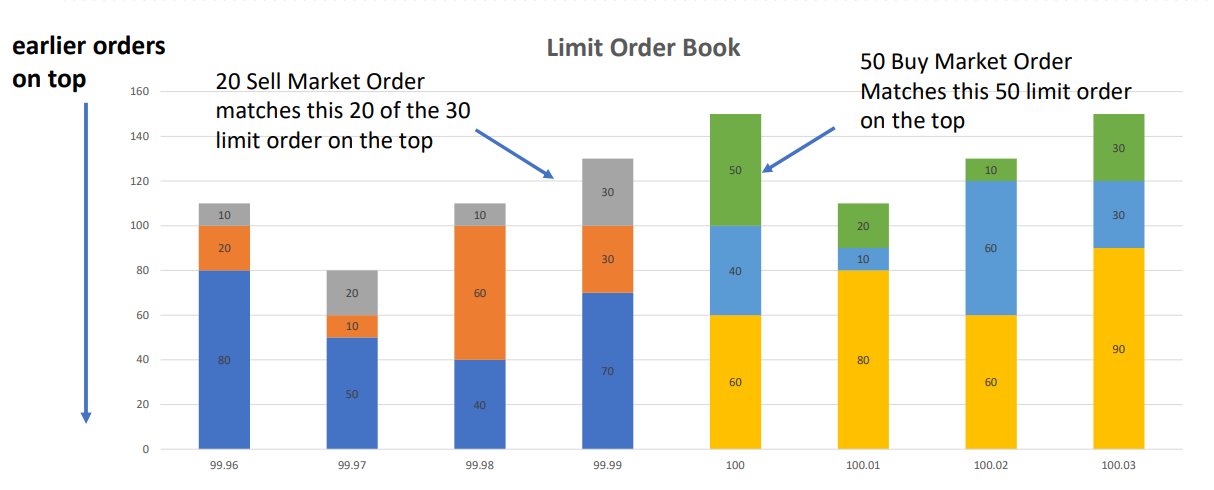
\includegraphics[scale=0.3]{img/limit_order_book.png}
    \end{center}

    The market makers profit off of the \textbf{bid-ask spread}, which is the difference in the buy and sell price. If a seller wants to sell at \$99.99 and a buyer wants to buy at \$100.00, then the market maker can buy the stock from the seller for \$99.99 and sell it to the buyer at \$100.00, making a \$0.01 profit. 

    We can also look at it from an economic perspective. We can draw the supply and demand curves for a certain company's stock. We can treat stocks as goods, with the company being the supplier and public investors as the consumers. 
    \begin{enumerate}
      \item The demand curve says: as the price for a stock, i.e. a piece of the company, increases the quantity demanded by the market (consumers) will decrease because the costs of buying the stock will outweigh the marginal value of the share. There is a very important distinction to make here between stocks and other type of goods. Unlike consumable goods which we can clearly observe a diminishing marginal value (drinking 1 can of soda vs 2 cans vs 3 cans vs...), stocks do not seem to have any diminishing marginal value. That is, if I buy 10 shares, I expect to get precisely 10 times the profit than if I bought just 1 share. The value is not diminishing, so why is the demand curve monotonically decreasing? That is because it is not diminishing \textit{for an individual}, but if we look at a market of many individuals, they all have different interpretations of what the marginal value of the stock is. Individual $A$ may interpret the marginal value as $\$10$, while $B$ sees it as worth $\$8$, and $C$ sees $\$6$. All three marginal utility curves would be horizontal, but if we take the market utility, we can see that it is decreasing (e.g. at the price of $\$7$, a share is attractive to $C$ but not $A, B$, and at $\$9$, a share is attractive to $B, C$ but not $A$). Buying an infinite number of shares is not realistic, so let us assume that each person has $\$25$ worth to invest. 
      \begin{center}
        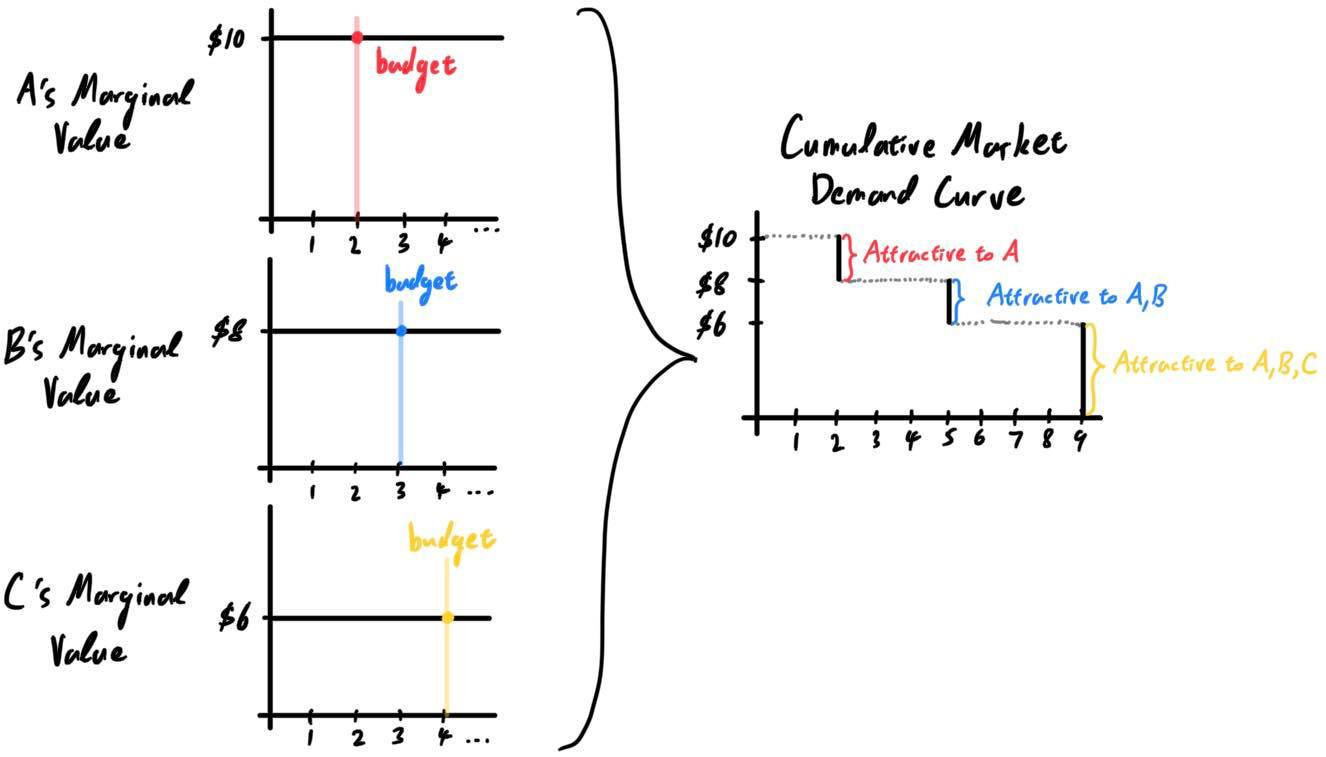
\includegraphics[width=0.8\textwidth]{img/Stock_demand_curve.jpg}
      \end{center}
      We can clearly see that the sum of these individual horizontal marginal value functions summed up produces a monotonically decreasing marginal value function and a monotonically decreasing demand curve for the total market. 

      \item The supply curve is simpler to interpret, since the only supplier is the issuing company (or whatever underwriting investment banks). By the law of supply, we can interpret that if the worth of the company's shares increases, then it would be logical for the company to issue more shares, all else being the same. This interpretation may be too oversimplistic, since we have to account for investor relations, dilution, and other factors, but it will do for now to justify that the supply curve of a stock is monotonically increasing.  
    \end{enumerate}

    Note that in general, the demand of a company's shares is much more volatile than the supply since there are many ways for the demand to shift, while few for the supply. The demand (not quantity demanded) of a company's shares can be changed from news, world events, production, and such, which occurs often and may even violently shift the outlook of the business. Unlike certain goods that are produced continuously, a company's floating shares will not change unless there is a new issuance or a private investors sells shares at market price. Therefore, supply (not quantity supplied) does not change easily. 

    Now, let us have the supply and demand curves of a company's share. Assume that it is at the equilibrium position, where $p^\ast_1$ is the current market price (bought and sold) and $q_1^\ast$ is the quantity demanded and supplied, as balance. 

    \begin{enumerate}
      \item If the demand increases, then the shift in the demand curve raises the equilibrium price to $p_2^*$, which raises the price of the stock. The quantity demanded/supplied also increases to $q_2^*$, but this desire to increase quantity cannot be met due to other factors. Therefore, we can interpret this case as such: The increase in demand can change the price accordingly, but the increase in desired quantity is offset by other factors (not being able to issue stocks freely). 
      \begin{center}
        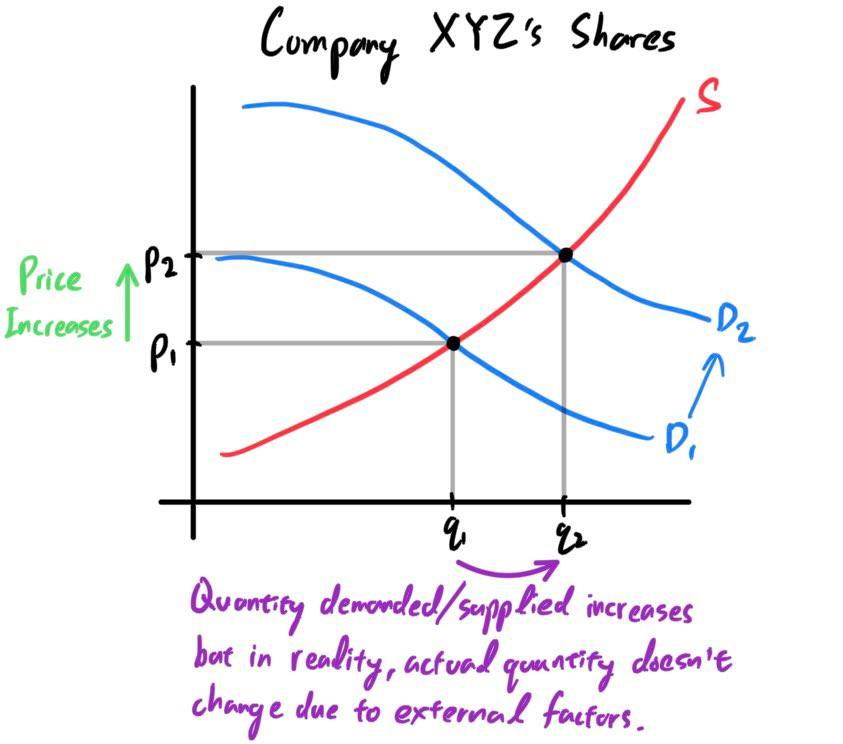
\includegraphics[width=0.4\textwidth]{img/Stock_Demand_Increase.jpg}
      \end{center}

      \item If the supply increases, then this is much simpler to explain. Due to dilution, one stock now represents ownership of a smaller portion of the company, driving the price down. The equilibrium (optimal) quantity demanded and supplied increases due to this higher supply, which is reflected in the reality that there are more more shares issued now. 
      \begin{center}
        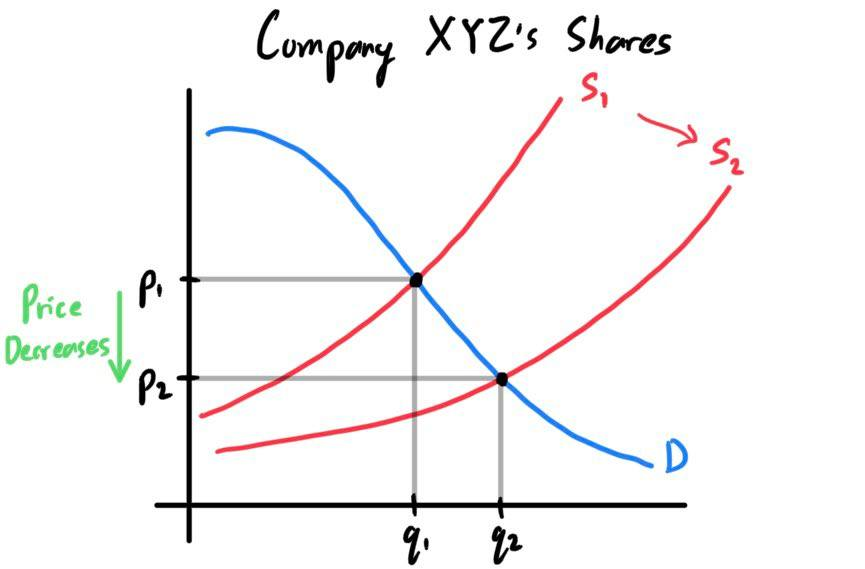
\includegraphics[width=0.4\textwidth]{img/Stock_Supply_Increase.jpg}
      \end{center}
    \end{enumerate}

  \subsection{Returns and Dividends}

    We can work out its return as the percentage increase or decrease of its price. But given that $X_t$ is close to $X_s$, we can look at the Taylor expansion of $\ln(X_t)$ to be 
    \begin{equation}
      \ln(X_t) \approx \ln(X_s) + \frac{1}{X_s} (X_t - X_s) \implies \frac{X_t - X_s}{X_s} \approx \ln (X_t) - \ln (X_s) = \ln \bigg( \frac{X_t}{X_s} \bigg)
    \end{equation}
    Therefore, we work with \textit{log returns} as an appropriate approximation of the return. As we will see later, the Black Scholes, which deals with continuous compounding interest rates, require lognormal as well. 

    \begin{definition}[Log Return]
      The \textbf{log return}, or \textbf{return}, of a stock from time $s$ to $t$ is defined 
      \begin{equation}
        R_{s, t} = \frac{X_t - X_s}{X_s} \approx \log\bigg( \frac{X_t}{X_s} \bigg) = \log(X_t) - \log(X_s)
      \end{equation}
      However, the return is almost always annualized, so we just write the return as $R$. 
    \end{definition}

    \begin{question}[Lognormal]
      This is because like a bunch of other stuff, we assume normal distributions. But it has specific flaws, which the lognormal fixes. 
    \end{question}

    \begin{definition}[Lognormal Distribution]
      
    \end{definition}

    It has its advantages: 
    \begin{enumerate}
      \item It is time-additive: If we have prices $X_r, X_s, X_t$ for $r < s < t$, we can see that 
      \begin{equation}
        R_{[i, j]} + R_{[j, k]} = \log \bigg(\frac{P_j}{P_i}\bigg) + \log \bigg( \frac{P_k}{P_j} \bigg) = \log \bigg(\frac{P_k}{P_i} \bigg) = R_{[i, k]}
      \end{equation}

      \item Symmetricity: It is well known that a stock going down $50\%$ and then going up $50\%$ does not return the stock to its original price, despite it "looking" like it did. This effect is killed when looking at log returns. If $X_t = X_s (1 - k)$ for $0 < k < 1$, then we know that it must scale up by a factor of $\frac{1}{1 - k} \neq 1 + k$ to get the original price. Indeed, it is clearly the case that 
      \[\log(1 - k) + \log(1 + k) = \log(1 - k^2) < 0\]
      and in fact is always less than $0$ (so we always lose money). This is due to the concavity of this function. 
      
      \item It focuses on relative change, which is typically invariant on the underlying price of the stock. 
    \end{enumerate}

    \begin{definition}[Dividend]
      Given time $s, t$ with $s < t$, the dividend that a stock $X$ pays within time interval $[s, t]$ is the random variable $D_{s, t}$
    \end{definition}

    \begin{definition}[Total Return]
      Given that you own stock $X$, the amount of money you would have made from time $s$ to $t$ is the random variable 
      \begin{equation}
        X_t - X_s + D_{s, t}
      \end{equation}
      The \textbf{total return} during that period is defined 
      \begin{equation}
        \mathbf{R}_{s, t} = \frac{X_t + D_{s, t} - X_s}{X_s} \approx \ln(X_t + D_{s, t}) - \ln (P_i)
      \end{equation}
      which is the price return plus the dividend rate. Again, the total return is almost always annualized.   
    \end{definition}

    These properties allow us to focus on the returns to calculate our metrics. 

    \begin{definition}[Expected Return]
      The \textbf{expected return} of a stock from time $s$ to $t$ is simply the expected value 
      \begin{equation}
        \mathbb{E}[R_{s, t}] = \mathbb{E} [ \log(X_t) - \log(X_s) ]
      \end{equation}
      where the expectation can be over the whole $\sigma$-algebra of sequences or can be conditioned on the two random variables $X_s, X_t$. The expected return over a year is $\mathbb{E}[R]$. 
    \end{definition}

  \subsection{Volatility}

    While we should be comfortable working with specific time periods $[s, t]$, most of the time we will be working with annualized statistics. Therefore, what we really just want to know is \textit{what kind of distribution is $R$ for a given stock?} It is also often (but probably incorrectly) assumed that $R$ just stays relatively the same random variable for a number of years. Therefore, everything boils down (for not) to accurately modeling $R$. The next best thing to do after the expectation is the second moment. 

    \begin{definition}[Volatility]
      The \textbf{volatility} of a stock is the standard deviation of $R$. 
      \begin{equation}
        \sigma = \sqrt{\mathrm{Var}[R]}
      \end{equation}
    \end{definition}

    \begin{definition}[Realized Volatility]
      Again, we don't know this actual value so we look at the next best thing: the sample volatility, known as the \textbf{realized volatility}. All realized volatility is again annualized, but the frequency and time periods that we look at it is important. 
      \begin{enumerate}
        \item The \textbf{historical (realized) volatility} takes into account the volatility of the past. 
        \item The \textbf{future realized volatility} is for the future. This is what everybody wants to know. 
      \end{enumerate}
    \end{definition}

    It seems that the most straightforward frequency and time for volatility is by taking all the yearly returns of every fiscal year up until now. This has the disadvantage of a small number of samples since most companies are publicly listed for at most a few dozen years.\footnote{Rather than taking samples $R_{0:365}, R_{366:730}, \ldots$, one might ask whether we can take $R_{0:365}, R_{1:366}, R_{2:367}, \ldots$. The answer is no, since these samples are correlated. } Therefore, people often resort to the following: 
    \begin{enumerate}
      \item 52-week volatility and scale it up by $\sqrt{52}$ to get the annual volatility.
      \item 250-day volatility and scale it up by $\sqrt{250}$ to get the annual volatility.\footnote{Traders often use $256$ since its square root is a clean $16$. }
      \item 12-month volatility and scale it up by $\sqrt{12}$ to get the annual volatility.
      \item Minutely volatility is not really used. 
    \end{enumerate}
    This is known as the \textbf{square-root-of-time rule}. It turns out that doing this is mainly for convenience and according to Natenberg, the time period and interval used for calculation does not affect the annual volatility much. 

    \begin{figure}[H]
      \centering 
      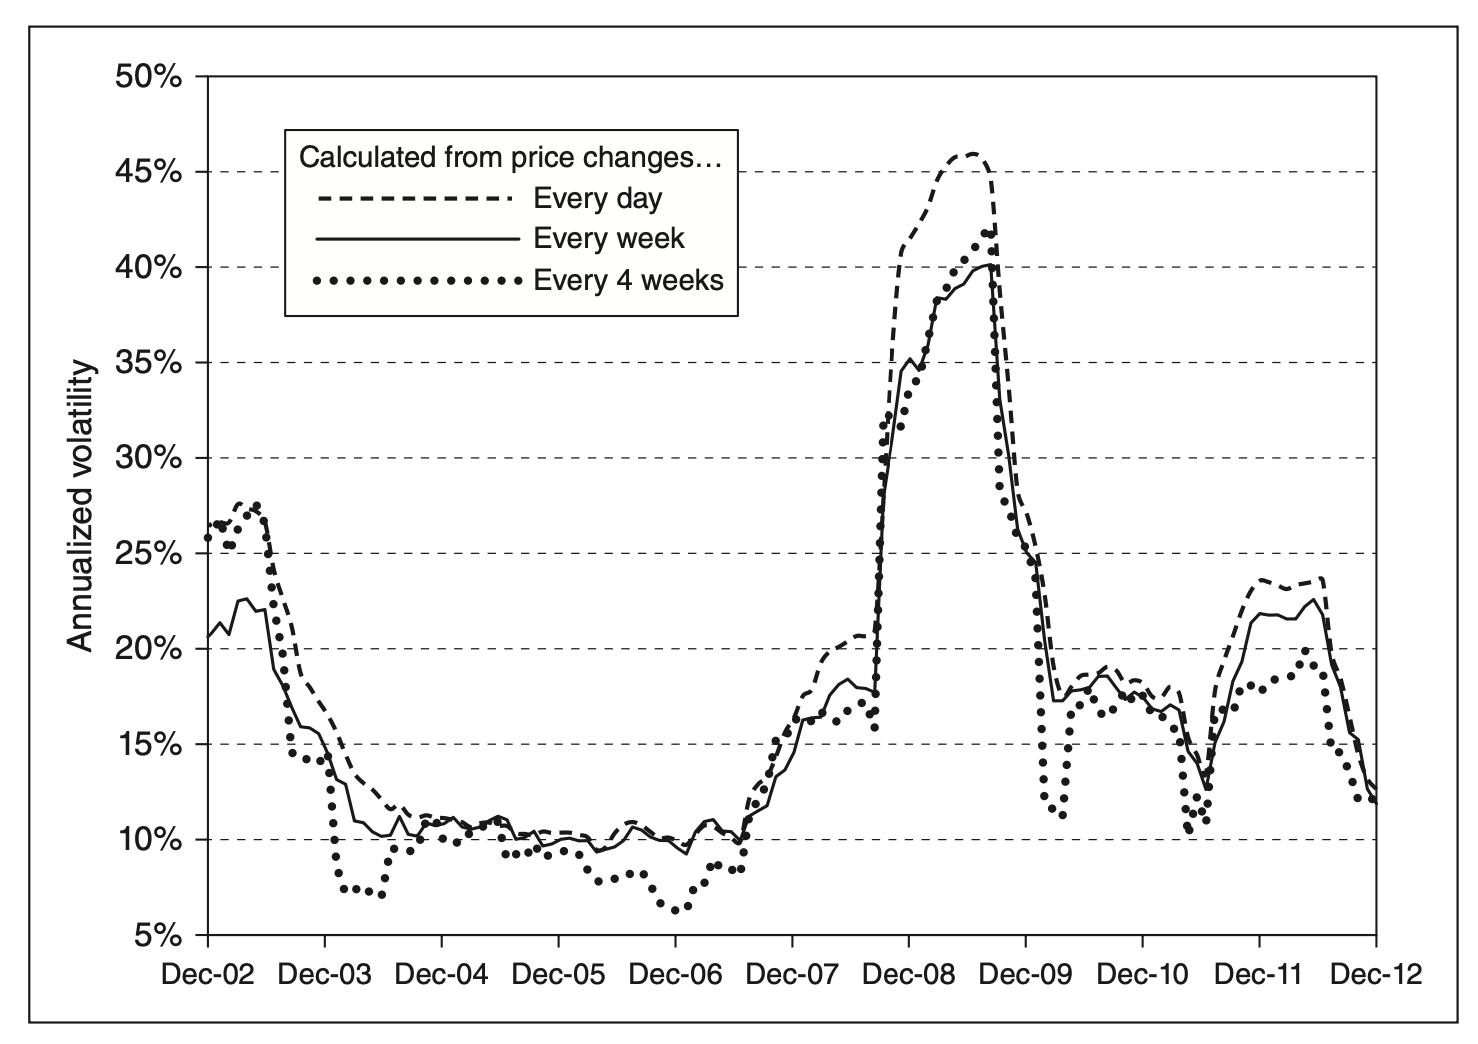
\includegraphics[scale=0.4]{img/vol_time_periods.png}
      \caption{The three intervals used to calculated a 250-day volatility. While a stock may have wild daily fluctuations that cancel out over each week, but is an exception. For the vast majority of stocks, vast daily fluctuations indicate vast weekly, monthly, etc. fluctuations. } 
      \label{fig:vol_with_time}
    \end{figure}
  
  \subsection{Interest Rates}

    \begin{definition}[Zero Coupon Bonds]
      A convenient way to measure interest rates are through \textit{zero-coupon bonds}, which do not pay coupon payments but are instead issued at a discount to their par value. Upon maturity, it pays the bondholder in full face value (e.g. U.S. treasury bills). 
    \end{definition}

    This means that the value of a ZCB is precisely determined only by the interest rate $r$. Therefore, we define the value of a ZCB as follows. 

    \begin{definition}[ZCB]
      A ZCB with maturity $T$ that pays $1$ has a value of 
      \begin{equation}
        Z_r (t, T) 
      \end{equation}
      where the $r$ may be omitted if the rate is assumed to be known or not calculated yet. Depending on how we model it, it may be treated as 
      \begin{enumerate}
        \item discrete, where 
          \begin{equation}
            Z_r (t, T) = (1 + r)^{T - t}
          \end{equation}
        \item continuous, where 
          \begin{equation}
            Z_r (t, T) = e^{- r (T - t)}
          \end{equation}
      \end{enumerate}
    \end{definition}

    While we won't directly work with ZCBs as much, the following provides a very convenient notation to determine prices. 

    \begin{example}[Basic ZCB Application]
      Given that you will receive \$100 in time $T$, the present value of this future cash flow is 
      \begin{equation}
        100 \cdot Z(t, T)
      \end{equation}
      If you have the decision to receive $X$ dollars today or $Y$ dollars in 1 year, then we can take the future cash flow $Y$ and discount it to today and compare them. We should therefore accept $Y$ in 1 year iff 
      \begin{equation}
        Y \cdot Z(t, t + 1) > X  
      \end{equation}
      Therefore, to calculate the present value of some future cash flow, just multiply it by $Z$. If you want to take some present cash flow and forward it into the future, then divide it. 
    \end{example}

  \subsection{Measures}

    While the expected returns are important, the concept of \textbf{risk} is equally if not more. This is a slippery term, used to mean different things, but it is essentially some characterization of the distribution of the returns. The variance, or standard deviation, of $R$ was one form of risk, but there are other ones that we will introduce here. 

    \begin{definition}[Sharpe Ratio]
      The \textbf{Sharpe ratio} is a measurement of risk-adjusted annual return. Given that you have some stock price with total return $R$ and volatility $\sigma$, the Sharpe ratio is defined as the random variable
      \begin{equation}
        S = \frac{R - R_f}{\sigma}
      \end{equation}
      where $R_f$ is risk-free return (e.g. the return you earn on U.S. Treasury bonds), which can be considered as a constant random variable. Sometimes, $R_f$ may not be constant and may be some time-series data itself. 
    \end{definition}

    Another property we would like to investigate is perhaps some tail bounds. 

    \begin{definition}[Value at Risk]
      The \textbf{value at risk (VaR)} over a time horizon of $T$ at $p \in [0, 1]$ is 
      \begin{equation}
        \Phi^{-1}(p)
      \end{equation}
      which tells us the loss we could incur by the end of $T$ with a probability of $p$, where $\Phi()$ is the CDF of $R_{0, T}$. $p$ is usually taken to be 1\% or 5\%. 
    \end{definition}

\section{Secondary Markets}

  \subsection{Types of Stock Orders}

    \begin{definition}[Stock Orders]
      The two most common orders one can do is the market order and the limit order. 
      \begin{enumerate}
        \item A \textbf{market order} just buys or sells securities at the market price. This ensures that the transaction will be completed, but the price at which you buy or sell may not be what you want. 
        \item A \textbf{limit order} buys or sells at least at a certain price. It ensures that you get the price you want for a transaction, but it may not be carried out always. 
        \begin{enumerate}
          \item A buy limit order at \$X tells the broker to buy a stock at \$X or lower. 
          \item A sell limit order at \$x tells the broker to sell a stock at \$ or higher. 
        \end{enumerate}
        \item A \textbf{stop loss order} is used to limit an individual's loss or lock in a profit on a stock position. 
        \begin{enumerate}
          \item If an investor buys a stock at \$100, they can make a stop loss at \$95. This means that when the stock price reaches \$95, then it will automatically place a market order to sell the stock (the price may not be fulfilled at exactly \$95 due to volatility). 
          \item If an investor has a short position, on the stock, then they can put a stop loss order at \$105, essentially telling the broker to buy the stock when the price reaches \$105. 
        \end{enumerate}
      \end{enumerate}
    \end{definition}

    \subsubsection{Short Selling}

      In addition to holding a long position, we can \textbf{short sell}, or short, a stock. Given that 100 shares of AAPL are each priced at \$100, we can borrow shares from some investor (probably an institutional investor), sell it on the market for \$100, and hope for the price to drop so we can buy it back. This is pretty symmetric to longing a stock, and many hedge funds use a \textbf{long-short equity strategy} involving a combination of longs and shorts, but there are additional risks. 
      \begin{enumerate}
        \item You must pay additional interest for borrowing stocks. 

        \item Your potential losses is not bounded. 

        \item If you have too much unrealized losses as the stock price goes up, then you may not have enough \textbf{margin} (cash) in your account to even buy back to stock. To prevent this, your broker may issue a \textbf{margin call}, which forces you to buy the stocks back, locking in your loss, unless you add more capital to your account. This margin call may not happen right at the point when your free cash is not enough to buy back all shorted shares. Rather, your brokerage may run some complicated statistical simulations, calculate some confidence interval, and then decide on a threshold that determines whether you will get a margin call. 
      \end{enumerate}
      The third risk is the deadliest, and at worst, you can get \textbf{short-squeezed}. Let's explain how this works. Say you and a bunch of other investors shorted GME. GME prices start going up, and it reaches a point where some investors have to buy back the GME shares due to a margin call. The investors buy back the GME at market price, which adds more orders to the limit order book, causing the price to go even higher. This higher price causes more short-sellers to buy back GME due to additional margin calls, causing GME to go even higher, and so on. This positive feedback loop is extremely deadly, killing off many short sellers. 

      Sometimes, the ethics of short selling are called into question. People who want to ban shorting state that short selling can drive down the stock price, which can be bad because it doesn’t spur the economy and reduces optimism in stock markets. Short selling means that stock is being borrowed and sold on the market, increasing supply, and therefore (all else being equal) decreasing price. However, these short sellers keep the stock price more in line with reality, and bad companies are punished by short sellers. 

      Finally, the entities that drive this short selling are \textbf{prime brokers}, which are large financial institutions (usually investment banks) that provide financial management to mainly hedge funds. They act on behalf of the short seller, locating the assets to be sold short for them and providing them with a margin account (which must hold capital to the sum of at least 150\% of the value of the initial transaction). They enable hedge funds to borrow large amounts of stocks from institutional investors to short-sell them and allow them to access large amounts of margin from commercial banks. The prime brokerage makes money through commissions. Prime brokers can also loan capital to investors to increase their leverage, and they also provide financial research and analytics to their clients. 

  \subsection{Counterparties and Clearing Houses}

    Trader, Broker, Liquidity provider, Market maker 

    NYSE is a stock exchange that leases a space to different market makers (banks, hedge funds). It also makes money thorugh fees from companies to be listed on NYSE. If a crash happens (i.e. a market maker buys a stock and it tanks before they can sell it), then the market makers get screwed. 

    Think about when one party buys stocks or bonds. Their downside is limited to the amount they paid on the stock, but there are many other cases where they may not be protected. 

    \begin{example}[Risks Associated with Trades]
      \begin{enumerate}
        \item The simplest case is when they are in debt. They want to borrow $X$ for a certain time, and repay it back in a year at some interest rate $X (1 + r)$. However, they may not have the money by then. 
        \item When they short a stock, they can borrow money from another party that owns the stock, sell it, and buy it back at a lower price. However, if the price of the stock rises, then they must pay even more money to buy it back, and they may not have enough money to. 
        \item When they buy a stock on margin, they borrow money from a broker to buy the stock, and they must pay back the broker with interest. However, the price of the stock may fall and the borrower, even after liquidating the stock, may not have enough money to pay back the broker.
        \item Someone who longs a forward contract may not have enough money to pay the difference between the forward price and the spot price.
      \end{enumerate}
    \end{example}

    \begin{definition}[Counterparty]
      A \textbf{counterparty} is the other party in a financial transaction. \textbf{Counterparty risk} is the likelihood or probability that one of those involved in a transaction might default on its contractual obligation. It can exist in credit, investment, and trading transactions.\footnote{This is formalized through creditworthiness, which takes many forms such as bond ratings, corporate credit ratings, and FICO scores.}
    \end{definition}

    Note that in a vanilla exchange, the two parties trading are counterparties to each other. This is called a \textbf{bilaterial exchange}. As we have seen, this is risky since if one party defaults, the other party is left with nothing. Therefore, the markets introduce a middleman that takes care of this risk. 

    \begin{definition}[Clearing House]
      The \textbf{clearing house} is an entity that is counterparty to all parties. This means that if party A and party B want to trade, they must go through the clearing house. The clearing house buys from B and sells to A. Therefore, the counterparty risk is now within the clearing house.
    \end{definition}

    It seems that we have simply moved the risk from the traders to the clearinghouse, and this is correct. The traders are glad that the risk is gone from them since they will always be paid by the clearinghouse, and the clearinghouse can add additional regulations on trading to reduce the risk of default. The first regulation they should impose are \textit{capital requirements}.\footnote{This is slightly different from margin. We will get to margin later. } 

    \begin{definition}[Capital]
      \textbf{Margin} is simply cash or some other asset (stocks, bonds, etc.) that can be used as collateral during a trade. Note that this does not mean that the collateral must be invested into anything. It is just restricted to sit there in your bank account. 
      \begin{enumerate}
        \item Cash is the most liquid form of margin, and is the most common form of margin. 
        \item Bonds are also a common form of margin, and Treasury bonds are usually valued at 90\% of their market value.
        \item Stocks are also a common form of margin, and are usually valued at 50\% of their market value. 
      \end{enumerate}
    \end{definition}

    Therefore, the cost of going into the trade is not just the trade itself, but also the capital requirements. These requirements are generally very inflexible unless you have a good relationship with your broker and are a big trader. 

  \subsection{Brokers}

    Brokers are the middlemen between the traders and the exchanges. They are the ones that execute the trades on behalf of the traders. They are also the ones that provide the traders with the margin. 

    \begin{definition}[Broker]
      A \textbf{broker} is a person or firm that executes orders on behalf of a trader. They are the ones that provide the traders with the margin. 
    \end{definition}

    Brokers can be classified into two types: 
    \begin{enumerate}
      \item \textbf{Full-service brokers} provide a large suite of services to their clients, including research and advice. They are usually more expensive than discount brokers. 
      \item \textbf{Discount brokers} are cheaper than full-service brokers, but they do not provide as many services. They are usually used by more experienced traders. 
    \end{enumerate}

    \begin{example}[Famous Brokers]
      The following are famous brokerage firms: 
      \begin{enumerate}
        \item Robinhood 
        \item Charles Schwab 
        \item Interactive Brokers
        \item Fidelity
      \end{enumerate}
    \end{example}

  \subsection{Market Makers and Liquidity Providers}

    They quote a bid ask price and provide liquidity to the market. The buyers and sellers like us (retail, institutional, etc.) are market takers. 

    \begin{example}[Market Makers]
      Here are some famous market makers. 
      \begin{enumerate}
        \item Akuna
        \item Jane Street 
        \item Citadel 
        \item Optiver 
      \end{enumerate}
    \end{example}

  \subsection{Exchanges}

  \subsection{OTC Markets and Dark Pools}

    The inefficient aspect about markets that they are sensitive to large \textbf{block trades}, which are defined to be a trader involving at least 10,000 shares or at least \$200,000 (though they can get much larger). They are usually made by institutional investors and are often privately negotiated in order to prevent market price changes and fluctuations. When an institutional investor would like to make a sell block trade, they can either 

    \begin{enumerate}
      \item sell it on the exchange, where it will cause downwards pressure on the price, causing \textbf{slippage} (think of the limit order book: this sell order would clear out all buy orders past the sell price) and perhaps affecting the wider market. Even worse, once an order to sell a huge block has been filled, an investor can submit a buy order at a lower price in hopes that the block sell will hit his lowered price (this is an example of front running). 

      \item sell it privately off an exchange, but finding other parties to buy such a large amount is difficult. 
    \end{enumerate}

    Either way is quite unfavorable. The market impact of a sale of one million shares in Company XYZ could still be sizable regardless of which option the investor chose since it was not possible to keep the identity or intention of the investor secret in a stock exchange transaction. 

    These investors can trade in \textbf{dark pools}, which are privately organized financial exchanges for trading securities, also an \textbf{alternative trading system} (ATS). They were created originally to facilitate block trading by institutional investors who did not wish to impact the markets with their large orders. Most importantly, they keep trades anonymous. They allow traders to make block trades without having to publicize who they are, the buy/sell price, or the number of shares traded. 

  \subsection{Exchange vs OTC Markets}

    In a trading floor or pit, there are groups of traders huddled at certain physical locations that trade a certain asset, like corn futures. Back then, there would be individual traders that have their own small capital that they can trade with, called \textbf{locals}, but they have been dominated by traders that work for large financial institutions, causing locals to be either pushed our or joined with the firms. Market making firms like Akuna have pit traders, who have headsets and tablets, that are in real-time communication with the screen traders upstairs. 

    Standing in the perimeter of the trader circle are the \textbf{brokers}, who relay orders between the traders in the pit and outside of the pit. These brokers also have devices that allow them to communicate with \textbf{off floor} parties, who are individuals that are interested in these products. 

    \begin{example}[Off Floor Parties]
      Some examples of off floor parties are: 
      \begin{enumerate}
        \item Hedge funds, who have devised trading strategies that they want to implement, e.g. using drones to look at the harvest quantity. Now they want to gain exposure to the corn market. 
        \item Banks might also want to use client money to develop a trading strategy. 
        \item Consumers such as Kellogs (which needs a lot of corn to make cereal) might be interested in buying contracts to hedge their underlying exposure. 
        \item Producers like corn farmers might want to buy some contract to lock in the price in which they can sell it at. 
        \item Large funds like pension funds or family money. 
        \item Retail investors like small, non-professional traders that might dabble in options.  
        \item Other market makers might be connected to these brokers
      \end{enumerate}
    \end{example}

    Now if some off floor party decides to sell some calls, they will call their broker and ask to quote some prices. This means that they are asking for bid and offer prices. These traders might quote the following prices: 

    When more people want to buy and sell things, they must go to an \textbf{exchange}, which is literally a physical space that is leased to various parties (e.g. large banks, hedge funds) so that they can exchange goods. These exchanges also collect money through fees from companies to be listed on NYSE. There are two big exchanges, the NYSE and the NASDAQ, in the U.S., both located in New York. 

    Us retail traders are not direct participants of the exchange; the parties that participate there are called the \textbf{market makers}, or \textbf{liquidity providers}. Market makers, usually large banks or financial institutions (like hedge funds), make sure that there is enough trading volume to ensure liquidity in the market. A buyer and a seller must meet together to complete a deal, and to ensure that this happens smoothly (i.e. provides liquidity), a market maker buys stocks (through the individual's brokerage) and sells them to the corresponding recipient. Essentially, they provide a pool of shares and act as intermediaries between them. They profit from the bid-ask spread, though sudden volatility is always a risk. For example, if a crash happens (i.e. a market maker buys a stock and it tanks before they can sell it), then the market makers get screwed because they are left with an undervalued stock. 

    The trader cannot directly trade through the market makers. They must contact their \textbf{broker}, which is another company that acts as an intermediary. If I want to buy a stock, my buy order gets sent to my broker, which gets sent to the market makers, which pairs me up with a seller through their own broker, and the transaction is completed. These brokers make money through commissions from the traders and from trading in dark pools, which we'll talk about later. They also give access to traders the forecasts of analyst reports for companies and other research. 

    \begin{center}
      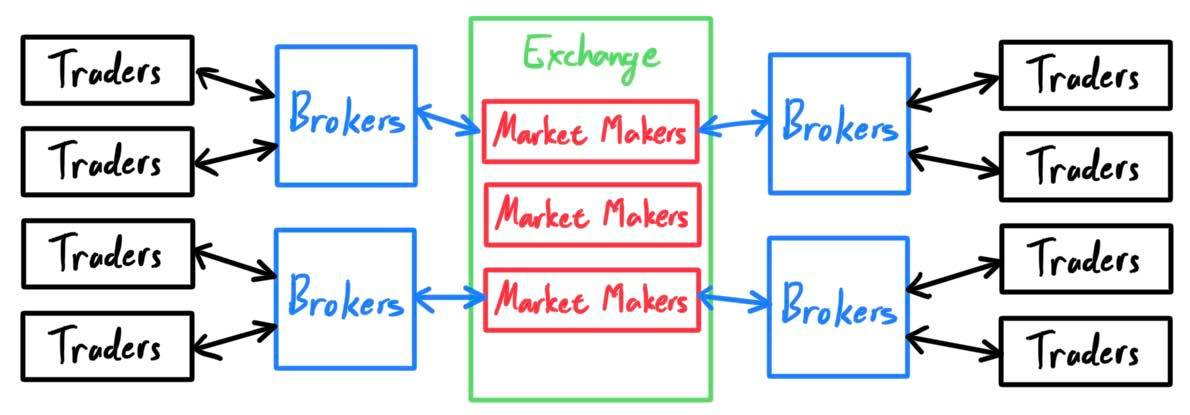
\includegraphics[scale=0.3]{img/exchange.jpg}
    \end{center}

    Clearly, there can be some shady stuff going on here, but luckily, the SEC and the FINRA consistently regulate the markets to ensure fairness for the little players (retail investors). One of the most important regulations is the 2005 Regulation NMS (National Market System), which required exchanges to publish the best bid and offer price for each stock, required them to route orders to the trading venue with the best price, and had set the minimal price quotation increment to \$0.01. This ensured transparency and protection of the investor with the best price execution (but this can be taken advantage of by high frequency traders). 

    \begin{definition}[Exchange Markets]
      \textbf{Exchange markets} are markets that exchange \textit{standardized} contracts and is \textit{highly regulated} (to protect investors) by a central authority. A buyer and seller come together to trade a contract, and they enter the contract through a \textbf{clearing house}, which is the \textit{counterparty} to all trades. That is, both the buyer and seller enter into a contract with the clearing house. Doing this reduces the counterparty risk by ensuring that both sides have adequate \textit{margin}. For example, if the buyer wins the bet and the seller can't pay, the clearing house will pay the buyer.
    \end{definition}

    \begin{question}
      Talk about counterparties, clearinghouses. 
    \end{question}

    \subsubsection{Market Making and High Frequency Trading}

      A significant mover of markets are \textbf{high frequency traders}, or HFTs. HFT is a type of algorithmic trading that are characterized by high speeds and high turnover rates. It is the primary type of algorithmic trading and consists of about 50\% of all equity trades in the U.S. There is an average of about 1 trader per 10 milliseconds. Whether HFT is beneficial is very controversial: 
      \begin{enumerate}
          \item Some argue that it is good since it increases liquidity and lowers transaction costs for retail investors. Even for potentially risky stocks (e.g. very overvalued), HFTs will always make a market out of them. 
          \item It can be considered unfair because it gives a huge advantage to HFT firms through front-running and other short-term strategies. This also increases the probability of \textbf{flash-crashes} (e.g. 2010 flash crash). 
      \end{enumerate}
      Unsurprisingly, many HFT firms are market makers due to their ability to provide liquidity. 

      The primary form of HFT is \textbf{scalping}, which profits off of small price changes. The multiple benefits and drawbacks are easy to spot: 
      \begin{enumerate}
          \item It requires a strict exit strategy since one large loss could eliminate the many small gains the trader worked to obtain. 
          \item It also requires a much higher ratio of winning trades vs losing ones, while keeping profits roughly equal or slightly bigger than losses. 
          \item A brief exposure to the market diminishes the probability of running into an adverse event like a crash. 
          \item Smaller moves are easier to obtain, so there are plenty of opportunities to exploit. 
      \end{enumerate}
      This strategy is extremely sensitive that even the physical location of the firm relative to the exchange matters. Heavy money in infrastructure is invested. 


    \begin{definition}[OTC Markets]
      In \textbf{over the counter markets} (OTC), there is also an interaction between the buyer and the seller, but it is done in two ways. 
      \begin{enumerate}
        \item In \textit{bilateral clearing}, the buyer and seller are the counterparties to each other, and so there is indeed the risk of default on one side. 
        \item Post-2008, there has been a push to clear through a \textit{central counterparty}. Therefore, there has been a slow push to clear OTC derivative trading to reduce this counterparty risk. 
      \end{enumerate}
      Finally, the OTC market is much larger (about 5 to 10 times larger in terms of the principal dollars underlying the assets) than the exchange and is less regulated since most of the players are institutional investors (they don't need as much protection but need more flexibility).  
    \end{definition}

\section{Momentum Strategies}

  Momentum strategies can be divided into \textbf{momentum trending}, which bets that the stock price will continue following the trend, and \textbf{momentum reversing}, which bets that the stock price will revert back to some mean. 

  \subsection{Moving Averages}

    The simple moving average and the exponential moving averages represent where the stock's price is at average. 

    \begin{definition}[Simple Moving Average]
      Let us have some stock price $\{P_i\}_{i=0}^N$ and fix some lookback parameter $L$. Then, the $L$-period \textbf{simple moving average (SMA)} of the stock is the average of prices of the past $L$ periods, $\{S_i\}_{i=L-1}^N$, where 
      \[S_i = \frac{1}{L} \sum_{j=i-L + 1}^i P_j\]
    \end{definition}

    \begin{definition}[Exponential Moving Average]

    \end{definition}

    We can build momentum strategies by comparing two different MAs of lookback periods $L_1 < L_2$. We can compare the current price to the moving averages, but the current price can be thought of as the $1$-period moving average anyways. The $L_2$-MA is thought of as the long term trend of the stock, while he $L_1$-MA is the short-term trend. The follow are essentially MA strategies. 
    \begin{enumerate}
        \item Momentum Trending: 
        \begin{enumerate}
            \item If the $L_1$-MA is above the $L_2$-MA, then the stock has momentum upwards. $\implies$ Long. 
            \item If $L_1$-MA is below the $L_2$-MA, then the stock has momentum downwards. $\implies$ Short. 
        \end{enumerate}
        
        \item Momentum Reversing: 
        \begin{enumerate}
            \item If the $L_1$-MA is above the $L_2$-MA, then the stock has momentum upwards. $\implies$ Short. 
            \item If $L_1$-MA is below the $L_2$-MA, then the stock has momentum downwards. $\implies$ Long. 
        \end{enumerate}
    \end{enumerate}

  \subsection{Bollinger Bands}

    \begin{definition}[Bollinger Bands]
      Let us have some stock price $\{P_i\}_{i=0}^N$ and fix some lookback parameter $L$, along with some $z$-score $Z$. We compute the standard deviation of the prices $P_i$ in the past $L$ periods to get $\{\sigma_i\}_{i=L-1}^N$. 
      \begin{enumerate}
        \item The \textbf{middle band} is defined to be the $L$-period SMA, which we will call 
        \[\{\mathcal{M}_i\}_{i=L-1}^N\] 
        \item The \textbf{upper band} is defined to be the band that is $Z$ standard deviations above the middle band. 
        \[\{\mathcal{U}_i\}_{i=L-1}^N = \{M_i + Z \sigma_i\}_{i=L-1}^N\]
        \item The \textbf{upper band} is defined to be the band that is $Z$ standard deviations below the middle band. 
        \[\{\mathcal{L}_i\}_{i=L-1}^N = \{M_i - Z \sigma_i\}_{i=L-1}^N\]
      \end{enumerate}
    \end{definition}

    Now the algorithm for Bollinger bands is very simple. 
    \begin{enumerate}
      \item In a momentum following case, if $P_i$ crosses below $\mathcal{L}_i$, we short, and if $P_i$ crosses above $\mathcal{U}_i$, we long. 

      \item In a momentum reversing case, if $P_i$ crosses below $\mathcal{L}_i$, we long, and if $P_i$ crosses above $\mathcal{U}_i$, we short. The upper band acts as a resistance level, and the lower band acts as a support level. 
    \end{enumerate}

  \subsection{Relative Strength Index}

    The relative strength index indicates the momentum or lack of it. 

    \begin{definition}[Relative Strength Index]
      Let us have some stock price $\{P_i\}_{i=0}^N$. Let us define the period changes as $\{D_i\}_{i=1}^N$ with $D_i = P_i - P_{i-1}$. Then, the total gain and total loss can be defined as 
      \[D_\mathrm{gain} = \sum_{D_i > 0} |P_i - P_{i-1}|, \;\;\; D_{\mathrm{loss}} = \sum_{D_i < 0} |P_i - P_{i-1}|\]
      Then, the \textbf{relative strength index (RSI)} is defined to be 
      \[RSI = 100 \, \frac{D_{\mathrm{gain}}}{D_\mathrm{gain} + D_{\mathrm{loss}}}\]
      which ranges in $[0, 100]$, where $0$ is extremely bearish and $100$ is extremely bullish. Roughly, the RSI being $30$ means that for every 1 increase in a period, there are 2 decreases in other periods. The RSI being $70$ means that for every 1 decrease, there are 2 increases. 
    \end{definition}

    The algorithm is quite simple: 
    \begin{enumerate}
      \item In a momentum following case, if the RSI is below $30$, we short, and if the RSI is above $70$, we long. 
      \item In a momentum reversing case, if the RSI is below $30$, we long, and if the RSI is above $70$, we short. 
    \end{enumerate}

  \subsection{Determining Momentum Trending or Reversing}

    Now how can we quantitatively decide whether we should use a momentum trending or reverting strategy? We can measure this behavior of a stock by looking at its autocorrelation. 

    \begin{definition}[Autocorrelation]
      Let us have some stock price $\{P_i\}_{i=0}^N$ and fix some lookback parameter $L$. We construct a lagged version $\{P_i\}_{i=0}^{N-L}$ and compute the correlation of this lagged time series with the original. 
      \[\mathrm{Corr}(\{P_i\}_{i=0}^{N-L}, \{P_i\}_{i = L}^{N})\]
      is called the $L$-period \textbf{autocorrelation} of the stock price. 
    \end{definition}

    We can determine which strategy to use as follows. Let us assume that $L$ is small.  
    \begin{enumerate}
      \item If this autocorrelation is high (near $1$), then this indicates that if the stock moves in a certain direction, it is likely to move in that same direction $L$ periods later. So we should use a momentum following strategy. 
      \item If it is negative (near $-1$), it indicates that if the stock moves in a certain direction, it is likely to move in the opposite direction $L$ periods later. So we should use a momentum reverting strategy. 
    \end{enumerate}
    Trend following stocks tend to be growth stocks, while trend reversing ones are the traditional conservative companies. 

\section{Statistical Arbitrage}

  Intuitively, pairs trading takes two stocks of very similar companies and bets that they will rise and fall together. If one rises and the other falls, then we can long the one that falls and short the one that rises, ultimately betting on the way that they will converge. Let's first look at an intuitive examples with temperature betting. 

  \begin{example}[Temperatrue Arbitrage]
    Say you are given the following trades:
    \begin{enumerate}
      \item 65 at 66 on the temperature of San Francisco, $S$
      \item 45 at 47 on the temperature in Kyiv, denoted $K$
      \item 25 at 26 on the temperature of San Francisco minus Kyiv, $S - K$ 
    \end{enumerate}
    What do you do? Let's compare these markets. You see that buying $K$ and $S - K$, which you can do for $47 + 26 = 73$ must be the same as buying $S$ alone, which is $66$. Therefore there is a price mismatch. You should therefore long $S$, short $K$, and short $S - K$. 
  \end{example}

  To do this, take two sets of stock prices $P_t$ and $Q_t$ and model them with the assumption that the log returns are linearly correlated by the following relationship.\footnote{What beginners assume is that if $P$ rises by $5\%$, then $Q$ will also rise by $5\%$. But what if companies $P$ and $Q$, who use the same supply chains, exist such that $P$ is, say twice as dependent as $Q$? Then, if $P$ goes down by $5\%$, then $Q$ may go down by $2.5\%$, and our assumption should be that it is \textit{linearly correlated}. }
  \begin{equation}
    \frac{\Delta P}{P} = \beta \frac{\Delta Q}{Q} \iff \log(P_j) - \log(P_i) = \beta \big( \log(Q_j) - \log(Q_i) \big)
  \end{equation}

  This results in the model 
  \begin{equation}
    \log(P) = \beta \log(Q) + \alpha + \epsilon
  \end{equation}
  which can be seen to be equivalent because taking the change over time $[i, j]$ on both sides gives 
  \begin{equation}
    \Delta \log(P) = \beta \Delta \log(Q) + \Delta \epsilon \iff \frac{\Delta P}{P} = \beta \frac{\Delta Q}{Q} + \Delta\epsilon 
  \end{equation}
  So, if we look at
  \begin{equation}
    \{\epsilon_i\}_{i=0}^n = \{\log(P_i) - \beta \log(Q_i) - \alpha\}_{i=0}^n 
  \end{equation}
  we expect this to be a $0$-mean time series. Let the standard deviation be $\sigma = \sigma(\{\epsilon_i\}_{i=0}^n)$ and let us fix some $Z$-score threshhold. Then 
  \begin{enumerate}
    \item If $\epsilon_i > Z \sigma$, then short $P$ and long $Q$. 
    \item If $\epsilon_i < -Z \sigma$, then long $P$ and short $Q$. 
  \end{enumerate}

  \subsection{Long/Short Market Weights}

    But how much should we long or short? Let's look at a couple scenarios: 
    \begin{enumerate}
        \item If $\beta = 1$, and we shorted $\$99$ of $P$ and long $\$1$ of $Q$, then a $5\%$ rise in $P$ would result in $5\%$ rise in $Q$, but since we shorted much more of $P$, we would have a net loss. To mitigate this risk, we should have a weight of $P:Q = 1:1$. 
        \item If $\beta = 10$, and we shorted equally $\$50$ of $P$ and long $\$50$ of $Q$, then a $10\%$ rise in $P$ would result in a $1\%$ rise in $Q$. But since we had equal weights in $P$ and $Q$, this scenario would cause 10 times more losses in $P$ than gains in $Q$, resulting in a net loss. To mitigate this risk, we should have a weight $P:Q = 1:10$. 
    \end{enumerate}
    So, we need to be careful of setting the ratio of our market weights of the stocks $P$ and $Q$: 
    \[\lambda = \frac{\MV_Q}{\MV_P}\]
    Intuitively, we can see that our ratio should be $1: \lambda = 1:\beta$, i.e. $\lambda = \beta$, but let's formalize this with some mathematical derivation. Our portfolio value is 
    \[V = \MV_P + \MV_Q\]
    where $\MV_P = n_P P$ and $\MV_Q = n_Q Q$, where $n_P, n_Q$ are the number of shares of $P, Q$. If we are longing $P$ and shorting $Q$, then $n_P > 0$ and $n_Q < 0$. Then, our change in portfolio value $V$ is 
    \begin{align*}
        \Delta \V & = \Delta \MV_P + \Delta \MV_Q \\
        & = \MV_P \bigg[\frac{\Delta \MV_P}{\MV_P} + \frac{\MV_Q}{\MV_P} \frac{\Delta \MV_Q}{\MV_Q}  \bigg] \\
        & = \MV_P \bigg[ \frac{\Delta P}{P} + \lambda \frac{\Delta Q}{Q} \bigg] \\
        & = \MV_P \bigg[ \beta \frac{\Delta Q}{Q} + \Delta \epsilon + \lambda \frac{\Delta Q}{Q} \bigg] \\
        & = \MV_P \bigg[ (\beta + \lambda) \frac{\Delta Q}{Q} + \Delta \epsilon \bigg] 
    \end{align*}
    Therefore, our change in portfolio value depends on the terms in the last equation. We don't want the change $\Delta Q$ to have any effect on the performance, so we set $\lambda = - \beta$, ultimately resulting in 
    \[\Delta \V = \MV_P \Delta \epsilon\]
    and now our performance is purely dependent on $\Delta \epsilon$. We would like $\Delta \V$ to be positive, so if we are longing $P$, i.e. $\MV_P > 0$, then we want $\Delta \epsilon$ to also be positive. Likewise, if we are shorting $P$, then $\MV_P < 0$ and so we want $\Delta \epsilon < 0$. 

  \subsection{Choosing Correct Stocks}

    So, how do we ensure that $\Delta \epsilon$ behaves this way? Remember that $\{\epsilon_i\}$ is $0$-mean time series. However, we want to impose the additional condition that it is \textit{mean-reverting} as well. That is, we don't want it to diverge or oscillate too frequently $\epsilon_i$, since if it did then there is the risk of $\{\log(P_i) - \beta \log(Q_i) - \alpha\}_{i=0}^n$ swinging too widely, resulting in losses. In other words, if $\epsilon_i > 0$, then we want $\Delta \epsilon_{i + 1} = \epsilon_{i+1} - \epsilon_i < 0$, and if $\epsilon_i < 0$, then $\Delta \epsilon_{i+1} > 0$, so that the $\epsilon_i$'s tend to "go back towards $0$." More formally, we can plot all $\epsilon_{i-1}$'s with the $\Delta \epsilon_i$'s, and look at a potentially linear relationship 

    \begin{equation}
      \Delta \epsilon_i = \alpha \epsilon_{i-1} + \xi_i
    \end{equation}

    To be mean reverting, we want to test that $\alpha < 0$ with adequate statistical significance, i.e. with p-value $5\%$. By looking at not just the previous $\epsilon_{i-1}$ but also the last $p$ $\epsilon_i$'s we can develop the general linear relationship 

    \begin{equation}
      \Delta \epsilon_i = \xi_i + \sum_{j=1}^p \alpha_j \epsilon_{i - j}
    \end{equation}

    This is called the \textbf{Augmented Dickey Fuller (ADF)} test, which tells us whether a time series is mean-reverting or not. 

\section{Portfolios}

  \begin{definition}[Portfolio]
    A \textbf{portfolio} is a collection of assets $X^{(1)}, X^{(2)}, \ldots, X^{(n)}$ with weights $\omega_1, \ldots, \omega_n$ s.t. $\sum \omega_i = 1$.\footnote{Since we can short stocks, the elements can be negative, but we should restrict this somehow since we don't want to allow unlimited shorting, which would require infinite margin. } 
    \begin{enumerate}
      \item The returns $\mathbf{R} = (R^{(1)}, \ldots, R^{(n)})^T$ of each component may be correlated, and the \textbf{portfolio return} is the random variable. 
        \begin{equation}
          R = \boldsymbol{\omega} \mathbf{R} = \sum w_i R^{(i)}
        \end{equation}

      \item The covariance matrix
      \begin{equation}
        \boldsymbol{\Sigma} = \mathrm{Cov}(\mathbf{R}) \coloneqq \begin{pmatrix} \mathrm{Var}(R_1) & \ldots & \mathrm{Cov}(R_1, R_K) \\ \vdots & \ddots & \vdots \\ \mathrm{Cov}(R_K, R_1) & \ldots & \mathrm{Var}(R_K) \end{pmatrix} 
      \end{equation}
      can be used to calculate the \textbf{portfolio variance} and \textbf{portfolio volatility}. 
      \begin{equation}
        \mathrm{Var}(R) = \mathbf{w}^T \boldsymbol{\Sigma} \mathbf{w} \implies \sigma_{\mathrm{port}} = \sqrt{\mathrm{Var}[R]}
      \end{equation}
    \end{enumerate}
  \end{definition}

  \begin{definition}[Alpha]
    The \textbf{alpha} of a portfolio with return $R$ compared to some market return $R_m$ is defined as 
    \begin{equation}
      \alpha \coloneqq \mathbb{E}[R_p - R_m] = \mathbb{E}[R_p] - \mathbb{E}[R_m]
    \end{equation}
  \end{definition}

  \begin{definition}[Beta]
    Beta is a measure of volatility. The \textbf{beta} of a stock compared to some market is defined 
    \begin{equation}
      \beta \coloneqq \rho_{pm} \frac{\sigma_p}{\sigma_m} = \frac{\mathrm{Cov}(R_p, R_m)}{\mathrm{Var}(R_m)}
    \end{equation}
    where $\rho_{pm}$ is the correlation between $R_m$ and $R_f$ and $\sigma$ represents the volatility of returns. 
    \begin{enumerate}
      \item If a stock has beta value of $1$, then its price activity is strongly correlated with the market (or the benchmark $B_j$). 
      \item A $\beta < 1$ means that the security is less volatile than the market. 
      \item A $\beta > 1$ means more volatile. 
      \item A negative $\beta$ indices that the stock is inversely correlated with the market. 
    \end{enumerate}
  \end{definition}

  \subsection{Markowitz Portfolio Theory - Mean Variance Portfolio}
    
    Consider $n$ securities $X_1, \ldots, X_n$, with returns $R_1, R_2$ iid. s.t. $\mathbb{E}[R_i] = \mu$ and $\Var[R_i] = \sigma^2$. Now within a one period market, consider the two portfolios, which have the same expected return, but have different variance.  
    \begin{enumerate}
      \item Portfolio A, with 100\% invested in stock 1: 
        \begin{equation}
          R_A = R_1 \implies \mathrm{Var}(R_A) = w_1 \mathrm{Var}(R_1) = \sigma^2 
        \end{equation}
      \item Portfolio B, an equi-weighted portfolio: 
        \begin{equation}
          R_B = \sum \frac{1}{n} R_i \implies \mathrm{Var}(R_B) = \mathrm{Var} \bigg( \frac{1}{n} \sum_{i=1}^n R_n \bigg) = \frac{1}{n^2} \sum_{i=1}^i \mathrm{Var}(R_i) = \sigma^2 / n
        \end{equation}
    \end{enumerate}
    The volatility of $B$ is much better, where the Sharpe goes up by a factor of $\sqrt{n}$ as we increase our number of independent stocks. The key word is independence, which may not be a realistic assumption. Regardless, this reduces down to an optimization problem over some constrained space $\Omega \subset \mathbb{R}^n$, where we must find the optimal weights $\mathbf{w} = (w_1, \ldots, w_n)$ that maximizes expected return for some amount of risk, or equivalently gives us the lowest volatility for some around of expected return. This solution is called the \textbf{risk-return efficient portfolio}. 
    \begin{equation}
      \arg \min_{\mathbf{w} \in \Omega} \mathrm{Var}(R_{\mathbf{w}}) = \arg \min_{\mathbf{w} \in \Omega} \frac{1}{2} \mathbf{w}^T \boldsymbol{\Sigma} \mathbf{w}
    \end{equation}
    We look at variants of this optimization problem that basically includes different constraints. 

    \begin{example}[Efficient Frontier without Risk-Free Asset]
      Let us put the constraints that the expected returns must be $p$ and that we must invest all of our money. This leads to 
      \begin{equation}
        \Omega = \{ \mathbf{w} \in \mathbb{R}^n \, | \, \mathbf{w}^T \boldsymbol{\mu} = p, \mathbf{w}^T \mathbf{1} = 1 \}
      \end{equation}
      The solution to this optimization problem is called the \textbf{Markowitz efficient frontier}, which traces out a hyperbola of the form 
      \begin{equation}
        \sigma^2_R = A p^2 + B p + C
      \end{equation}
      if we get rid of the $\boldsymbol{\omega}$ parameter. Here we randomly sample a bunch of $\mathbf{w}$'s from $[0, 1]^K$ (subject to the constraints, of course), construct the return of the portfolio $R_{\mathbf{w}}$, and then plot the points $(\mathbb{E}[R], \Var(R))$. We can see that none of the points ever cross the frontier. 
      \begin{center}
        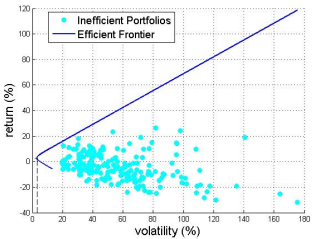
\includegraphics[scale=0.65]{img/Efficient_Frontier.png}
      \end{center}
    \end{example}

    \begin{example}[All Long Positions]
      Note that this efficient portfolio allows us to have unlimited short positions, which may or may not be realistic. If we wanted to work only with all-long portfolios, then we would impose the nonlinear restrictions 
      \begin{equation}
        0 \leq w_k \leq 1 \text{ for } k = 1, \ldots, K
      \end{equation}
      which would need to be solved numerically, possibly using nonlinear models. 
    \end{example}

    \begin{example}[Efficient Frontier with Risk-Free Asset]
      If we include a risk-free asset such as cash $C$ with risk-free return $R_f$ to the portfolio $\{P_1, \ldots, P_K\}$, then we slightly modify our equations. By definition, the risk-free asset has volatility $\sigma_0 = 0$ and its weight must be equal to $w_f = 1 - \sum_{i=1}^K w_k$
      , so we still want to minimize the same objective subject to constraint equations 
      \begin{equation}
        R_f \bigg( 1 - \sum_{k=1}^K w_k \bigg) + \sum_{k=0}^K w_k R_k = R
      \end{equation}

      When we allow our portfolio to include the risk-free security, the efficient frontier becomes a straight line that is tangential to the risky efficient frontier and with a $y$-intercept equal to the risk-free rate. 
      \begin{center}
        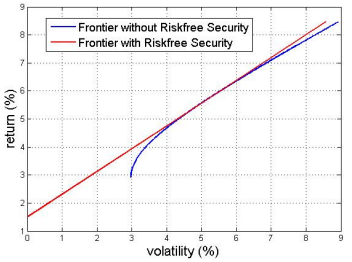
\includegraphics[scale=0.65]{img/Frontier_with_Risk_Free_Sec.png}
      \end{center}
      We can include other linear portfolio constraints, such as no-borrowing, no-short sales, or certain sector constraints. While analytic solutions are generally no longer available, the resulting problems are easy to solve numerically. 
    \end{example}

  \subsection{Capital Asset Pricing Model}

    Let us have some stock $P$ with random variable of return $R_p = R_{P, [i, j]}$ and the market $M$ with random variable of return $R_m = R_{M, [i, j]}$, both within period $[i, j]$. There may be some sort of risk-free return $r_f$ available (e.g. U.S. treasury bonds), so we can observe the returns of these two assets past the risk-free return by considering the joint distribution 

    \begin{equation}
      (R_p - r_f) \times (R_m - r_f)
    \end{equation}

    This may or may not be correlated, but the capital asset pricing model shows that there exists a linear relationship between the expected values of these two distributions. The central insight of the CAPM is that in equilibrium the riskiness of an asset is not measured by the standard deviation of its return but by its beta. 

    \begin{theorem}[CAPM]
      Now let $\overline{R}_m = \mathbb{E}[R_m]$ denote the expected return of the market, and $\overline{R} = \mathbb{E}[R]$ denote the expected return of a security or portfolio. Then, the \textbf{capital asset pricing model (CAPM)} asserts that there exists a linear relationship 
      \begin{equation}
        \overline{R} = r_f + \beta (\overline{R}_m - r_f)
      \end{equation}
      where $r_f$ is the risk-free rate. 
    \end{theorem}
    \begin{proof}
      Let us consider a portfolio of weights $\alpha$ and $1 - \alpha$ on the risky security and market portfolio, respectively. Let $R_\alpha$ denote the random return of this portfolio as a function of $\alpha$. We then have 
      \begin{align*}
          \mathbb{E}[R_\alpha] & = \alpha \overline{R} + (1 - \alpha) \overline{R}_m \\
          \mathrm{Var}(R_\alpha) & = \alpha^2 \mathrm{Var}(R) + (1 - \alpha)^2 \mathrm{Var}(R_m) + 2 \alpha (1 - \alpha) \mathrm{Cov}(R, R_m)
      \end{align*}
      Note that as $\alpha$ varies, the mean and standard deviation $(\mathbb{E}[R_\alpha], \mathrm{Var}(R_\alpha))$ trace out a curve in $\mathbb{R}^2$ that cannot cross the efficient frontier, as shown in the dotted line. 
      \begin{center}
          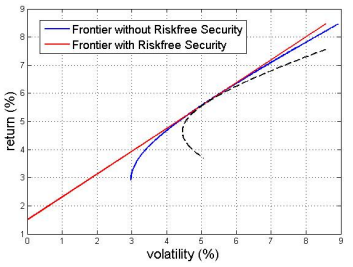
\includegraphics[scale=0.5]{img/CAPM.png}
      \end{center}
      At $\alpha = 0$, the slope of this curve must equal the slope of the capital market line. The slope of the $\alpha$-curve (where $\sigma(R_\alpha) = \sqrt{\Var(R_\alpha)}$) is 
      \begin{align*}
          \frac{d \mathbb{E}[R_{\alpha}]}{d \sigma(R_\alpha)} \bigg|_{\alpha = 0} & = \frac{d\mathbb{E}[R_\alpha]}{d \alpha} \bigg/ \frac{d \sigma(R_\alpha)}{d \alpha} \bigg|_{\alpha = 0} \\
          & = \frac{\sigma(R_\alpha) (\overline{R} - \overline{R}_m)}{\alpha \sigma(R) - (1 - \alpha) \Var (R_m) + (1 - 2 \alpha) \mathrm{Cov}(R, R_m)} \bigg|_{\alpha = 0} \\
          & = \frac{\sigma(R_m) (\overline{R} - \overline{R}_m)}{-\Var(R_m) + \mathrm{Cov}(R, R_m)}
      \end{align*}
      The slope of the capital market line is $(\overline{R}_m - r_f) / \sigma(R_m)$, and equating the two 
      \begin{equation}
        \frac{\sigma(R_m) (\overline{R} - \overline{R}_m)}{-\Var(R_m) + \mathrm{Cov}(R, R_m)} = \frac{\overline{R}_m - r_f}{\sigma(R_m)}
      \end{equation}
      gives the result. 
    \end{proof}

  \subsection{Efficient Market Hypothesis and No-Arbitrage Principle}

    \begin{definition}[Arbitrage Portfolio]
      Let us have some portfolio, which a value that is a stochastic process $V (t)$. It is considered an \textbf{arbitrage portfolio} if its current value $V(t) \leq 0$ and there exists some $T > t$ s.t. 
      \begin{equation}
        \mathbb{P}[V(T) \geq 0] = 1 \text{ and } \mathbb{P}[V(T) > 0] > 0
      \end{equation}
    \end{definition}

    \begin{theorem}[Axiom of No Arbitrage]
      There exists no arbitrage portfolios, i.e. there is no free lunch. 
    \end{theorem}

    This is indeed what one would consider an arbitrage portfolio in the colloquial sense. If you had positive capital to invest, $V(t) > 0$, then you can invest it in risk-free Treasury bonds, and you have a guarantee increase in value. This is why you need to start with no or negative capital. If you have $0$ cash, you can borrow at a risk free rate $r$, but if you use that to invest in treasury bonds, you are also getting returns at rate $r$, cancelling out the effects. 

    The first probability $\mathbb{P}[V(T) \geq 0] = 1$ is needed since it must be a guaranteed profit. If you have some cash on you, whether it'd be through a loan or you start off with some, you could take a coin flip bet to double your cash or lose all of it. If you win and indeed double it, this does not say anything about the theorem since the probability of this increase was not $1$. 

    \begin{theorem}[Monotonicity Theorem]
      Assume no arbitrage. If we have portfolios A and B s.t. for some point in time $T$ 
      \begin{equation}
        \mathbb{P}[V^A (T) \geq V^B (T)] = 1 
      \end{equation}
      then $V^A (t) \geq V^B (t)$ for all $t$. In addition, if $\mathbb{P}[V^A (T) > V^B (T)] > 0$, then the inequality is strict, i.e. $V^A (t) > V^B (t)$. 
    \end{theorem}
    
    \begin{corollary}[Equality]
      If $\mathbb{P}[V^A (T) = V^B (T)] = 1$, then $V^A (t) = V^B (t)$ for all $t$. 
    \end{corollary}

  \subsection{Replication Principle and Monotonicity Theorem}

    \begin{theorem}[Replication Principle]
      If we have two portfolios that have equal value at one point in time. Then they should have equal value at every other point in time. 
    \end{theorem}

    This leads to another 

\section{Derivatives}

  \begin{definition}[Derivatives]
    A \textbf{derivative} is a financial instrument whose value depends on (is \textit{derived} from) the value of some other, more basic, underlying variable. Essentially, given some stochastic process $X_t$ describing some variable, the derivative is some function 
    \begin{equation}
      Y_t = g(X_t)
    \end{equation}
    The reason that we say an underlying \textit{variable} is that it includes real assets (e.g. property), financial assets (e.g. stocks), indices (stock, inflation, or housing price index), or an event (e.g. weather, or the amount of rainfall in a given season to hedge against a bad winter). Therefore, these variables can be anything, like the number of people attending a fair, which may be an indicator of the profit of the fair or some catastrophic event, and we can derive value out of that event. Therefore, the variable does not necessarily have to be an asset. 
  \end{definition}

    The most common underlying assets for derivatives are: 
    \begin{enumerate}
      \item stocks
      \item bonds
      \item other derivatives 
      \item commodities
      \item currencies
      \item interest rates 
      \item market indexes 
    \end{enumerate}
    They can be traded either OTC (between 2 companies privately) or on an exchange.\footnote{OTC derivatives constitute a greater proportion of the derivatives market, but exchange-traded derivatives have many advantages, such as standardization, liquidity, and elimination of default risk. Originally, derivatives were used to ensure balanced exchange rates for goods traded internationally. With the differing values of national currencies, international traders needed a system to account for differences. }

    \begin{example}[Apples and Pies] 
      Suppose you have an apple orchard and you make pies. You can sell apples and pies at a fixed price, but you can also sell them at a future price. For example, you can sell apples at a future price of \$1 per apple. 
    \end{example}

    \begin{example}[Weather Derivatives]
      A weather derivative can have payout of $g(S_T)$, where 
      \begin{equation}
        g(S_T) = \mathbbm{1} \{S_T > 50\} = \begin{cases} \$1 & \text{ if } S_T > 50 \\ 0 & \text{ if else} \end{cases}
      \end{equation}
      where $S_T$ is the total snowfall in inches during the year up to $T = 1$. Note that both $S_T$ and $g(S_T)$ are random variables whose value is unknown until $T = 1$.
    \end{example}

    The three fundamental derivative contracts we will work with are forwards/futures, swaps, and options. Let's provide a brief summary of them. Forwards are the simplest type of contract and are the easiest to value. Additionally, through them we can define the forward price of any financial asset, which is essential for more complex valuation models. Futures are exchange-traded, futures-settled versions of forwards. Swaps are contracts where two parties agree to exchange cash flows based on some underlying asset. Options are contracts that give the holder the right, but not the obligation, to buy or sell an asset at a fixed price and are the most complex. They have many interesting properties. 

\section{Forward Contracts and Forward Prices} 

    Now we will see the most common type of derivative: the forward contract. 

    \begin{definition}[Forward Contracts]
      \textbf{Forward contracts} are contracts between two parties to buy or sell an asset at a future date for a price agreed upon today. For notation, let's write
      \begin{enumerate}
        \item $T$ is the time until delivery, usually in years. This is fixed per contract.
        \item $K$ is the delivery price. This is also fixed per contract. 
        \item $S_t$ is the spot price of the asset at time $t \in [0, T]$.
        \item $V_{K} (t, T)$ be the \textbf{true value} of the contract at current time $t \leq T$ of being long a forward contract with delivery price $K$ and maturity $T$. 
        \item The \textbf{price} is a noisy estimate of $V$. Let $P_t$ be the price of a long forward. 
      \end{enumerate}
    \end{definition}

    Note that $V_K (t, T)$ is what everyone wants to find out but is extremely difficult. However, there are some properties that it must satisfy. 

    \begin{lemma}[Value at Maturity, Payout]
      Since the party that longs the forward contract must pay $K$ at $T$ to buy an asset which is worth $S_T$, the value of the contract at $T$ is 
      \begin{equation}
        V_K (T, T) = S_T - K
      \end{equation}
      This is referred to as the \textbf{value at maturity} or the \textbf{payout} of the contract.
    \end{lemma}

    \begin{example}[Red Sox]
      If I buy the Boston Red Sox regular season wins at 100, in size one dollar per won, I have a long forward position with delivery price of 100. If the Red Sox wins 110 games I make \$10, and if they have 91 wins I lose \$9. The payout is $S_T - K$ where $S_T$ is the number of wins. 
      \begin{figure}[H]
        \centering 
        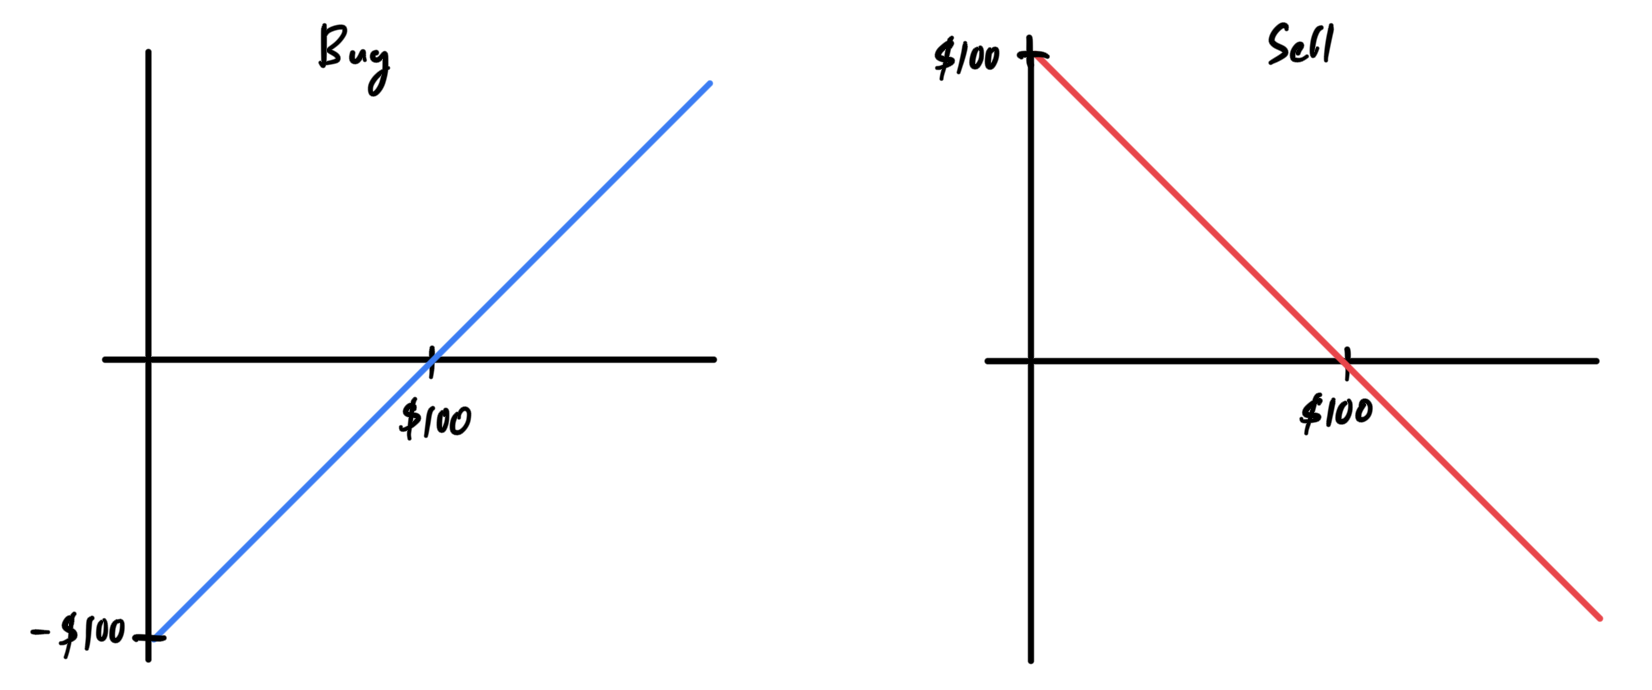
\includegraphics[scale=0.4]{img/forward_example.png}
        \caption{Payoff (not profit-loss) graphs for the buyer and sellers of the Red Sox contract. } 
        \label{fig:foward_example}
      \end{figure}
    \end{example}

  \subsection{Contract Specifications}
  
    Forward contracts are in general traded OTC, with two parties agreeing to the terms of the contract. This also means that there isn't a clearinghouse to guarantee the contract, so there is a risk of default. Post-2008, there has been a push to move towards exchange-traded contracts, which are standardized and have a clearinghouse to guarantee the contract. Regulations are done by the CFTC (Dodd-Frank Act expands CFTC oversight to OTC markets due to 2008). Accounting (does unrealized gains count as taxable income?) and taxes can be country specific. 

    \subsubsection{Settlement}

      Second, forwards go through \textbf{stock-type settlement} meaning that no cash flows happen until the delivery date. These can be physically settled or cash settled also. 

      \begin{definition}[Physical Settlement]
        If a contract is \textbf{physically settled}, it means that the buyer actually pays $K$ and receives the asset at time $T$. 
      \end{definition}

      \begin{definition}[Cash Settlement]
        However, some forwards are \textbf{cash settled}, meaning one simply receives (pays if negative) the amount $S_T - K$ at time $T$.\footnote{For example, if you look at forwards on the SP500 index, you must cash settle since you can't deliver fractional shares. }
      \end{definition}

      The profit/loss is the same, but there are some key differences. A cash settled forward has no further exposure to the asset price since you're just receiving the difference in cash. However, a physically settled contract implies that the buyer now owns the asset at $T$, which continues to have exposure to asset price movements. 

      \begin{definition}[Stock-Type Settlement]
        \textbf{Stock-type settlement} means that no cash flows happen until the delivery date.
      \end{definition}

      \begin{exercise}[Hull 1.5]
        An investor enters into a short forward contract to sell $100,000$ British Pounds for US dollars at an excahnge rate of $1.5$ dollars per pound. How much does the investor gain or lose if the exchange rate at the expiration date is $1.4900$ dollars per pound? What if it is $1.5200$ dollars per pound?\footnote{A \textbf{pip} is 1/100 of a cent.}
      \end{exercise}
      \begin{solution}
        Note that we must specify the currency of the profit or loss. It turns out that the payoff will always be in the currency that the investor is selling. The investor is selling the forward, so they are obligated to sell it at $1.5000$ dollars per pound. 
        \begin{enumerate}
          \item If the rate is $1.4900$, then the investor sells the pounds for $150,000$ USD and can buy a little bit more than $100,000$ pounds. In fact, they are making a profit of $100,000 \cdot 0.0100 = 1,000$ dollars.
          \item If the rate is $1.52$, then the investors sells the pounds for $150,000$ USD and can buy a little less than $100,000$ pounds, so they lose $100,000 \cdot 0.0200 = 2,000$ dollars. 
        \end{enumerate}
      \end{solution}

  \subsection{Forward Price}

    When A and B enter into a forward contract, it should be the case that the value of this contract should be $0$ when both parties agree to it. To see why, consider the following equivalent scenarios between parties A and B, with interest rates being 10\%.\footnote{Thanks to \href{https://www.quora.com/Why-is-the-initial-value-of-a-forward-contract-set-to-zero}{this Quora post} for clarifying. } 

    \begin{enumerate}
      \item \textbf{A} must buy some product at \$400 from \textbf{B} in 1 year, which has a value of $0$ for both parties.  
      \item \textbf{A} must buy some product at \$300 from \textbf{B} in 1 year \textit{and} \textbf{A} must give \textbf{B} \$90.91 now (present value of \$100 in 1 year). The forward itself has positive value for \textbf{A} and negative value for \textbf{B}. 
      \item \textbf{A} must buy some product at \$500 from \textbf{B} in 1 year \textit{and} \textbf{B} must give \textbf{A} \$90.91 now. The forward itself has positive value for \textbf{B} and negative value for \textbf{A}. 
    \end{enumerate}
    Note that the second and third points are the same as initiating a $0$-value forward contract plus a separate loan. In scenario 2, \textbf{A} is loaning \textbf{B} \$90.91, which means that \textbf{A} is expected to receive \$100 and pay \$400 for the product, which is equivalent to paying \$300 for the product. This goes for scenario 3, where \textbf{B} now loans \textbf{A} \$90.01. 

    While this fact was obvious from the start, this scenario really emphasizes that the delivery price, along with the time period and interest rates, is a huge determinant in the value of the forward. A lower delivery price means positive value to the buyer (and negative to seller), and a higher delivery indicates positive value to the seller (and negative to buyer). \footnote{Depending on the buyer and seller's estimates of the interest rates, these may differ, but for now we assume one true rate. }The specific price where this value is $0$ is called the \textit{forward price}.

    \begin{definition}[Forward Price]
      The \textbf{forward price} $F(t, T)$ at the current time $t \leq T$ is the delivery price $K$ such that 
      \begin{equation}
        V_K (t, T) = 0 \implies V_{F(t, T)} (t, T) = 0 
      \end{equation}
      That is, it is the price that makes the contract have zero value at the current time. 
    \end{definition}

    So we can think of the forward price as the fair price of an asset in the future, which is determined by the current spot price and the interest rate. 

    \begin{lemma}[Forward Price at Expiry]
      By definition, it must be the case that $F(T, T) = S_T$ since to buy an asset at $T$ for the price $F(T, T)$ is the same as buying the asset at the spot price $S_T$. 
    \end{lemma}

    When the forward is created, it has no intrinsic value, but as time goes on, the value of the contract changes as the spot price changes. So if you find that the strike is greater than the forward price, then the person who longs that contract would have to buy at a high price, meaning that the value is negative. Otherwise it is positive. 

    \begin{example}[Constant Stock]
      Suppose that a stock which pays no dividends always has price $100$ and interest rates are always $0$. Then 
      \begin{enumerate}
        \item $F(t, T) = 100$ since if you had the right to buy the stock at $100$ at any time $T$, then this would be the same as buying the stock at the spot market, but it is always $100$ in the spot market. So the value of this contract must be $0$ for all $T$. 
        \item $V_K (t, T) = 100 - K$ since if you have the right to buy the stock at $K$ in time $T$, the spot price will always be worth $100$ so you're really gaining $100 - K$. Therefore the value of this contract must be $100 - K$ for all $T$. 
      \end{enumerate}
    \end{example}

    To try valuing forward contracts through some formula, we should have an analogous formula for forward prices. Essentially, the fair value of our forward price should be captured in this formula.  
    \begin{align*}
      \text{forward price } = \text{current spot price of underlying} & + \text{benefits of buying later} \\ 
                                                                       & - \text{costs of buying later}
    \end{align*}
    Let's think about the benefits of buying later, which is equivalent to the costs of buying now. 
    \begin{enumerate}
      \item \textit{Interest on Cash.} You can get interest on the cash you have now.  
      \item \textit{Inventory Costs.} There are inventory costs that you would incur from storing products, e.g. commodities. There are also transportation and insurance costs.  
    \end{enumerate}
    The benefits of buying now, or the costs of buying later, is as such: 
    \begin{enumerate}
      \item \textit{Convenience Yield.} The buyer may urgently need the product now to capitalize on some immediate business opportunity. 
      \item \textit{Fixed Income Payments.} By not owning a dividend-paying stock or bond now, you will miss out on fixed-income payments like dividends or coupon payments. 
    \end{enumerate}
    The forward price is only dependent on the current underlying price $S_t$, the interest rate $r$, and the time to maturity $T - t$. Counterintuitively, it does not depend on the growth rate, the standard deviation, or any distributional assumptions of $S_T$. Furthermore, any two assets which pay no income and which have the same spot price $S_t$ will have the same forward price regardless of any views about their future movements. 
  
    Now we want to put this formula in more mathematical terms. Let's do this for underlying assets that gradually increase in complexity. 

    \begin{theorem}[Forward Price of No Income Asset]
      For an asset paying no income (e.g. a stock with no dividends), the forward price is 
      \begin{equation}
        F(t, T) = S_t \cdot Z_r (t, T)^{-1}
      \end{equation} 
    \end{theorem}
    \begin{proof}
      \textbf{Replication}. At current time $t$, let's take two portfolios. 
      \begin{enumerate}
        \item A: Consists of one unit of the underlying stock. 
        \item B: One long forward contract with delivery price $K$, plus $K e^{-r(T - t)}$ of cash. 
      \end{enumerate}
      At time $T$, B can invest the cash at the risk free rate $r$ and get $K$ cash. Then, it executes the forward contract at $K$ to get one stock. Therefore, at time $T$, both portfolios are worth $S_T$ and the values of both portfolios at time $t$ must also be the same. This is called the \textit{replication proof}. 
      \begin{equation}
        S_t = V_K (t, T) + K e^{-r (T - t)} \implies V_K (t, T)= S_t - K e^{-r (T - t)}
      \end{equation}
      We want to find the value of $K$ such that the value of the contract is $0$. Therefore, 
      \begin{equation}
        0 = S_t - K e^{-r (T - t)} \implies K = S_t e^{r (T - t)}
      \end{equation}
    \end{proof}
    \begin{proof}
      \textbf{No Arbitrage}. Another way to prove this is with the \textbf{No-arbitrage principle}. What we do is assume that the forward value is above or below our stated value, and prove that under these assumptions there is an arbitrage opportunity. 
      \begin{enumerate}
        \item Assume that $F(t, T) < S_t e^{r (T - t)}$. Then, you can buy a forward contract at delivery price $K = F(t, T)$ for free. You can also short the underlying stock at $S_t$ and invest the proceeds at the interest rate $r$. At time $T$, you can take your money, which is now worth $S_t e^{r (T - t)}$ and execute the contract by buying one share of the stock for $K = F(t, T)$. This leaves you with no stocks and money of $S_t e^{r (T - t)} - F(t, T) > 0$ by assumption, and you have an arbitrage opportunity.
        \item Assume that $F(t, T) > S_t e^{r (T - t)}$. Then, you can sell a forward contract at delivery price $K = F(t, T)$ for free. I borrow $S_t$ money at the interest rate $r$ and buy a stock. At time $T$, I sell the stock at $F(t, T)$ and also must pay back from who I borrowed at a rate of $S_t e^{r (T - t)}$. Therefore, this leaves me with a net gain of $F(t, T) - S_t e^{r (T - t)} > 0$ by assumption, and I have an arbitrage opportunity.
      \end{enumerate}
      Therefore, since I have an arbitrage opportunity, it must be the case that $F(t, T) = S_t e^{r (T - t)}$.
    \end{proof}

    Intuitively, with the no arbitrage strategy, we can see that if the forward price is too high relative to the stock price $S_t$, we buy the stock now and sell the contract (sell the stock forward at the higher price). If the forward price is too low, then we sell the stock now and buy the contract (buy the stock forward at the cheaper price).

    \begin{exercise}[Blyth Chapter 2 Exercise 2]
      At time $t$ you own one stock that pays no dividends, and observe that 
      \begin{equation}
        F(t, T) < \frac{S_t}{Z(t, T)} 
      \end{equation}
      What arbitrage opportunity is available to you, assuming you can only trade the stock, ZCB, and the forward contract? 
    \end{exercise}

    \begin{solution}[Blyth Chapter 2 Exercise 2]
      Note that if we rearrange the equation, it becomes 
      \begin{equation}
        F(t, T) \; Z (t, T) < S_t
      \end{equation}
      This should really be an equality, so it tells us that at least the LHS is undervalued, or the RHS is overvalued. So we want to take long positions on the forward price and the ZCB, while we take a short position on $S_t$. 
      \begin{enumerate}
        \item We can first short-sell the stock at $S_t$ and buy a forward contract for no cost.\footnote{If you're betting that the forward price will go up, then this means that it is advantageous to buy the contract so you can lock in a lower forward price to buy the underlying later. }
        \item We now have $S_t$ in cash, which we loan it out at the ZCB rate.\footnote{If we are betting that the ZCB value, i.e. the present value of \$1, will go up, then this means that interest rates will decrease. If interest rates decrease, you would like to loan \textit{now} rather than later to make a profit. }

        \item At time $T$, you have $S_t / Z(t, T)$ in cash. You use this to buy back the stock at the delivery price $F(t, T)$ (not the spot price $S_T$) from your forward contract, and you return this stock back to the lender who you shorted-sold. Therefore, you are left with 
          \begin{equation}
            \frac{S_t}{Z(t, T)} - F(t, T) > 0 
          \end{equation}
          in cash. 
      \end{enumerate}
    \end{solution}
    
    \begin{exercise}[Blyth Chapter 2 Exercise 1]
      Let $S_t$ be the current price of a stock that pays no dividends. 
      \begin{enumerate}
        \item Let $r_{\mathrm{bid}}$ be the interest rate at which one can invest/lend money, and let $r_{\mathrm{off}}$ be the interest rate at which one can borrow money, $r_{\mathrm{bid}} \leq r_{\mathrm{off}}$. Both rates are continuously compounded. Using arbitrage arguments, find the upper and lower bounds for the forward price of the stock for a forward contract with maturity $T > t$. 

        \item How does your answer change if the stock itself has bid price $S_{t, \mathrm{bid}}$ and offer price $S_{t, \mathrm{off}}$? 
      \end{enumerate}
    \end{exercise}

    \begin{solution}[Blyth Chapter 2 Exercise 1]
      Let's go through two cases. Assume you start with nothing. 
      \begin{enumerate}
        \item You can short-sell a stock at $S_t$, loan out the $S_t$ in cash at rate $r_{\mathrm{off}}$, and buy a forward contract at some forward price $F(t, T)$. At time $T$, you receive $S_t e^{r_{\mathrm{off}} (T - t)}$ and can buy the stock at some forward price to return. In this case, we would have arbitrage if the money I am left with
        \begin{equation}
          S_t e^{r_{\mathrm{off}} (T - t)} - F(t, T) > 0
        \end{equation}
        so this can't be the case. 

        \item You can borrow $S_t$ in cash at the rate $r_{\mathrm{bid}}$, immediately buy a stock at $S_t$, and sell a forward at some forward price $F(t, T)$. At time $T$, I can sell the stock at price $F(t, T)$ and then use this money to pay back my loan. We would have arbitrage if the money I am left with 
        \begin{equation}
          F(t, T) - S_t e^{r_{\mathrm{bid}} (T - t)} > 0
        \end{equation}
      \end{enumerate}
      Neither of these can occur by the no arbitrage principle, so we have the bounds 
      \begin{equation}
          S_t e^{r_{\mathrm{bid}} (T - t)} < F(t, T) < S_t e^{r_{\mathrm{off}} (T - t)}
      \end{equation}
      If the stock had a bid-ask price, then we can slightly adjust our formula. In the first scenario, we short sell a stock at the bid price, and in the second, we buy a stock at the ask price. Therefore, we have 
      \begin{equation}
        S_{t, \mathrm{ask}} e^{r_{\mathrm{bid}} (T - t)} < F(t, T) < S_{t, \mathrm{bid}} e^{r_{\mathrm{off}} (T - t)}
      \end{equation}
    \end{solution}

    However, this is unrealistic in a few things. It first does not account for dividends, the cost of storage, or the cost of carry. 

    \begin{theorem}[Forward Price of Income Asset]
      Suppose an asset pays a known amount of income (e.g. dividends, coupons, rent) during the life of the forward contract and the present value at $t$ of the income is $I$. Then, 
      \begin{equation}
        F(t, T) = (S_t - I)e^{r(T - t)}
      \end{equation}
    \end{theorem}
    \begin{proof}
      \textbf{Replication}. Let us have two portfolios. 
      \begin{enumerate}
        \item A: Consists of one unit of the underlying stock. 
        \item B: Consists of one long forward contract with delivery price $K$, plus $K e^{-r(T - t)} + I$ of cash. 
      \end{enumerate}
      Then, B will invest the cash at the risk free rate $r$ and get $K + I e^{r(T - t)}$ cash. Then it uses $K$ to buy the underlying stock, ending up with $I e^{r(T - t)}$ in cash and one unit of stock. A, by owning the stock throughout the span, also receives $I$ of cash (present value), which is equal to $I e^{r(T - t)}$ worth at time $T$. Therefore, the two portfolios are equal at time $T$ and therefore must be equal at time $t$. 
      \begin{equation}
        S_T + I e^{r(T - t)} = V_K (T, T) + K + I e^{r(T - t)} \implies S_t = V_K (t, T) + K e^{-r(T - t)} + I
      \end{equation}
      Therefore, we can solve for the forward price by setting $V_K(t, T) = 0$. 
      \begin{equation}
        S_t = K e^{-r(T - t)} + I \implies F(t, T) = K = (S_t - I) e^{r(T - t)}
      \end{equation}
    \end{proof}
    \begin{proof}
      \textbf{No Arbitrage}. We assume the two scenarios. 
      \begin{enumerate}
        \item $F(t, T) < (S_t - I) e^{r(T - t)}$. Then, we buy the forward contract for free at $K = F(t, T)$ and short the stock at $S_t$. We take the proceeds of the short and invest it at the risk free rate $r$. At time $T$, we buy back the stock at $F(t, T)$, and give back the stock to the lender, and additional pay them the dividends they would have received, which is $I e^{r(T - t)}$. Therefore, our net profit is
          \begin{equation}
            S_t e^{r(T - t)} - F(t, T) - I e^{r(T - t)} > 0
          \end{equation}
        \item $F(t, T) > (S_t - I) e^{r(T - t)}$. Then, we buy the stock at $S_t$ and short the forward contract at $K = F(t, T)$ for free. At time $T$, we get our income $I e^{r(T - t)}$, pay back the lender at $S_t e^{r(T - t)}$, and execute the contract to sell it at $F(t, T)$. Our net profit is 
          \begin{equation}
            F(t, T) + I e^{r(T - t)} - S_t e^{r(T - t)} > 0
          \end{equation}
      \end{enumerate}
      Therefore, we have an arbitrage opportunity in both cases, and therefore it must be the case that $F(t, T) = (S_t - I) e^{r(T - t)}$.
    \end{proof}

    If the stock pays some income at a compounded rate, then we have the following result on the forward price. 

    \begin{theorem}[Forward Price of Compounded Income Asset]
      If the stock pays a continuous dividend yield $q$ (e.g. $q = 0.02$ means that the stock pays $2\%$ of its value in dividends each year), then the forward price is 
      \begin{equation}
        F(t, T) = S_t e^{(r - q)(T - t)}
      \end{equation}
    \end{theorem}

    \begin{theorem}[Forward Price of Forex]
      The forward price of one unit of foreign currency is given by 
      \begin{equation}
        F(t, T) = X_t e^{(r_{\$} - r_f) (T - t)}
      \end{equation}
      where $X_t$ is the price at time $t$ of one foreign currency and $T$ is the maturity of the forward contract. 
    \end{theorem}
    \begin{proof}
      We use replication. Consider the two portfolios. 
      \begin{enumerate}
        \item You start off with $X_t$ dollars, which you immediately convert to $1$ foreign currency and put it in interest to get $e^{r_f (T - t)}$ foreign currency at time $T$. 
        \item You start off with $X_t$ dollars. You immediately buy a forex forward at $F(t, T)$ for no cost and put the dollars in interest. At time $T$, we have $X_t e^{r_{\$} (T - t)}$ in cash. We execute the forward and convert our dollars to the foreign currency, leaving us with $\frac{X_t}{F(t, T)} e^{r_{\$} (T - t)}$ foreign currency. 
      \end{enumerate}
      By replication these two portfolios must equal in value, and we have 
      \begin{equation}
        \frac{X_t}{F(t, T)} e^{r_{\$} (T - t)} = e^{r_f (T - t)} \implies F(t, T) = X_t e^{(r_{\$} - r_f) (T - t)}
      \end{equation}
    \end{proof}

    At this point, we can take any financial security and interpret the forward price of it as the fair price of it at some predetermined point in the future. 

    \begin{example}[Forward Price of Commodities]
      The forward price of a commodity is 
      \begin{equation}
        F(t, T) = S_t (1 + r (T - t)) + s (T - t) + i (T - t)
      \end{equation}
      where $s, i$ are the annual storage, insurance costs per commodity unit.\footnote{This assumes no compound interest (?) } If these values are known, you can use them to predict other variables like the potential convenience yield. 
    \end{example}

    \begin{example}[Forward Price of Dividend-Paying Stock]
      Let 
      \begin{enumerate}
        \item $S_t$ be the stock price 
        \item $r$ be the interest rate over the life of the forward contract 
        \item $d_i$ is each dividend payment expected prior to maturity of the forward contract 
        \item $t_i$ is the time remaining to maturity after each dividend payment. 
        \item $r_i$ the applicable interest rate (i.e. \textit{forward rate}) from each dividend payment to maturity of the forward contract. 
      \end{enumerate}
      Then, the forward price of a dividend-paying stock can be written as the cash plus all the dividend payments, plus their interest. 
      \begin{equation}
        F(t, T) = S(1 + r (T - t)) - \sum_{i} d_i (1 + r_i t_i)
      \end{equation}
    \end{example}

    \begin{example}[Forward Price of Bond]
      Let 
      \begin{enumerate}
        \item $r$ be the interest rate over the life of the forward contract 
        \item $c_i$ be each coupon expected prior to the maturity of the forward contract 
        \item $t_i$ be the time remaining to maturity after each coupon payment 
        \item $r_i$ be the applicable interest rate from each coupon payment to maturity of the forward contract
      \end{enumerate}
      Then, the forward price of a bond can be written as 
      \begin{equation}
        F(t, T) = B(1 + r(T - t)) - \sum_i c_i (1 + r_i t_i)
      \end{equation}
    \end{example}

    \begin{exercise}[Blyth Chapter 2 Exercise 4]
      FX forwards are among the most liquid derivative contracts in the world and often reveal more about the health of money markets (markets for borrowing or lending cash) than published short-term interest rates themselves.
      \begin{enumerate}
        \item On 3 October 2008, the euro dollar FX rate was trading at €1=\$1.3772,and the forward price for a 3 April 2009 forward contract was \$1.3891. Assuming six-month euro interest rates were 5.415\%, what is the implied six-month dollar rate? Both interest rates are quoted with act/360 daycount and semi-annual compounding. There are 182 days between 3 October 2008 and 3 April 2009.
        \item Published six-month dollar rates were actually 4.13125\%. What arbitrage opportunity existed? What does a potential arbitrageur need to transact to exploit this opportunity?
        \item During the financial crisis, several European commercial banks badly needed to borrow dollar cash, but their only source of funds was euro cash from the European Central Bank (ECB). These banks would: borrow euro cash for six months from the ECB; sell euros/buy dollars in the spot FX market; and sell dollars/buy euros six months forward (to neutralize the FX risk on their euro liability). Explain briefly how these actions may have created the arbitrage opportunity in (2), which existed for several months in late 2008.
      \end{enumerate}
    \end{exercise}

    \begin{solution}[Blyth 2.4]
      We will ignore the daycount conventions. We can substitute these values in the forward prices for forex to get 
      \begin{equation}
        1.3891 = 1.3772 \cdot e^{(r_{\$} - r_f) \cdot 0.5} \implies r_{\$} = 0.07138
      \end{equation}
      Therefore, the general idea is that we want to long domestic interest rates and short foreign interest rates, which means that we want to buy domestic bonds and sell foreign bonds.  
    \end{solution}

  \subsection{Valuation}

    \begin{theorem}[Valuation of Forward Contracts]
      The value of a forward contract on an asset satisfies 
      \begin{equation}
        V_K (t, T) = \big( F(t, T) - K \big) Z_r (t, T)
      \end{equation}
      which is the difference between the forward price and the delivery price, discounted back to today. 
    \end{theorem}
    \begin{proof}
      \textbf{No Arbitrage}. We assume the two scenarios.
    \end{proof}

    Note that for fixed $t_0, T$ with varying $t_0 \leq t \leq T$,  
    \begin{equation}
      V_{F(t_0, T)} (t, T) = 0 \text{ for } t = t_0
    \end{equation}
    and may not be $0$ as $t$ changes. However, 
    \begin{equation}
      V_{F(t, T)} (t, T)
    \end{equation}
    is constantly $0$. 

  \subsection{Forward Rates}

    One might want to borrow money at a future time, say from $T_1$ to $T_2$, but they are not sure what the interest rate will be. Therefore, they can buy a forward contract that expires at $T_1$, with an underlying zero coupon bond that has maturity of $T_2$. This essentially allows them to lock in the interest rate $r_{T_1, T_2}$ for a future loan between $T_1$ and $T_2$. This is called the \textit{forward rate}. 

    \begin{definition}[Forward Rate]
      The \textbf{forward rate} at current time $t$ for period $T_1$ to $T_2$ ($t \leq T_1 \leq T_2$) is the interest rate $f_{12}$ (agreed at $t$) at which one can borrow or lend money from $T_1$ to $T_2$. 

      \begin{figure}[H]
        \centering 
        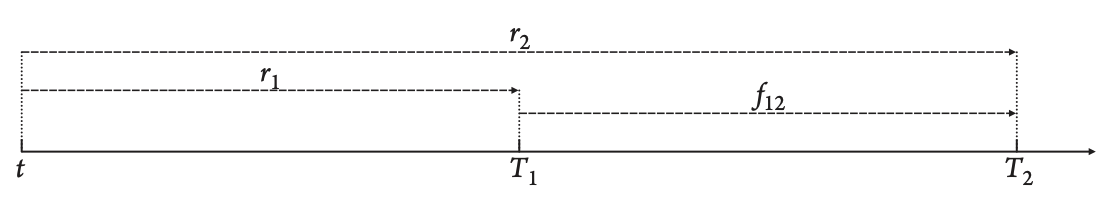
\includegraphics[scale=0.35]{img/forward_zero_rates.png}
        \caption{Common visual of forward rate, from Blyth.}
        \label{fig:forward_zero_rates}
      \end{figure}
    \end{definition}

    A simple replication argument gives the following result about the forward rate. 

    \begin{theorem}[Forward Rate]
      At time $t$, the fair value of the forward rate $f_{12}$ is given by 
      \begin{equation}
        Z_{r_1} (t, T_1) Z_{f_{12}} (T_1, T_2) = Z_{r_2} (t, T_2)
      \end{equation}
      where $r_k$ is the zero interest rate to borrow from $t$ to $T_k$. 
    \end{theorem}
    \begin{proof}
      This is trivial using the replication argument.
    \end{proof}

    This is great theoretically, but how do we actually trade something like this? What if we wanted to bet that this forward rate was going to be less than some percentage? We can do this by trading forward contracts with the underlying being ZCBs! As stated in the theorem below, the forward price of zero coupon bonds is precisely the same as the value of a zero coupon bond with the forward rate, which we can think of as locking in a future interest rate from $T_1$ to $T_2$.  

    \begin{theorem}[Forward Price equals Value of ZCB at Forward Rate]
      For $T_1 \leq T_2$, consider a forward contract with maturity $T_1$ on a ZCB with maturity $T_2$. That is, the underlying asset price is $S_t = Z(t, T_2)$. Then, the forward price, i.e. the price where one can (for no cost) agree to buy a forward contract on the $T_2$-ZCB with a expiry date of $T_1$, is 
      \begin{equation}
        F(t, T_1, T_2) = Z_{f_{12}} (T_1, T_2) = \frac{Z_{r_1} (t, T_2)}{Z_{r_2} (t, T_1)}
      \end{equation}
      Therefore, if we model the interest as simply compounded, we have 
      \begin{equation}
        F(t, T_1, T_2) = (1 + f_{12})^{-(T_2 - T_1)}
      \end{equation}
      and continuously compounded gives 
      \begin{equation}
        F(t, T_1, T_2) = e^{ -f_{12} (T_2 - T_1)}
      \end{equation}
    \end{theorem}
    \begin{proof}
      We can directly calculate the forward price of the underlying ZCB. It's a one-time payment of $1$ at time $T_2$, so the only cost to consider here is the time value of money. Therefore, $F(t, T_1, T_2) = Z_{f_{12}} (T_1, T_2)$, and the second equality follows from the forward rate identity above.\footnote{Note that this is not trivial as reducing them to exponentials! This was just proved in the previous theorem. } 
    \end{proof}

    \begin{example}[Forward Libor Rate]
      
    \end{example}

    \begin{exercise}[Blyth 3.1]
      Suppose $t \leq T_1 \leq T_2 \leq T_3$, where $t$ is current time, and $\varepsilon > 0$. Recall that $Z(T_1, T_2)$ is the price at time $T_1$ of a ZCB with maturity $T_2$, and $F(T_1, T_2, T_3)$ is the forward price at time $T_1$ for a forward contract with maturity $T_2$ on a ZCB with maturity $T_3$.
      \begin{enumerate}
        \item For each of the pairs of A and B in Table 3.1, choose the most appropriate relation-ship out of $\geq$, $\leq$, $=$ and ?, where ? means the answer is indeterminate. Give brief reasoning.
        \item What can you say about interest rates between T1 and T2 if 
          \begin{enumerate}
            \item $Z(t,T1) = Z(t,T2)$ ?
            \item $Z(t,T1) > 0$ and $Z(t,T2) = 0$?
          \end{enumerate}
      \end{enumerate}
    \end{exercise}

    \begin{solution}[Blyth 3.1]
      For (1), the answers are listed. 
      \begin{enumerate}
        \item $Z(t, T_1) \leq 1$. Assuming positive interest rates, you discount $1$ to present value.  
        \item $Z(T_1, T_1) = 1$. You receive the money now so it's the same as $1$. 
        \item $Z(t, T_2) \geq Z(t, T_3)$. You lock up your money for longer until $T_3$, so it should be worth less. 
        \item $Z(T_1, T_2) \geq Z(T_1, T_3)$. Same as above.  
        \item $Z(T_1, T_3) \leq Z(T_2, T_3)$. You lock up your money for longer at $T_1$, so it's worth less. 
        \item $Z(T_1, T_1 + \Delta) \, ? \, Z(T_2, T_2 + \Delta)$. Indeterminate since you don't know what prevailing interest rates are. 
        \item $F(t, T_1, T_2) \geq F(t, T_1, T_3)$. Reduce them to the ZCB values from $T_1$ to $T_2$ and $T_1$ to $T_3$. You are now comparing $Z(t, T_2)$ and $Z(t, T_3)$, which from above, $Z(t, T_3)$ is worth less. 
        \item $F(t, T_1, T_3) \leq F(t, T_2, T_3)$. Same as above, but now you are comparing $Z(t, T_1)^{-1}$ and $Z(t, T_2)^{-1}$. 
        \item $\lim_{T \rightarrow \infty} Z(t, T) = 0$. If you are lending money for an infinite time, it's as if you don't have any money. Interest rates $r$ I suppose would rise though (?). 
      \end{enumerate}
      For (2), 
      \begin{enumerate}
        \item Either $T_1 = T_2$ or $f_{12} = 0$. 
        \item $f_{12} < 0$. 
      \end{enumerate}
    \end{solution}

    \begin{exercise}[Blyth 3.2]
      Forward Rates. 
      \begin{enumerate}
        \item The one-year and two-year zero rates are 1\% and 2\% respectively. What is the one-year forward rate (that is, $f_{11}$)? Assume all rates are annually compounded. 
        \item If the two-year forward one-year rate ($f_{21}$) is 3\%, what is the three-year zero rate? 
      \end{enumerate}
    \end{exercise}

\section{Swaps}

  \begin{definition}[Swap]
    \textbf{Swaps} are contracts through which two parties exchange cash flows or liabilities from two different financial instruments. One cash flow is generally fixed, while the other is variable and is based on a benchmark interest rate, floating currency exchange rate, or index price. 
    \begin{enumerate}
      \item $T_0$ is the start date, $T_n$ the maturity date, and $T_i$ the payment dates for $i = 1, 2, \ldots, n$. In vanilla swaps we will have $T_i + \alpha = T_{i+1}$ for fixed $\alpha$. 
      \item The \textbf{fixed leg} of the swap consists of payments $\alpha K$ at each payment date for some fixed \textbf{delivery price/rate} $K$. 
      \item The \textbf{floating leg} of the swap consists of payments $\alpha P_i$ for each payment date, where $P_i$ may be dependent on the variable benchmarks. 
    \end{enumerate}
  \end{definition}

  \subsection{Contract Specification} 

    The most common examples of swaps can be about: 
    \begin{enumerate}
      \item interest rates
      \item mortgage bonds 
      \item exchange rates
    \end{enumerate}
    Swaps don't trade on exchanges, and retail investors do not generally engage in swaps. Rather, swaps are over the counter contracts primarily between businesses that are customized to the needs of both parties. 

    \begin{definition}[Interest Rate Swaps]
      In \textbf{interest rate swaps}, we have 
      \begin{equation}
        P_i = L_{T_{i-1}} [T_{i-1}, T_{i}]
      \end{equation}
      where the variable payments are dependent on the Libor rate fixing at $T_{i-1}$ for the period $T_{i-1}$ to $T_{i} = T_{i-1} + \alpha$, paid at $T_i$. 
      \begin{figure}[H]
        \centering 
        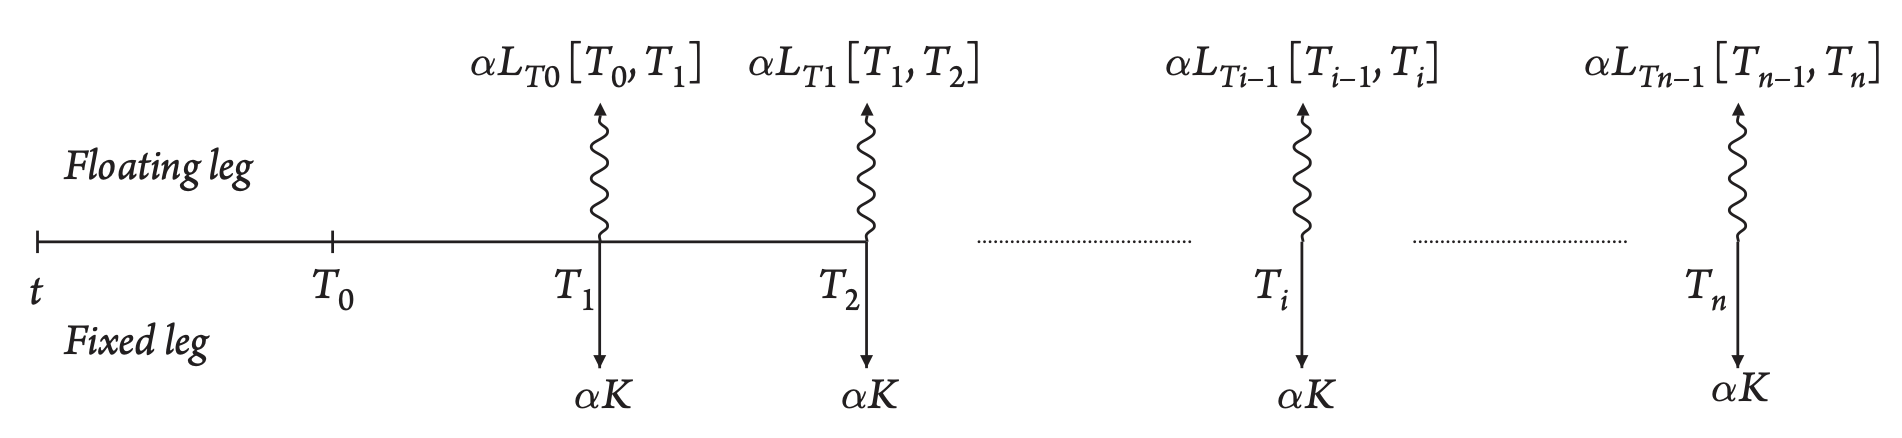
\includegraphics[scale=0.4]{img/interest_rate_swap.png}
        \caption{Visual of an interest rate swap. } 
        \label{fig:interest_rate_swap}
      \end{figure}
    \end{definition}

    \begin{definition}[Forex Swaps]
      
    \end{definition}

  \subsection{Forward Swap Rate and Swap Value}

  \subsection{Swaps as a Difference Between Bonds}

\section{Future Contracts}

  \begin{definition}[Futures]
    Like forward contracts, \textbf{future contracts} are contracts between two parties to buy or sell and asset at a future ate for a price agreed upon today. For notation, let's write 
    \begin{enumerate}
      \item $T$ is the time until delivery, usually in years. This is fixed per contract. 
      \item $K$ is the delivery price. This is also fixed per contract. 
      \item $S_t$ is the spot price of the asset at time $t \in [0, T]$. 
      \item $V_K (t, T)$ be the \textbf{true value} of the contract at current time $t \leq T$ of being long a future contract with delivery price $K$ and maturity $T$. 
      \item The \textbf{price} is a noisy estimate of $V$. Let $P_t$ be the price of a long future.
    \end{enumerate}
  \end{definition}
  
  The difference between futures and forwards is that first, futures are exchange traded and thus have standards to follow, and second, futures are settled daily. Future contracts are forwards contracts, but these extra factors slightly change the properties of the contract. 

  \subsection{Contract Specifications}

      We want to talk about 
      \begin{enumerate}
        \item What the \textbf{underlying} asset is. 

        \item The \textbf{contract size}. The price of the contract shown is usually for one unit of the underlying commodity, so the actual value of the contract is the price times the contract size. These sizes are determined by the exchange (should be large enough for institutions to be interested in but not too big to be unaffordable). Furthermore, the mini contracts are less liquid and have a higher big ask spread. 

        \item The \textbf{(expected) grade}, or quality, of the underlying, if applicable (e.g. commodities). This allows for a range of grades depending on the actual grade of the contract.  

        \item Delivery date and location, which may be slightly different than when the contract expires. 

        \item The minimum and maximum price change allowed in a day, and any price change beyond this limit will halt trading (called \textit{limit up} or \textit{limit down}). However, trading can still resume if it goes down. 

        \item The maximum number of contracts that a trader can hold. This is to prevent parties from cornering a market. 
      \end{enumerate}

    \subsubsection{Bond Futures}
      Let's start off with bonds. U.S. Treasury futures and options contracts are available for each of the U.S. Treasury benchmark tenors: 2-year, 5-year, 10-year, and 30-year. Additionally, CME Group offers Ultra 10-Year Note and Ultra T-Bond futures which offer greater precision for trading the 10-year and 30-year maturity points on the yield curve, respectively. Filling out the curve further, 3-Year Note futures (reintroduced in 2020) bring finer hedging granularity to the front of the curve, while 20-Year Bond futures (launched in 2022) provide a precise instrument for hedging 20-Year bond exposure. 

      Each of the bond and note futures contracts has an associated delivery bond basket that defines the range of bonds by maturity that can be delivered by the seller to the buyer in the delivery month. For example, the 5-year contract delivers into any U.S. government fixed coupon bond that has a remaining maturity of longer than 4 years and 2 months and an original maturity of no more than 5 years and 3 months. The delivery mechanism ensures the integrity of futures prices by ensuring that they are very closely tied to the prices of U.S. government bonds and their yields (interest rates). 

      When calculating the minimum tick size, they tend to say something like ``In percent of par to one-eighth of 1/32nd of 1\% of par,'' which means $0.01 \cdot 1/8 \cdot 1/32$ of the total contract size. Furthermore, the quotes are represented as a percentage of the face value, e.g. 103.23 would mean 103,230 for a \$100,000 contract. 

      \begin{table}[H]
        \centering
        \begin{tabular}{|l|l|l|l|}
        \hline
        \textbf{Underlying} & \textbf{Size} & \textbf{Increments} & \textbf{Deliverable Maturities} \\ \hline
        2-Year T-Note & \$200,000 & $\frac{1}{8} \cdot \frac{1}{32}$ c (\$7.8125) & 1 3/4 to 2 years \\ \hline
        3-Year T-Note & \$200,000 & $\frac{1}{8} \cdot \frac{1}{32}$ c (\$7.8125) & 2 9/12 to 3 years \\ \hline
        5-Year T-Note & \$100,000 & $\frac{1}{4} \cdot \frac{1}{32}$ c (\$7.8125) & 4 1/6 to 5 1/4 years \\ \hline
        10-Year T-Note & \$100,000 & $\frac{1}{2} \cdot \frac{1}{32}$ c (\$15.625) & 6 1/2 to 8 years \\ \hline
        Ultra 10-Year T-Note & \$100,000 & $\frac{1}{2} \cdot \frac{1}{32}$ c (\$15.625) & 9 5/12 to 10 Years \\ \hline
        T-Bond & \$100,000 & $\frac{1}{32}$ c (\$31.25) & 15 years up to 25 years \\ \hline
        20-Year T-Bond & \$100,000 & $\frac{1}{32}$ c (\$31.25) & 19 2/12 to 19 11/12 years \\ \hline
        Ultra T-Bond & \$100,000 & $\frac{1}{32}$ c (\$31.25) & 25 years to 30 years \\ \hline
        \end{tabular}
        \caption{Standards of Bonds Futures Contracts}
        \label{tab:bonds}
      \end{table}

      In practice, most participants trade U.S. Treasury futures contracts with the intent of either closing out the futures position or rolling them into longer expiry futures contracts. U.S. Treasury futures are listed on the March, June, September, and December quarterly cycles. More specifically, the futures expire in March, June, September, and December 24 of each year. This standard is consistent with the U.S. Treasury auctions, which take place in February, May, August, and November. 

      \begin{example}[Bond Futures Standards]
        Mathematically, this means that if the current time is $t$, the delivery date is $T_1$, and the bond maturity date is $T_2$, then for a futures on a 10-year T-Note, 
        \begin{enumerate}
          \item $T_1$ must be in one of the days of March, June, September, December 24. 
          \item $T_2 - T_1 \approx 10$. 
        \end{enumerate}
      \end{example}

      For bond futures, there is the concept of a \textbf{continuous contract}, which is a price of a certain type of contract that accounts for all the expiration dates. 

      \begin{question}
        Why do the prices of these futures increase as $T_1$ is further? 
      \end{question}

    \subsubsection{Equity Index Futures}

      Futures on stocks, called \textbf{single-stock futures}, are generally not very accessible for retail investors (e.g. OneChicago).\footnote{If you Google search ``Apple futures'' you don't really get anything. } Rather we use \textbf{stock index futures}, which we list some specs down in decreasing order of popularity. 

      \begin{table}[H]
        \centering
        \begin{tabular}{|l|l|l|l|l|}
        \hline
        \textbf{ADV}\footnote{Average Daily Volume} & \textbf{Underlying} & \textbf{Size} & \textbf{Increments} & \textbf{Ex. Quote} \\ \hline
        1,697,303   & E-Mini S\&P 500           & 50  & 0.25 (\$12.50)  & 5253.50 \\ \hline
        231,570     & E-Mini Nasdaq 100         & 20  & 0.25 (\$5.00)   & 18675.75\\ \hline
        160,145     & E-Mini Dow                & 5   & 1 (\$5.00)      & 38191 \\ \hline 
        19,487      & E-Mini S\&P MidCap 400    & 100 & 0.1 (\$10)      & 2918.60 \\ \hline
        12,599      & Nikkei 225 (USD)          & 5   & 5 (\$25)        & \\ \hline
        7839        & S\&P 500                  & 250 & 0.25 (\$62.50)  & 5412.75 \\ \hline
                    & E-Mini Russell 2000       & 50  & 0.10 (\$5.00)   & \\ \hline
                    & Micro E-Mini S\&P 500     & 5   & 0.25 (\$1.25)   & 5253.75 \\ \hline
                    & Micro E-Mini Nasdaq 100   & 2   & 0.25 (\$0.50)   & \\ \hline
                    & Micro E-Mini Dow          & 0.5 & 1 (\$0.50)      & \\ \hline
                    & Micro E-Mini Russell 2000 & 5   & 0.10 (\$0.50)   & \\ \hline
        \end{tabular}
        \caption{Standards of Equity Index Futures Contracts}
        \label{tab:equity_index}
      \end{table}

      These contracts, like bonds, trade during the months of March, June, September, and December. Trading terminates at 9:30 a.m. ET on the third Friday of the contract month.

    \subsubsection{Oil and Natural Gas Futures}

      The two main fuel commodities traded are crude oil and natural gas. Let's compare the two. 
      \begin{enumerate}
        \item Crude oil is used for vehicle fuel while natural gas is for stoves and electric lights. This difference in purpose and thus demand likely is the cause of the prices.  
        \item Crude oil needs to go under a heavy refining process while natural gas is minimal. 
        \item Crude oil is liquid at room temperature while natural gas is a gas. 
      \end{enumerate}

      \begin{definition}[Crude Oil]
        \textbf{Crude oil} is a naturally occurring, unrefined petroleum product composed of hydrocarbon deposits and other organic materials. It is primarily used to produce gasoline, diesel fuel, and other essential products, being liquid in room temperature. 

        Crude oil needs to undergo a refining process to convert into gasoline, and thus there are different grades of oil. 
        \begin{enumerate}
          \item \textbf{Light crude oil} is a type of crude oil that has a low density, measured by the American Petroleum Institute (API) gravity, and flows freely at room temperature.\footnote{API levels fall between 10 and 70, with higher numbers being lighter. Even light enough to float in water. } \textbf{Heavy crude oil} has higher density and is harder to refine. 
          \item \textbf{Sweet} oil refers to the sulfur content of the oil, with sweet oil having less than 0.5\% sulfur. \textbf{Sour} oil has more than 0.5\% sulfur. 
        \end{enumerate}
        The main premium oils that are traded are light sweet oils, with the two benchmarks being \textbf{West Texas Intermediate (WTI)}, which is extracted from fields located in Texas, North Dakota, and Louisiana of the United States, and \textbf{North Sea Brent}, which is extracted from the North Sea near Europe; its oil fields include Brent, Ekofisk, Forties, and Oseberg. 
      \end{definition}

      The difference between WTI and Brent is that WTI is slightly lighter and sweeter than Brent. Also, the WTI Crude Oil futures delivery point is Cushing, Oklahoma, a landlocked area that's centrally located around the major oil fields but far from where most oil and refined products—such as gasoline and petrochemicals—are ultimately destined, making it more difficult to transport. Brent is extracted at sea, making it easier to transport.

      \begin{table}[H]
        \centering
        \begin{tabular}{|l|l|l|l|}
        \hline
        \textbf{Underlying} & \textbf{Size} & \textbf{Increments} & \textbf{Ex. Quote} \\ \hline
        WTI Crude Oil (CL) & 1000 barrels & 0.01 (\$10.00) & \$86.73\\ \hline
        E-Mini Crude Oil   & 500 barrels & 0.01 (\$5.00) & \$86.73 \\ \hline
        Micro WTI Crude Oil & 100 barrels & 0.01 (\$1.00) & \$86.73 \\ \hline
        Brent Crude Oil & 1000 barrels & 0.01 (\$10.00) & \$78.94 \\ \hline
        Henry Hub Natural Gas & 10,000 MMBtu & 0.001 (\$10.00) & \$2.843 \\ \hline
        E-Mini Natural Gas & 2500 MMBtu & 0.005 (\$12.50) & \$2.845 \\ \hline
        Micro Henry Hub Natural Gas & 1000 MMBtu & 0.001 (\$1.00) & \$2.843 \\ \hline
        \end{tabular}
        \caption{Standards of Oil and Natural Gas Futures Contracts}
        \label{tab:oil_natural_gas}
      \end{table}

      Crude Oil futures trade on every month, going up to the next 10 calendar years. 

      For oil, natural gas, and copper, the delivery month is the month after the expiration month and delivers on all months. 

    \subsubsection{Grain Commodity Futures}

      Let's start with wheat, which has many variants. 
      \begin{enumerate}
        \item \textbf{Hard red winter wheat} is a type of wheat that is high in protein and is often used for bread. 
        \item \textbf{Soft red winter wheat} is a type of wheat that is low in protein and is often used for pastries. 
        \item \textbf{Hard red spring wheat} is a type of wheat that is high in protein and is often used for bread. 
        \item \textbf{Durum wheat} is a type of wheat that is high in protein and is often used for pasta.
      \end{enumerate}

      There aren't as many variants of underlying corn in corn futures. They are delivered to Toledo, Ohio. 

      Finally, soybeans also do not have many variants. 

      \begin{table}[H]
        \centering
        \begin{tabular}{|l|l|l|l|}
        \hline
        \textbf{Underlying} & \textbf{Size} & \textbf{Increments} & \textbf{Ex. Quote} \\ \hline
        Soft Red Winter (SRW) & 5000 Bushels & $\frac{1}{4}$ c (\$12.50) & $568\frac{1}{4}$ c\\ \hline
        Mini Soft Red Winter & 1000 Bushels & $\frac{1}{8}$ c (\$1.25) & $568\frac{1}{4}$ c\\ \hline
        Corn (ZC) & 5000 Bushels & $\frac{1}{4}$ c (\$12.50) & $400\frac{3}{8}$ c \\ \hline
        Mini Corn (XC) & 1000 Bushels & $\frac{1}{8}$ c (\$1.25) & $400\frac{3}{8}$ c \\ \hline
        Soybean & 5000 Bushels & $\frac{1}{4}$ c (\$12.50) & $1655\frac{1}{2}$ c \\ \hline
        Mini Soybean & 1000 Bushels & $\frac{1}{8}$ c (\$1.25) & $1655\frac{1}{2}$ c \\ \hline
        \end{tabular}
        \caption{Standards of Grain Futures Contracts}
        \label{tab:grain}
      \end{table}

      While most futures deliver throughout the year, for grain (corn, wheat, soybean) futures, they deliver on the months of March, May, July, September, and December. This is because these are the months of the harvest.

      The month of contract, which is the month that the commodity will be delivered and is not necessarily the same as the expiration date. It turns out that this discrepancy is important in analyzing the convergence of the future price to the spot price and determining the risk. 

      \begin{example}[Kansas City vs Chicago Wheat Spread]
        The following article \href{https://www.cmegroup.com/education/articles-and-reports/kc-vs-chicago-wheat-spread-a-tale-of-two-markets.html}{here} tells us a good story about the divergence between prices in these two markets. 
      \end{example}

    \subsubsection{Livestock Commodity Futures}

      Feeder cattle are weaned calves just sent to the feedlots (about 6-10 months old), and live cattle are cattle which have attained a desirable weight (1150-1375 pounds for heifers, and 1200-1500 pounds for steers), to be sold to a packer. 


      It may be a bit odd that poultry isn't mentioned here, but this \href{https://www.agiboo.com/chicken-as-a-commodity-the-reason-why-exchanges-dont-offer-options-and-futures/}{article} explains that during the three attempts to offer chicken futures, traders were not interested enough. Apparently, three things are needed for a futures market to succeed: the volume traded and commodity value must be high to attract sufficient interest, large buyers must be necessary, and price volatility is needed. 
    
      \begin{table}[H]
        \centering
        \begin{tabular}{|l|l|l|l|}
        \hline
        \textbf{Underlying} & \textbf{Size} & \textbf{Increments} & \textbf{Ex. Quote} \\ \hline
        Live Cattle & 40,000 pounds & 0.025 c (\$10.00) & 123.25 c\\ \hline
        Lean Hog & 40,000 pounds & 0.025 c (\$10.00) & 123.25 c\\ \hline 
        Feeder Cattle & 50,000 pounds & 0.025 c (\$12.50) & 123.25 c\\ \hline 
        \end{tabular}
        \caption{Standards of Livestock Futures Contracts}
        \label{tab:livestock}
      \end{table}

      The months of delivery are February, April, June, August, October, and December. 

    \subsubsection{Metals Commodity}

      These metals are mined and refined, and are used in a variety of industries. 

      \begin{table}[H]
        \centering
        \begin{tabular}{|l|l|l|l|}
        \hline
        \textbf{Underlying} & \textbf{Size} & \textbf{Increments} & \textbf{Ex. Quote} \\ \hline
        COMEX Gold & 100 Troy Ounces & 0.10 (\$10.00) & \$2,364.90 \\ \hline 
        Micro Gold & 10 Troy Ounces & 0.10 (\$1.00) & \$2,364.90 \\ \hline
        COMEX Silver & 5000 Troy Ounces & 0.005 (\$25.00) & \$31.365 \\ \hline 
        Micro Silver & 1000 Troy Ounces & 0.005 (\$5.00) & \$31.350 \\ \hline 
        Platinum & 50 Troy Ounces & 0.10 (\$5.00) & \$1,033.6 \\ \hline 
        Micro Platinum & 10 Troy Ounces & 0.10 (\$1.00) & \$1,033.6 \\ \hline 
        Copper & 25,000 pounds & 0.05 c (\$12.50) & 4.6625 c \\ \hline
        E-Mini Copper & 12,500 pounds & 0.2 c (\$25.00) & 4.6624 c \\ \hline
        Zinc & 25 metric tons & 0.50 (\$12.50) & 3,000.00 \\ \hline
        \end{tabular}
        \caption{Standards of Metals Futures Contracts}
        \label{tab:metals}
      \end{table}

    \subsubsection{Settlement Standards}

      For cash-settled contracts, remember\footnote{For first readers, you can skip ahead to read the definition of the futures price before reading ahead.} that forward contracts have stock-type settlement, meaning that at time $t = 0$, you can enter into a forward contract at no cost and you would get a one-time profit of $S_T - K = F(T, T) - F(0, T)$ upon delivery. However, in future contracts, it is futures-settled, meaning that at the end of every day, the difference in forward prices are settled. 

      \begin{definition}[Futures-Type Settlement]
        \textbf{Futures-type settlement} is the following type of settlement. Given current time $t = 0$ and $T$, let us label each market day between the two as $t_0 = 0, t_1, t_2, \ldots, t_n = T$. If you buy a futures contract at $t_0$, then at the end of each day $t_i$, the difference between the forward price at $t_i$ and the forward price at $t_{i-1}$ is settled. That is, after day $t_i$ ($i = 1, \ldots n$), you receive (pay if negative) 
        \begin{equation}
          \Phi(t_i, T) - \Phi(t_{i-1}, T)
        \end{equation}
      \end{definition}

      \begin{definition}[Variation]
        The money that is settled daily between the two parties of a futures contract is called the \textbf{variation}. 
      \end{definition}

      Note that the variation is simply the difference between the forward prices at the end of the day. While it is technically cash that you need to keep into your account, this is different from the margin, which is the amount of money you need to have in your account to trade the contract. 

      \begin{example}[Futures Type Settlement]
        Say that \textbf{A} buys a COMEX Gold futures contract from \textbf{B} that expires in say 5 business days. We can see that this is a futures-type settlement because the difference between the forward prices are settled at the end of each day. 

        \begin{table}[H]
          \centering
          \begin{tabular}{|l|l|l|l|l|l|l|}
          \hline
          t & $S_t$ & $\Phi(t, T)$ & $\Delta A$ & $\Delta B$ & $A$ & $B$ \\ \hline 
          $t_0$ & 2332.02 & 2359.70 & 0 & 0 & 0 & 0 \\ \hline
          $t_1$ & 2334.20 & 2356.90 & -2.80 & +2.80 & -2.80 & 2.80 \\ \hline
          $t_2$ & 2352.51 & 2379.30 & +22.40 & -22.40 & +19.60 & -19.60 \\ \hline
          $t_3$ & 2360.12 & 2364.10 & -15.20 & +15.20 & +4.40 & -4.40 \\ \hline
          $t_4$ & 2362.50 & 2362.50 & -1.60 & +1.60 & +2.80 & -2.80 \\ \hline 
          \end{tabular}
          \caption{Cash Flows Between parties \textbf{A} and \textbf{B} upon entry into 4 day futures contract. In total, \textbf{A} makes a profit. }
          \label{tab:futures_gold_example}
        \end{table}
      \end{example}

      \begin{exercise}[Hull 1.6]
        A trader enters into a short cotton futures contract when the futures price is 50 cents per pound. The contract is for the delivery of 50,000 pounds. At the end of the contract, the price of cotton is $48.20$ or $51.30$ per pound. What is the trader's gain or loss?
      \end{exercise}

      \begin{solution}[Hull 1.6]
        The trader is selling the cotton, and the buyer is obligated to buy. Therefore, 
        \begin{enumerate}
          \item the trader makes $(50 - 48.20) \cdot 50,000 = 1.8 \cdot 50,000 = 90,000$ cents, or $\$900$ if the price is $48.20$. 
          \item the trader loses $(51.30 - 50) \cdot 50,000 = 1.3 \cdot 50,000 = 65,000$ cents, or $\$650$ if the price is $51.30$.
        \end{enumerate}
      \end{solution}

  \subsection{Futures Price}

    This means that due to the time value of money, the futures price is not the same as the forward price, and so in this scenario the futures price is considered the ``fair price'' of the asset in the future. In many cases, these two terms are used interchangeably, but it is good to know the details once. 

    \begin{definition}[Futures Price]
      The \textbf{futures price} $\Phi(t, T)$ at the current time $t \leq T$ is the delivery price that satisfies 
      \begin{equation}
        V_{F(t, T)} (t, T) = 0
      \end{equation}
      That is, it is the price that makes the contract have zero value at the current time.
    \end{definition}

    \begin{definition}[Cotango, Backwardation Market]
      A futures market is said to be in 
      \begin{enumerate}
        \item \textbf{cotango} if futures prices are above spot prices: $\Phi(t, T) > S_t$. 
        \item \textbf{backwardation} if futures prices are below spot prices: $\Phi(t, T) < S_t$. 
      \end{enumerate}
      The difference between these two prices is known as the \textbf{basis gap/risk}, which must converge as $t \rightarrow T$.  Cotango markets are known to be the default, while backwardation is a bit rarer. 
      \begin{figure}[H]
        \centering 
        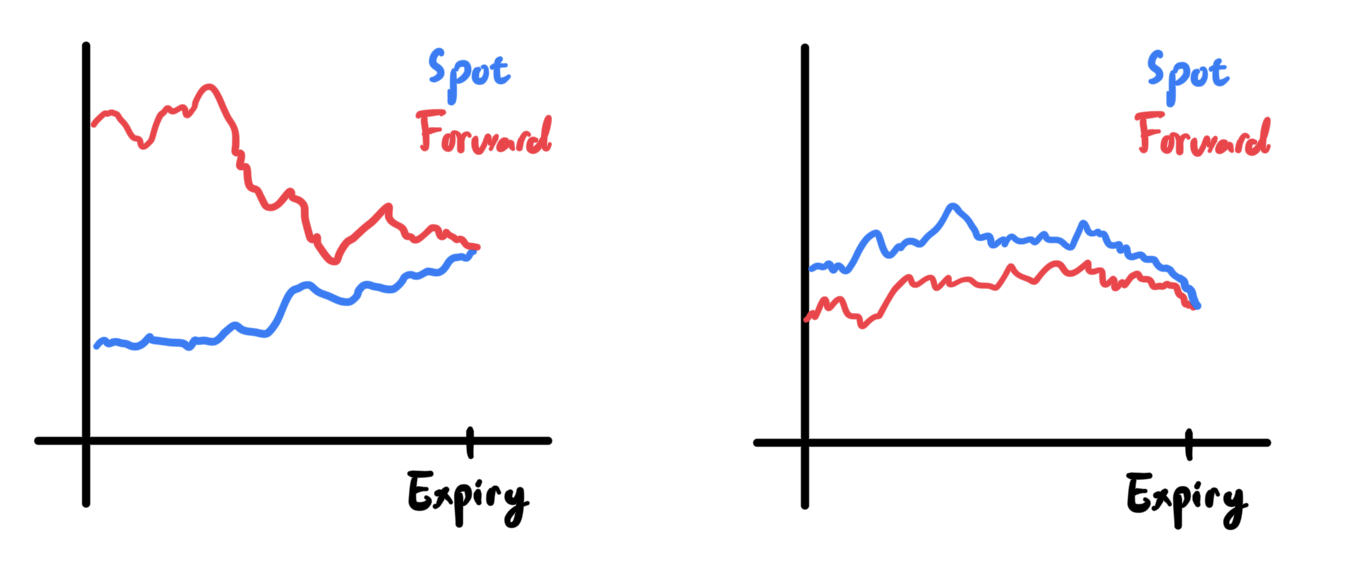
\includegraphics[scale=0.5]{img/cotango_backwardation.png}
        \caption{Spot and future prices must converge upon expiry. If this wasn't the case, then we can construct an arbitrage pairs trade at expiry with the underlying and its forward contract. } 
        \label{fig:cotango_backwardation}
      \end{figure}
    \end{definition}

    \begin{example}[Convergence of Basis Gap]
      It actually isn't the case that the delivery is. 
    \end{example}

    We are still left a little unsatisfied with the futures vs forward price.  To better compare them, we introduce the theorem. 

    \begin{theorem}[Constant Interest Rate]
      If interest rates are constant, then 
      \begin{equation}
        \Phi (t, T) = F(t, T)
      \end{equation}
    \end{theorem}

    \begin{proof}
      
    \end{proof}

    Now what happens if $r$ is not constant? 

    \begin{definition}[Futures Convexity Correction]
      If $S_T$ is positively correlated with the interest rate $r$ (i.e. tends to increase as $r$ increases). If we are long a futures contract, then we receive mark-to-market gains earlier than the forward in environments when interest rates are high, and thus the gains can be invested at a higher rate. Similarly, losses from the long position have to be paid early when rates are low (and thus the future value of the losses is lower). Thus in this case, we would prefer to hold a long futures position relative to a long forward position. Therefore, we have 
      \begin{equation}
        \Phi (t, T) - F(t, T) > 0
      \end{equation}
      which we call the \textbf{futures convexity correction}.
    \end{definition}

    What is the forward price of a futures contract? A futures contract is a forward contract, and it itself should have some fair price.  

    \begin{theorem}[Forward Price of Futures Contract]
      The forward price of a futures contract is the futures price.
    \end{theorem}

    \begin{exercise}[Blyth 5.2]
      Futures on bonds and stocks. 
      \begin{enumerate}
        \item Is the futures price of a fixed rate bond likely to be higher, lower, or the same as its forward price? Give brief reasoning. 
        \item Is the futures price (for a futures contract with maturity $T < T_0$) of a floating rate bond likely to be higher, lower, or the same as its forward price? How does your answer change if $T = T_0$? 
        \item Is the futures price of a stock likely to be higher, lower, or the same as its forward price. 
      \end{enumerate}
    \end{exercise}

  \subsection{Futures on Interest Rates}

\section{Options}

    \begin{definition}[Options]
      An option is a contract that gives the owner the right, but not the obligation, to buy or sell a specific asset. 
      \begin{enumerate}
        \item $T$ is the time until delivery, usually in years. This is fixed per contract and is called the expiration date. 
        \item $K$ is the strike or exercise price. 
        \item $S_t$ is the spot price of the asset at time $t \in [0, T]$. 
      \end{enumerate}
      Since the buyer of the option gains the \textit{right}, not the obligation, the buyer must give some premium. Therefore, a premium changes hands. 
    \end{definition}

    Clearly, this option will have some value, which is estimated by this premium just mentioned, aka the price. 

    \begin{definition}[Value]
      Let $V_K (t, T)$ be the \textbf{true value} of the contract at current time $t \leq T$ of being long an options contract with strike $K$ and maturity $T$. This will vary over time. 

      The \textbf{price} is a noisy estimate of $V_K (t, T)$. Let $C_t$ be the price of a call option and $P_t$ be the price of a put option.
    \end{definition}

    \begin{example}[Option Chain]
      An \textbf{option chain} is a chart that depicts information regarding a class of options. 
      \begin{enumerate}
        \item The top has a list of delivery times: Jun 21, Jul 19, Aug 16, Sep 20, etc. 
        \item For a specific delivery time we have a list of strike prices in the middle, with calls on the left and puts on the right. 
        \item For each strike price and option type we have its market, consisting of a bid/ask prices and their respective sizes, along with the total volume. 
      \end{enumerate}
      \begin{figure}[H]
        \centering 
        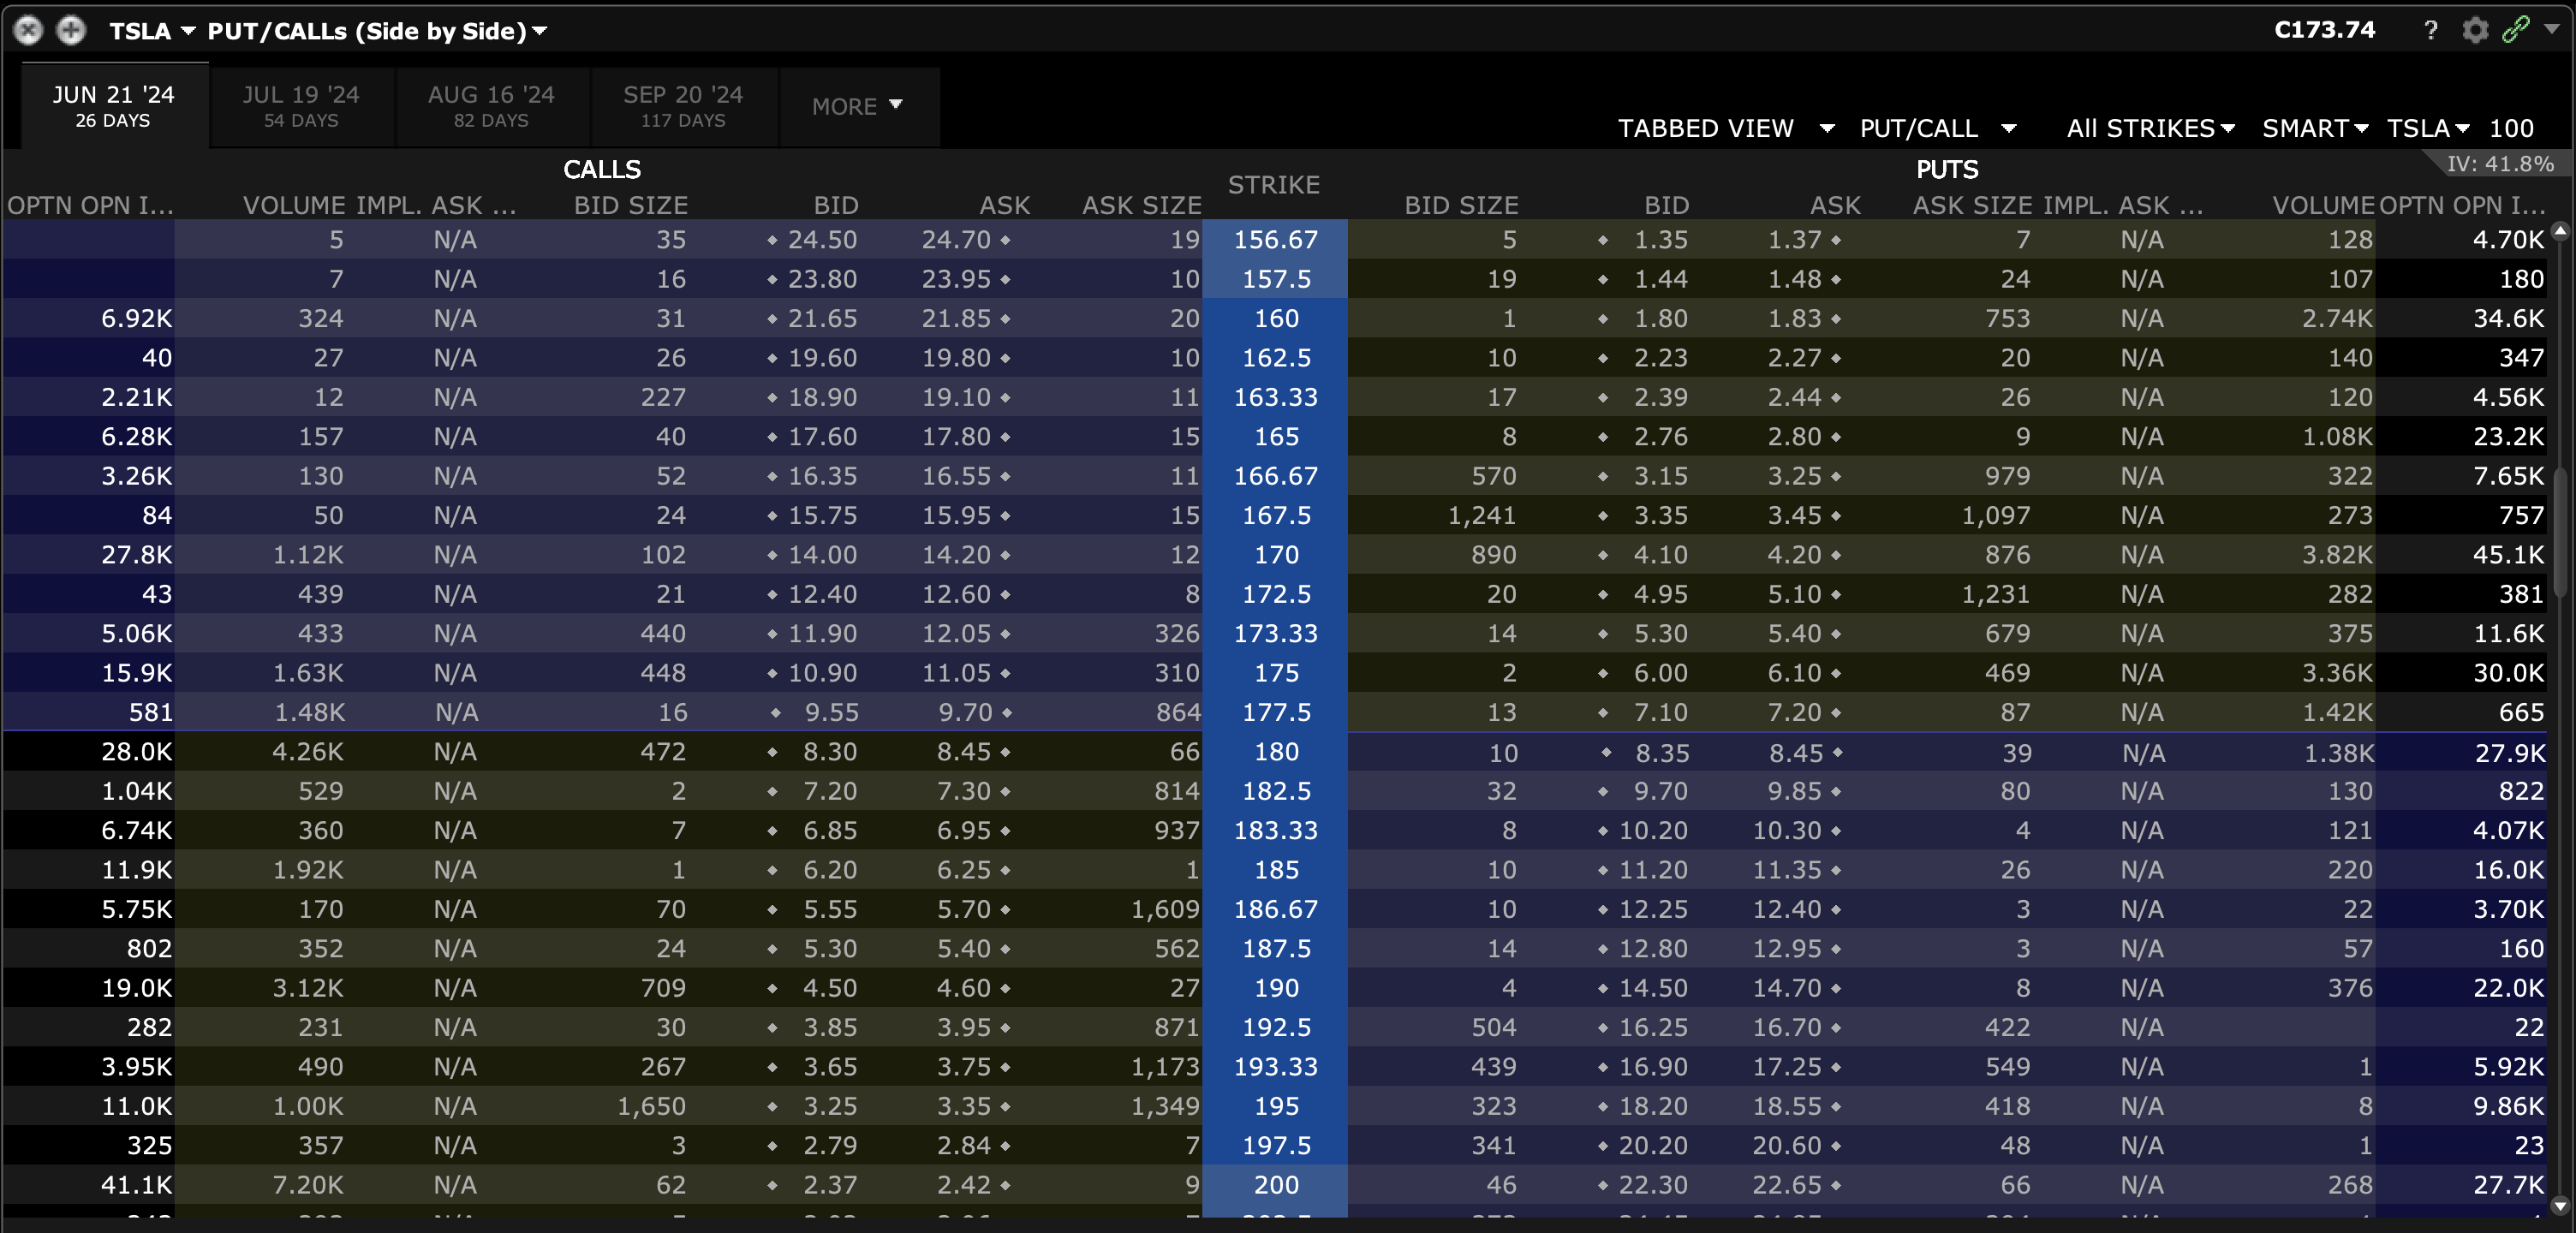
\includegraphics[scale=0.28]{img/option_chain.png}
        \caption{Option chain for TSLA viewed on May 26, 2024 at Interactive Broker's Trader Workstation (TWS). } 
        \label{fig:option_chain}
      \end{figure}
    \end{example}

    To accurately value this, the trader must have a good feel for both the directional movement of the market \textit{and} the timing. A equity trader just needs directional. 

  \subsection{Contract Specifications}

    \subsubsection{Underlying Contracts}

      \begin{example}[Underlying]
        Note that for stock options, a single contract covers 100 shares of the underlying stock. For commmodities, you are really dealing with future options, i.e. options that have an underlying asset of a future contract. 
      \end{example}

      \begin{example}[Company Options]
        Company ABC's shares trade at \$60, and a call writer is looking to sell calls at \$65 with a one-month expiration. If the share price stays below \$65 and the options expire, the call writer keeps the shares and can collect another premium by writing calls again. 

        If the share price appreciates to a price above \$65, referred to as being in-the-money, the buyer calls the shares from the seller, purchasing them at \$65. The call-buyer can also sell the options if purchasing the shares is not the desired outcome.
      \end{example}

    \subsubsection{Settlement}

      Settlement into physical underlying vs settlement into futures vs settlement into cash. 
      Automatic exercise and thresholds for it. 

    \subsubsection{Expiration Date}

    \subsubsection{Exercise}

      There are three types of options. 
      \begin{enumerate}
        \item \textbf{American style} options can be exercised anytime during the life of the option. 
        \item \textbf{European style} options can only be exercised at the expiration date.
        \item \textbf{Bermuda style} options can be exercised at specific dates during the life of the option.
      \end{enumerate}
      This has nothing to do with which continent the options are trading in. It is just a name. Most exchange traded options are American style and most OTC options are European style. Generally, stock and future options tend to be American, and options on indexes tend to be European. 

      Exercise prices are quantized. 

      \begin{example}[Digital Options]
        Options that have a payout of $1$ if a certain event is met and $0$ if else are called \textbf{digital options}. Therefore, it has payout at $T$ 
        \begin{equation}
          \begin{cases} 
            1 & \text{ if } S_T \geq K \\ 
            0 & \text{ if } S_T < K
          \end{cases} 
        \end{equation}
      \end{example}

      \begin{exercise}[Hull 1.16]
        A trader writes (sells) a December put option with a strike price of $\$30$. The price of the option is $\$4$. Under what circumstances does the trader make a profit? 
      \end{exercise}
      \begin{solution}
        Even without a payoff graph, we can see that since I'm selling the option, I'm getting $\$4$. Now, I'm obligated to buy the asset (since it's a put) at $\$30$, and therefore I will profit if the price of the asset is above $\$30$. However, since I already have the cushion of $\$4$, I'm really profiting if the asset price $S_T > 26$. 
        \begin{figure}[H]
          \centering 
          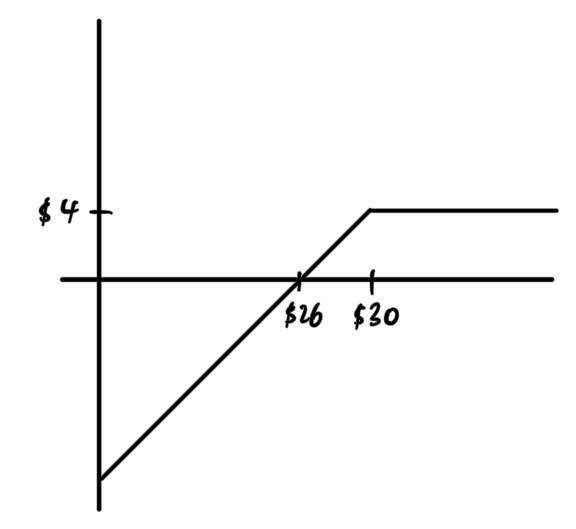
\includegraphics[scale=0.2]{img/ex1-16.png}
          \caption{The payoff graph for the put option from the sellers side.} 
          \label{fig:ex1-16}
        \end{figure}
      \end{solution}

      \begin{exercise}[Hull 1.22]
        I am in a long forward contract and a long put option at the same strike price $K$. What is the payoff of this position at expiration?
      \end{exercise}
      \begin{solution}
        You can simply draw the profit-loss diagram. 
        \begin{figure}[H]
          \centering 
          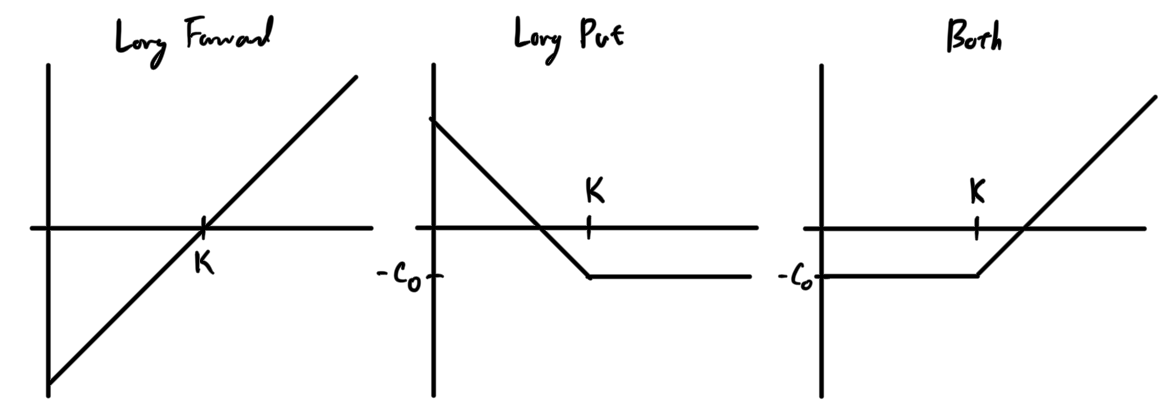
\includegraphics[scale=0.2]{img/ex1-22.png}
          \caption{The payoff graph for the long forward and long put option at the same strike price.} 
          \label{fig:ex1-22}
        \end{figure}
      \end{solution}

      \begin{exercise}[Hull 1.23]
        We have a \textbf{Index Currency Option Note (ICON)} which states the following: 
        \begin{enumerate}
          \item If the exchange rate USD.JPY $ < 169$, then the bond pays $1000$ USD.
          \item If $84.50 \leq USD.JPY \leq 169$, then the bond pays 
            \begin{equation}
              1000 - \max\bigg\{ 0, 1000 \Big( \frac{169}{S_T} - 1 \Big)\bigg\}
            \end{equation}
          \item If $USD.JPY < 84.50$, then the bond pays nothing. 
        \end{enumerate}
        Show that this ICON is a combination of a bond and two options. 
      \end{exercise}
      \begin{solution}
        This seems a bit easy since we can draw the payoff diagram as such. 
        \begin{figure}[H]
          \centering 
          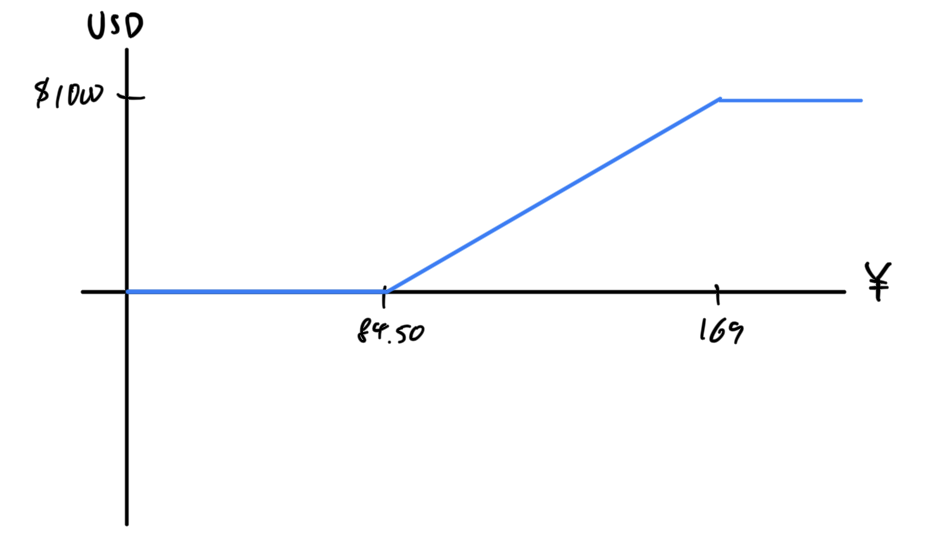
\includegraphics[scale=0.2]{img/ex1-23-1.png}
          \caption{} 
          \label{fig:ex1-23-1}
        \end{figure}
        However, the underlying asset is shown in yen and the payoff in USD, which complicates calculations. You should rather change the underlying to be USD by changing USD.JPY to JPY.USD. Then, we can do some quick sketches to find that you should have a 
        \begin{enumerate}
          \item Bond at $\$1000$. 
          \item Short call at $1/169$ for $\$1000$. 
          \item Long call at $1/84.50$ for $\$1000$.
        \end{enumerate}
        \begin{figure}[H]
          \centering 
          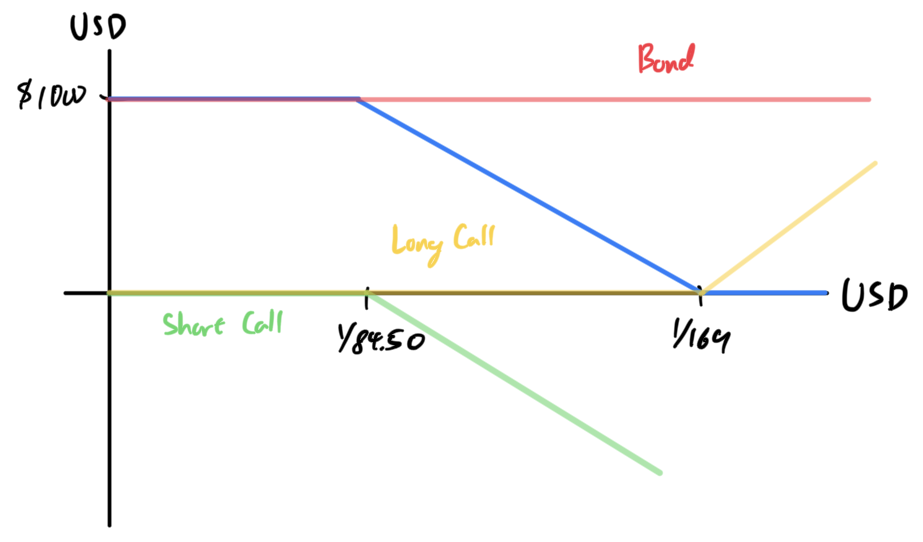
\includegraphics[scale=0.2]{img/ex1-23-2.png}
          \caption{} 
          \label{fig:ex1-23-2}
        \end{figure}
      \end{solution}

  \subsection{Intrinsic Value and Time Premium}

    Let's try to construct some model for this price. The most obvious factor is the difference between the actual price and the strike price, which tells us if our option is currently profitable or not (if we exercised it now). 

    \begin{definition}[Intrinsic Value]
      The \textbf{intrinsic value} is simply what the holder of the option contract would make if they chose to exercise it. That is, for a long call option, it is 
      \begin{equation}
        \IV_K (t, T) = \max\{0, S_t - K\}
      \end{equation}
      and for a long put option, it is 
      \begin{equation}
        \IV_K (t, T) = \max\{0, K - S_t\}
      \end{equation}
      At some time $t$, if the value is positive, then the contract is \textbf{in-the-money (ITM)} or else it is \textbf{out-of-money (OTM)}. If $K = S_t$, then it is \textbf{at-the-money (ATM)}.\footnote{Technically, ATM options are the same at OTM, but as we will see later, ATM options have very specific and desirable characteristics, and such options tend to be the most actively traded. } However, since the strike prices are quantized (e.g. \$65, \$70, \$75, etc.), the contract with strike price closest to the underlying spot is known as the ATM. 
    \end{definition}

    With this, we can already draw \textit{payoff diagrams}, which show the intrinsic value of the option (i.e. the value of the option \textit{at expiry}). 

    \begin{example}[4 Basic Options: Payoff Diagrams at Expiry]
      The 4 basic sides of an option contract are listed below. 
      \begin{enumerate}
        \item If party \textbf{A} buys a call option from party \textbf{B}, then \textbf{A} is in a \textbf{long call} position and has the right to buy at the strike price. \textbf{B} is in a \textbf{short call} position and has the possible obligation to sell at the strike price. 

        \begin{figure}[H]
          \centering 
          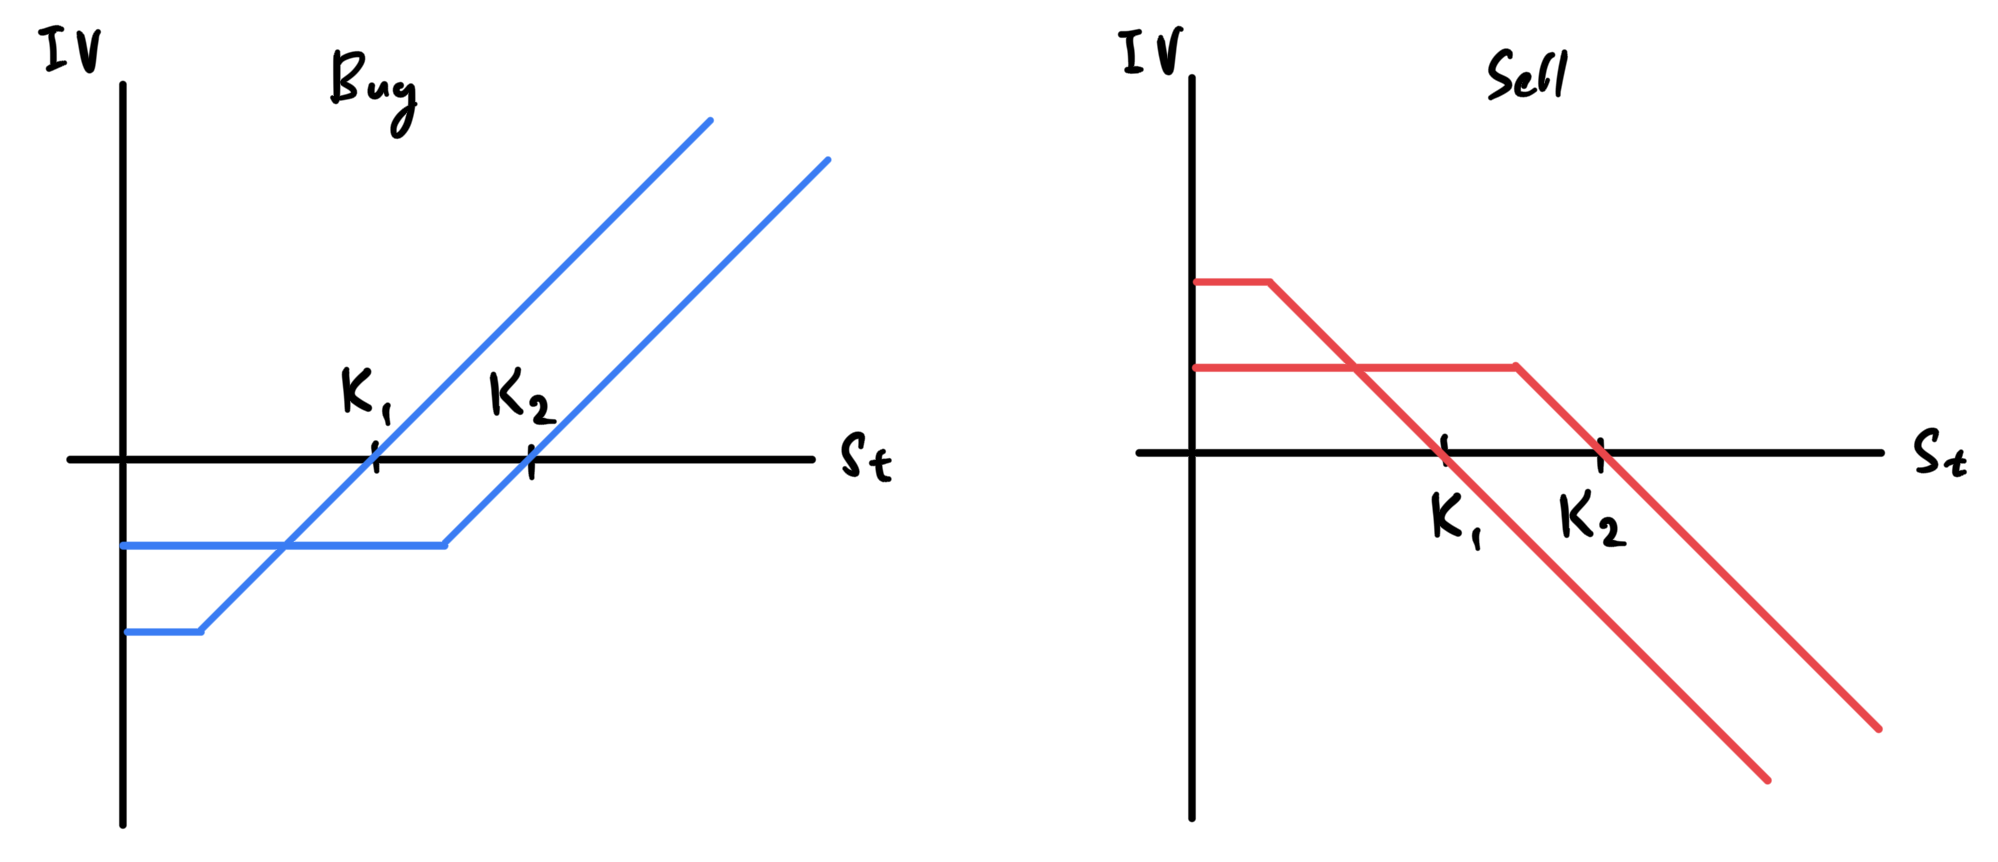
\includegraphics[scale=0.4]{img/call_options.png}
          \caption{For calls, the premium is higher as the strike price gets lower, since you can buy at lower prices. Note that the buyer has limited loss and has unlimited gain with the long put, while the seller has limited gain and unlimited loss with the short put.} 
          \label{fig:call_options}
        \end{figure}

        \item If party \textbf{A} buys a put option from party \textbf{B}, then \textbf{A} is in a \textbf{long put} position and has the right to sell at the strike price. \textbf{B} is in a \textbf{short put} position and has the possible obligation to buy at the strike price. 

        \begin{figure}[H]
          \centering 
          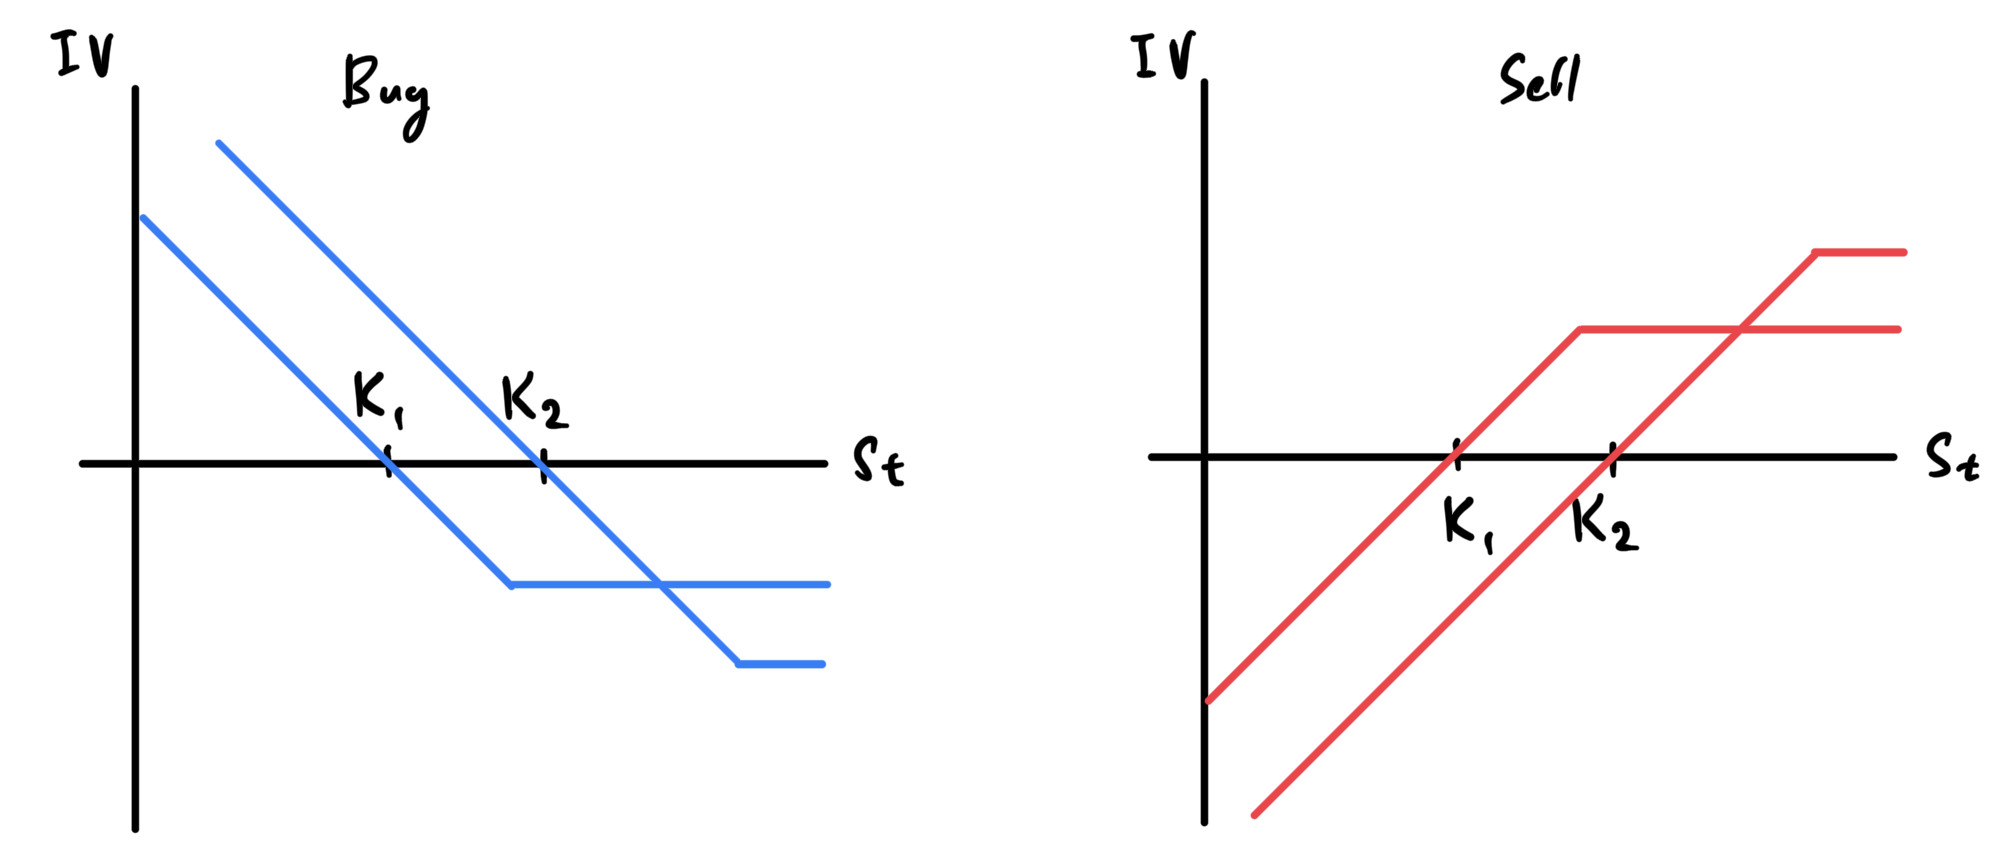
\includegraphics[scale=0.4]{img/put_options.png}
          \caption{For puts, the premium is higher as the strike price is higher, since you can sell at a higher price. Note that the buyer has limited loss and limited gain, and the seller also has limited loss and limited gain. } 
          \label{fig:put_options}
        \end{figure}
      \end{enumerate}

      There are already a few interesting properties. First, note that the long call and short put (like a double negative) take long positions in the underlying, and the other two short positions. 
    \end{example}

    With just the intrinsic value, two options with the same strike price, but with one expiring in 1 month and the other expiring in 6 months, must be worth the same. This is usually not what we see in the market, and the 6-month contract is worth more. Therefore, there is some extrinsic component as well. 

    \begin{definition}[Extrinsic Value]
      The \textbf{extrinsic value} of an option contract $\EV_K(t, t)$ is affected by two components. Traders are willing to pay this additional amount due to some protective characteristics offered by options than an outright long or short equity position. 
      \begin{enumerate}
        \item The \textit{time to expiry}. There is the probability of the underlying asset's price moving in or against our favor during the time remaining. This gives us more \textit{optionality}, i.e. the chance to exercise our option if we choose. 
        \item The \textit{volatility}. This also has to do with the \textit{volatility} of this underlying spot price, which we will talk about later. 
        \item The \textit{distance to ATM}. Having a larger distance to the ATM option means that there is less extrinsic value since the probability of crossing from ITM to OTM or OTM to ITM is smaller. If the option becomes more ITM, then intrinsic value will rise, but if it is more OTM, then the intrinsic value is still $0$ and extrinsic also decreases.  
      \end{enumerate}
      It must clearly satisfy  
      \begin{equation}
        \lim_{t \rightarrow T} \TV_K (t, T) = 0
      \end{equation}
      However, there are times when the time value can be $0$, at which the contract is said to be trading \textbf{at parity}. 
    \end{definition}

    \begin{theorem}[Components of Options Premium]
      The premium paid for an option can be divided into two components, the intrinsic value and the time value. 
      \begin{equation}
        V_K(t, T) = \IV_{K} (t, T) + \TV_K (t, T)
      \end{equation}
      This must satisfy the following. 
      \begin{enumerate}
        \item The time premium must monotonically vanish at $t = T$, i.e. is a \textit{wasting asset}. 
          \begin{equation}
            \lim_{t \rightarrow T} \TV_K (t, T) = 0 \implies \lim_{t \rightarrow T} V_K (t, T) = \IV_K (t, T) 
          \end{equation}
        \item The value of an option with underlying value of $0$ always is also $0$. That is, if $S_T = 0$ (almost surely), then 
          \begin{equation}
            V_K (t, T)  = 0
          \end{equation}
      \end{enumerate}
    \end{theorem}

    To construct a naive model of an option's value that takes into account both the intrinsic value and the time premium, we can first take the expected intrinsic value at expiry.\footnote{This is what Natenberg does in the theoretical pricing models chapter before introducing Black Scholes.} Then, by buying the option for the duration, you are forgoing the opportunity to invest it with interest rate $r$, leading to the \textit{theoretical value}, or the present discounted expected value, of the contract. 
    \begin{equation}
      V_K (t, T) = Z_r (t, T) \mathbb{E} [\IV_K(T, T)]  = \begin{cases} 
        Z_r (t, T) \mathbb{E}_{S_T} [ \max\{S_T - K, 0 \}] & \text{ for calls} \\ 
        Z_r (t, T) \mathbb{E}_{S_T} [ \max\{K - S_T, 0 \}] & \text{ for puts}
      \end{cases}
    \end{equation}
    This makes sense, but it has a severe flaw: it violates the no-arbitrage principle. Let's see how. 

    \begin{example}[Arbitrage Opportunity?]
      Suppose that $S_0 = 50$ and we have 
      \begin{equation}
        \mathbb{P}(S_1 = 40) = \mathbb{P}(S_1 = 70) = \mathbb{P}(S_1 = 110) = \frac{1}{3}
      \end{equation}
      Then, the expected payoff of an option with strike price $60$ that expires at $T = 1$ is 
      \begin{equation}
        \mathbb{E}[\IV_{60} (1, 1)] = \frac{1}{3} \cdot 0 + \frac{1}{3} \cdot 10 + \frac{1}{3} \cdot 50 = 20
      \end{equation}
      Discount this at a rate of say $r = 0.05$ and we have a valuation of \$19. 

      To see how we can construct an arbitrage, let us sell an option for \$19, then borrow an extra \$31, and finally buy the underlying asset. At time $T = 1$, let us consider the following scenarios. 
      \begin{enumerate}
        \item The asset price is $S_1 = 40$. Then, the buyer won't want to exercise. You have the stock, which you sell for \$40, and you pay back the loan of $31 /0.95$, leaving you with $40 - 31 / 0.95 = 7.37$.
        \item The asset price is $S_1 = 70$. Then, the buyer wants to exercise, and you sell the stock for \$60. You are left with $60 - 31 / 0.95 = 27.37$. 
        \item The asset price is $S_1 = 110$. Then, the buyer wants to exercise, and you sell the stock for \$60. You are left with $60 - 31 / 0.95 = 27.37$. 
      \end{enumerate}
      Therefore, this is an arbitrage portfolio since you get riskless profit from nothing. The first reader may find it difficult to find this arbitrage as if it was pulled from thin air. Later on, we will explore how this arbitrage opportunity is even found, and it turns out that the error in this derivation comes from the assumption of the probability distribution itself; it is not a risk neutral measure. 
    \end{example}
  
  \subsection{Put Call Parity}
    
    Before we start developing more options theory, let us talk about a simple property of options. This states that one long call and one short put equals one long forward, all at the same strike $K$ and expiry $T$. The naive argument is that if you look at the payoff graphs, you can see that it is true. 

    \begin{figure}[H]
      \centering 
      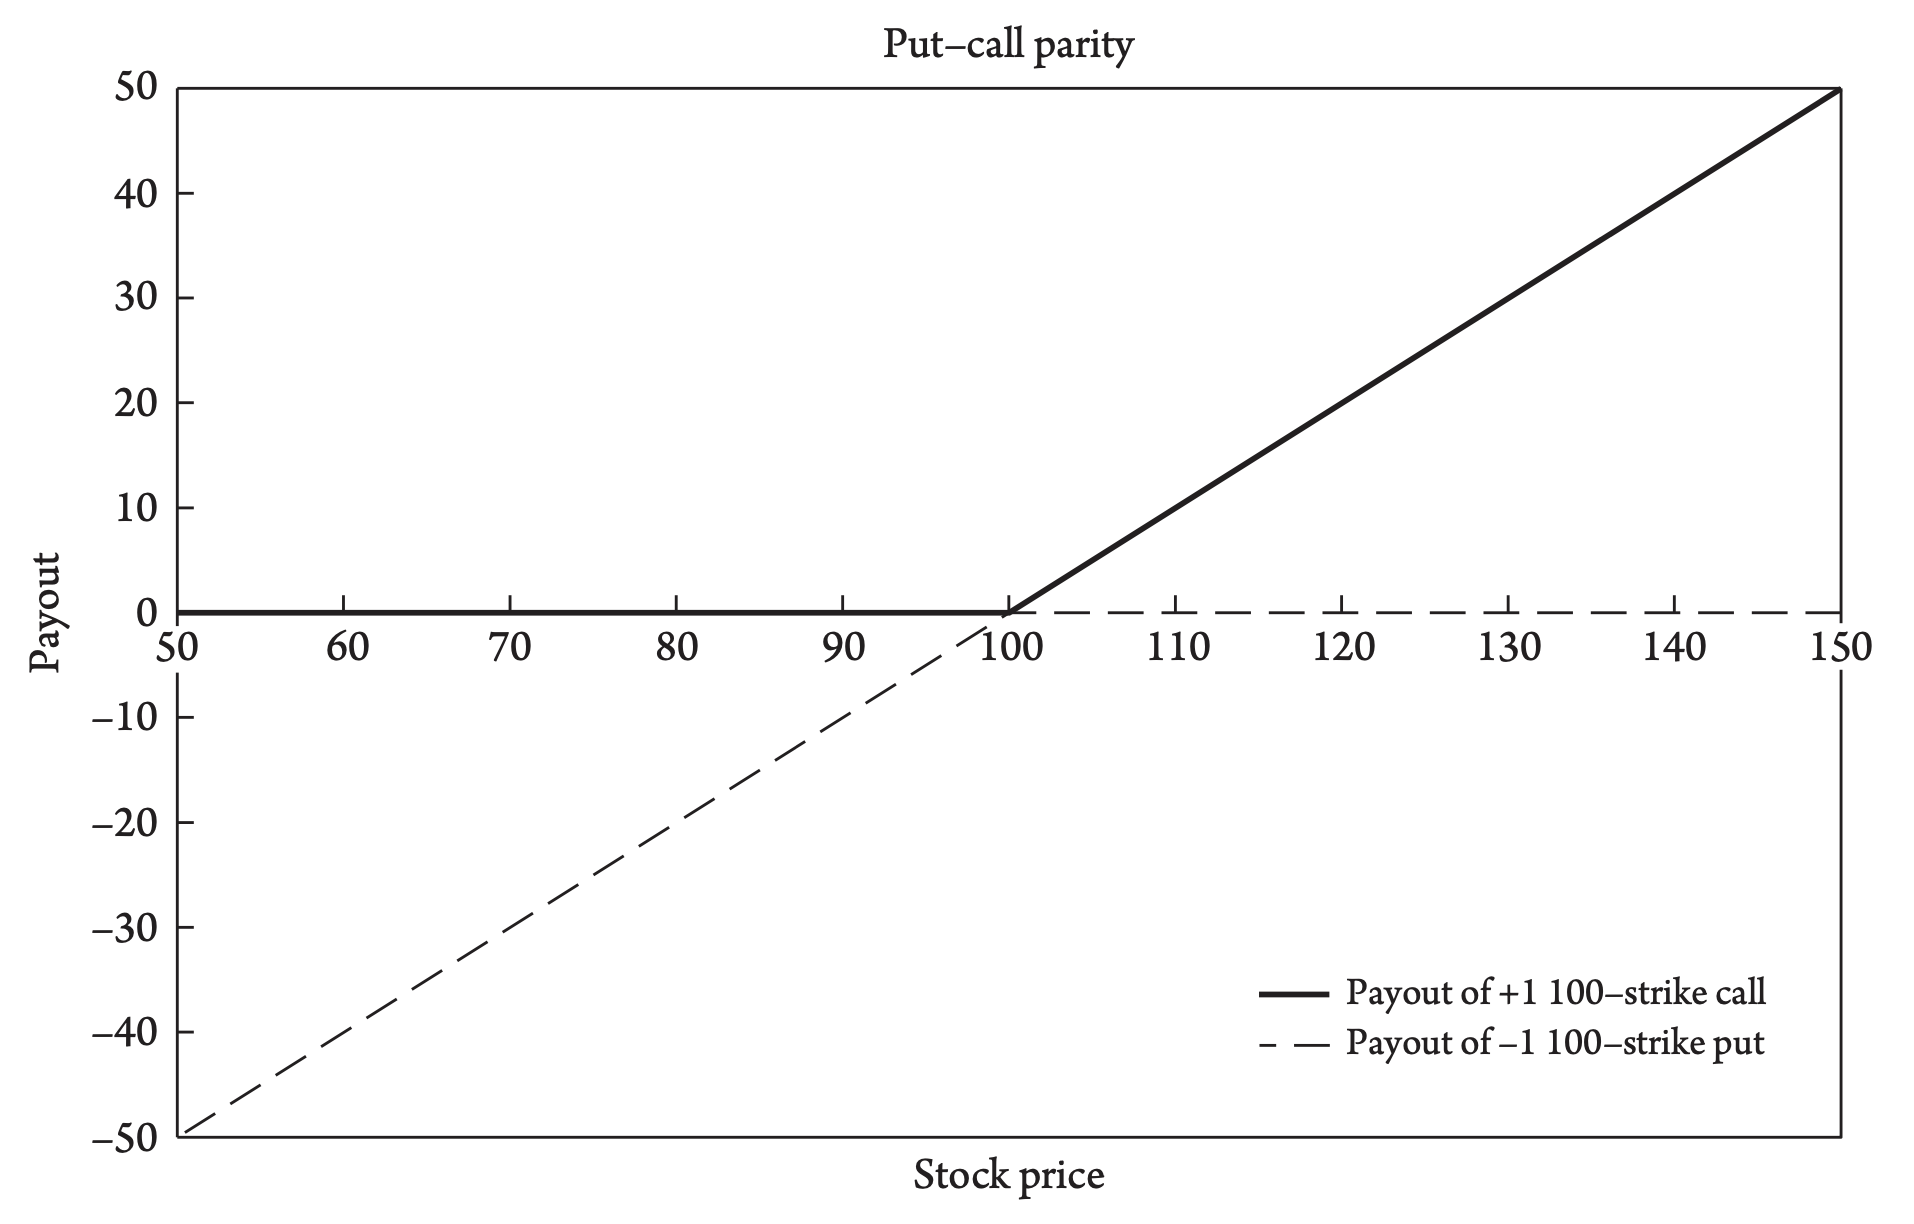
\includegraphics[scale=0.32]{img/put_call_parity.png}
      \caption{Adding the payoff graphs of the two options position at expiry shows that the position is equal to a forwards position at expiry. } 
      \label{fig:put_call_parity}
    \end{figure}

    However, this is not the correct argument, since this result is only true \textit{at expiry}. Fortunately, we have the (corollary of the) monotonicity theorem that tells us that if the portfolios are equal with probability $1$ at some point in time, it is equal at all points in time. This is the general argument we will use here.\footnote{Without even knowing the formula for the pricing of these options, like Black Scholes, it is amazing that we can still prove this relationship. } 

    \begin{lemma}[Put-Call Parity]
      The prices of the put and call option of the same strike price are related to the value of a forward option by 
      \begin{align}
        C_K (t, T) - P_K (t, T) & = V_K (t, T) \\ 
                                & = (F(t, T) - K) Z(t, T)
      \end{align}
      In the specific case where interest rates are $0$, then we can simplify notation and write\footnote{I like to use the mnemonic of the S\&P to realize that $S_t$ and $P$ must be on the same side.}
      \begin{equation}
        C - P = S_t - K \iff C + K = S_t + P 
      \end{equation}
    \end{lemma}
    \begin{proof}
      Say that you are long call and short put with common strike $K$ and expiry $T$. Then, this is the same thing as having a forward contract. Therefore, 
      \begin{equation}
        C_K (t, T) - P_K (t, T) = V_K (t, T)
      \end{equation}
    \end{proof}

    An immediate consequence of this is that is the delivery price $K = F(t, T)$ we have by definition $V_K (t, T) = 0$ and therefore 
    \begin{equation}
      C_{F(t, T)} (t, T) = P_{F(t, T)} (t, T)
    \end{equation}
    That is, these \textbf{at the money forward (ATMF)} options have the same price, which holds despite any distributional assumptions. 

    \begin{theorem}
      An ITM call option or put should never be worth less than its intrinsic value. 
    \end{theorem}
    \begin{proof}
      We have 
      \begin{equation}
        C_t = S_t - K e^{-rt} + P_t > S_t - K e^{-r t} > S_t - K
      \end{equation}
    \end{proof}


    \begin{theorem}[Bounds on Call Prices]
      We have 
      \begin{equation}
        \max\{0, S_t - K Z(t, T)\} \leq C_K (t, T) \leq S_t
      \end{equation}
    \end{theorem}

    \begin{corollary}
      The price of an American call and European call on a non-dividend paying stock are equal. 
    \end{corollary}

  \subsection{Calls are Puts and Puts are Calls}

    There is a duality between calls and puts. In fact, it is possible to turn one into the other by either longing or shorting the underlying. There may be terminology differentiating a covered call and a protective call, but there are really two instruments. When we say we are \textit{longing} a covered call/put, we are longing the option and then hedging with the appropriate underlying. 

    \begin{definition}[Covered Call, CV-C]
      A long \textbf{covered call} is a long call and a short underlying, which is equivalent to a long put. 
      \begin{center}
        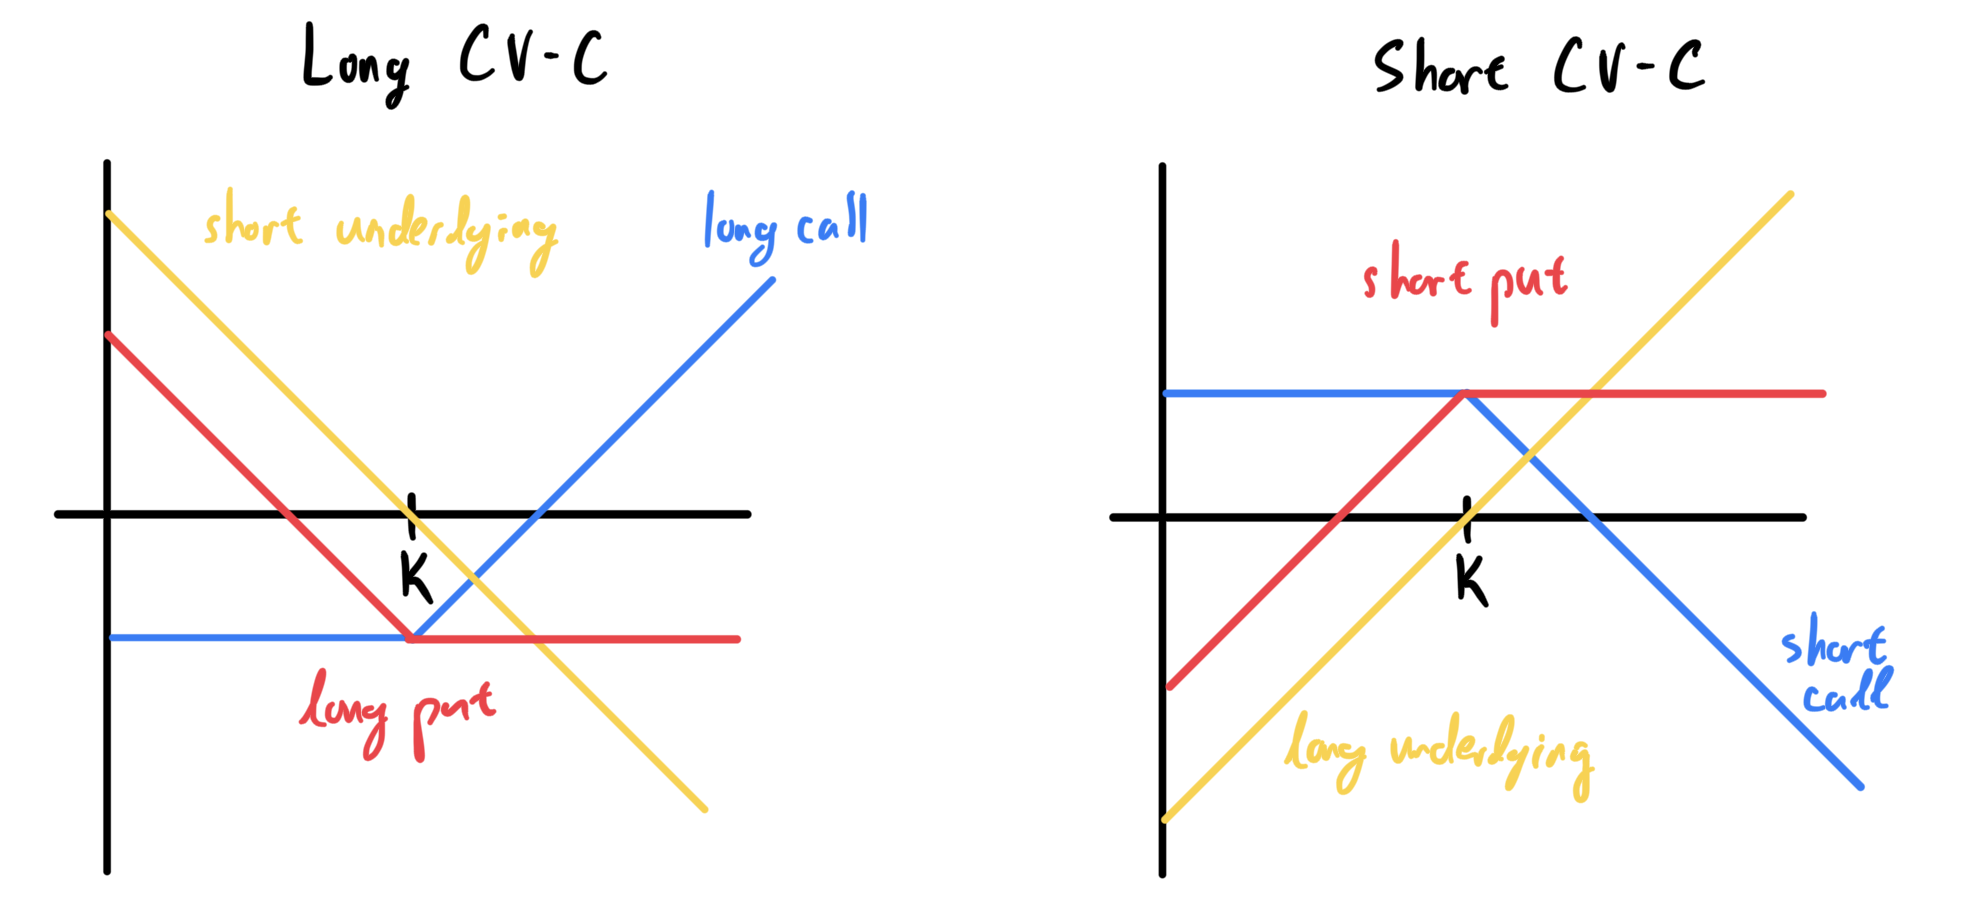
\includegraphics[scale=0.3]{img/covered_call.png}
      \end{center}
    \end{definition}

    \begin{definition}[Covered Put, CV-P]
      A long \textbf{covered put} is a long put and a long underlying, which is equivalent to a long call. 
      \begin{center}
        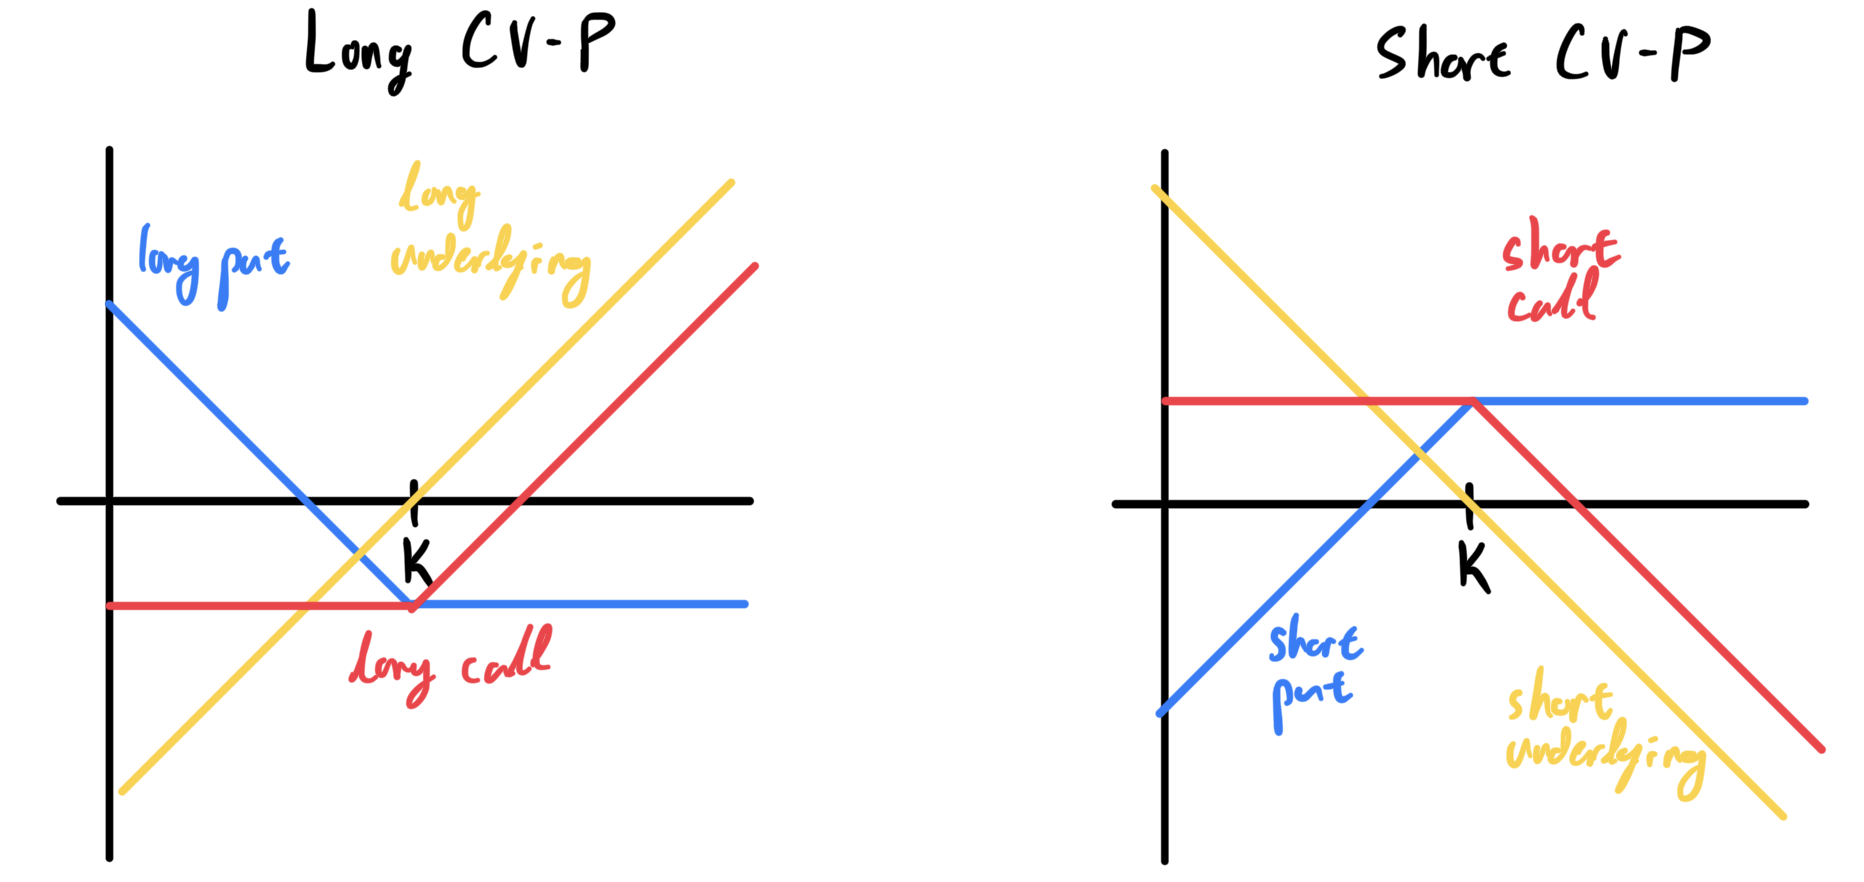
\includegraphics[scale=0.3]{img/covered_put.png}
      \end{center}
    \end{definition}

    While it is worthwhile to draw the payoff diagrams at first, it is good to remember that if we own a covered call, we are taking an opposite position of a put (so must be a long put). 

    This means that we can also take two options at the same strike and delivery and use them to make a pure long or pure short position in the underlying. These are called \textit{synthetic} long and short positions. 

    \begin{definition}[Synthetic Long/Short]
      A \textbf{synthetic long} is to buy a (long call + short put) position. A \textbf{synthetic short} is to buy a (short call + long put) position. 
      \begin{center} 
        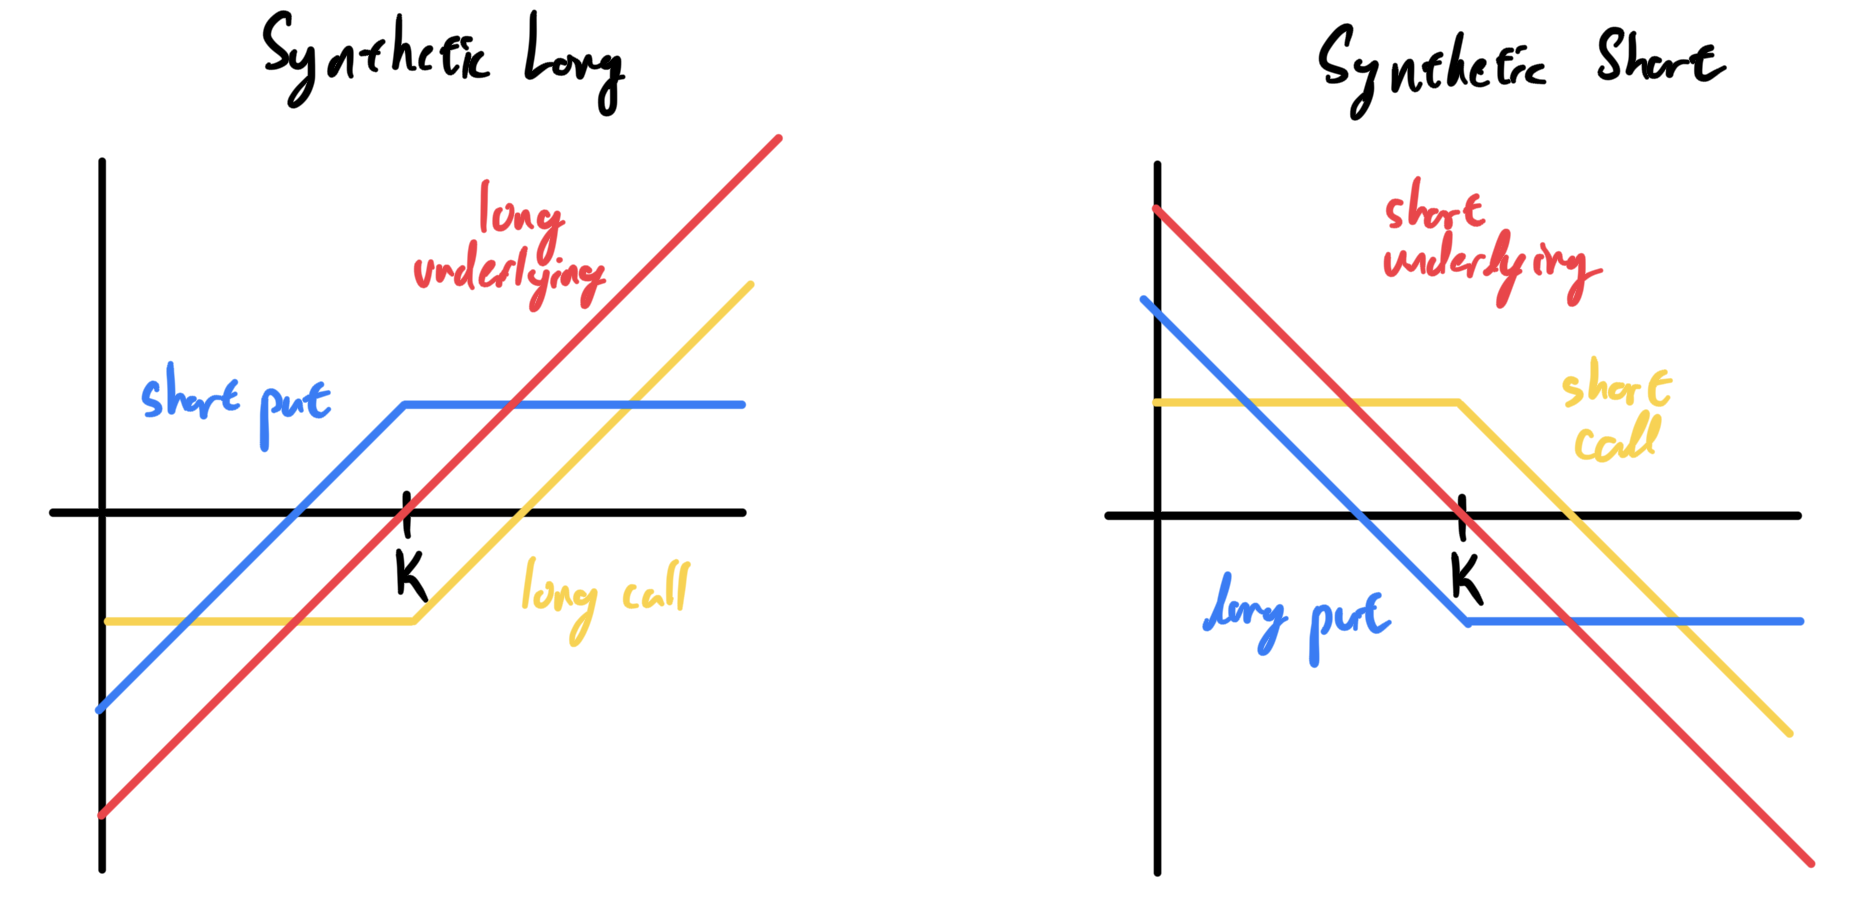
\includegraphics[scale=0.3]{img/synthetic_long_short.png}
      \end{center}
      Clearly, selling a synthetic long is buying a synthetic put, and the two are counterparties to each other. 
    \end{definition}

    If they are so equivalent, then what is the actual difference? There are two main points that we consider: 
    \begin{enumerate}
      \item The exchange fees of trading two securities is obviously greater than one, so covered options and synthetic longs/shorts are more expensive. However, they are also sold together in a package as \textit{combinations}, or \textit{combos}, so this can be avoided. 
      \item Trading these combos is safer, since you are guaranteed to make both trades simultaneously. On the other hand, if you attempt to buy a call and a sell an underlying, the price that you want it executed may not go through during the second that you attempt to buy the second security. Therefore you must buy and sell combos together always.\footnote{For example, consider that we bought a straddle and the market collapsed, we might want to take off the call and let the put "ride". What usually happens is that then the market will rally and you lose on both the call and the put. }
      \item As a market maker accrues positions in various options and underlyings, it may be simpler to analyze our positions using these combos rather than all at once. If we own a short put and a covered call, it is simpler to think of this as a short put and a long put, which has a flat payoff diagram (assuming same strike and expiry). 
    \end{enumerate}

  \subsection{Straddles and Strangles}

    \begin{definition}[Straddles, Y]
      A \textbf{long straddle} is achieved when you buy a call option and a put option at the same strike price $K$ and expiration date, and it is a long volatility position. If you bought the call for price $C_t$ and bought the put at price $P_t$, then we have the following properties: 
      \begin{enumerate}
        \item \textit{Value}. This is worth $C_t + P_t$. 
        \item \textit{Profit Lower Bound}. The most you can lose is $C_t + P_t$, the value of the straddle.  
        \item \textit{Positive Profit}. You profit if the stock moves at least $C_t + P_t$ away from the strike. If $S_T \not\in [K - (C_t + P_t), K + (C_t + P_t)]$, then we profit. 
        \item This is generally not a directional bet so you would buy ATM options, where $C_t = P_t$, but this does not always need to be the case. 
      \end{enumerate}
      \begin{center}
        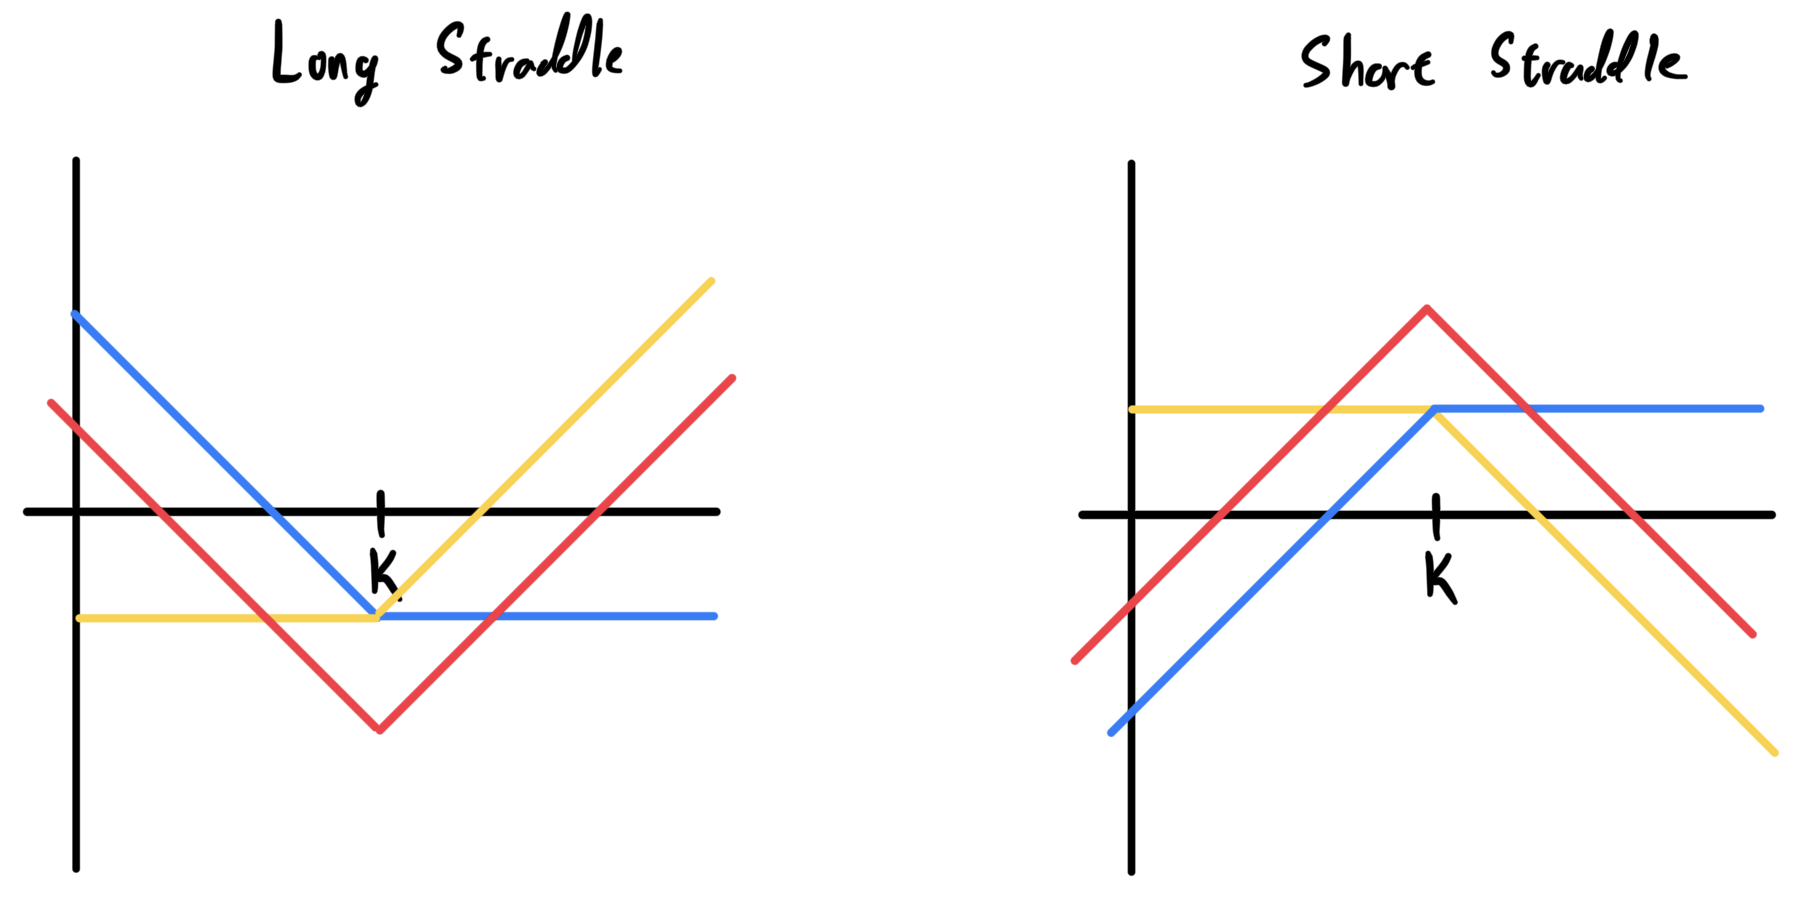
\includegraphics[scale=0.3]{img/straddle.png}
      \end{center}
    \end{definition}

    \begin{definition}[Strangles]
      A \textbf{long strangle} is achieved when you buy a call and a put option at \textit{different} strike prices $K_c$ and $K_p$ (usually both out-of-money) and the same expiration date, and it is a long volatility position. If you bought a call option for price $C_t$ and bought the put at price $P_t$, then we have the following properties: 
      \begin{enumerate}
        \item \textit{Value}. This is worth $C_t + P_t$. 
        \item \textit{Profit Lower Bound}. The most you can lose is again $C_t + P_t$, the value of the strangle. However, since they are both out of the money, you pay less premium than you would do on a straddle. 
        \item \textit{Positive Profit}. You profit if the stock moves at least $C_t + P_t$ to the left of the put strike $K_p$ or moves at least $C_t + P_t$ to the right of the call strike. 
        \item This is generally not a directional bet so you would buy ATM options, where $C_t = P_t$, but this does not always need to be the case. 
      \end{enumerate}
      \begin{center}
        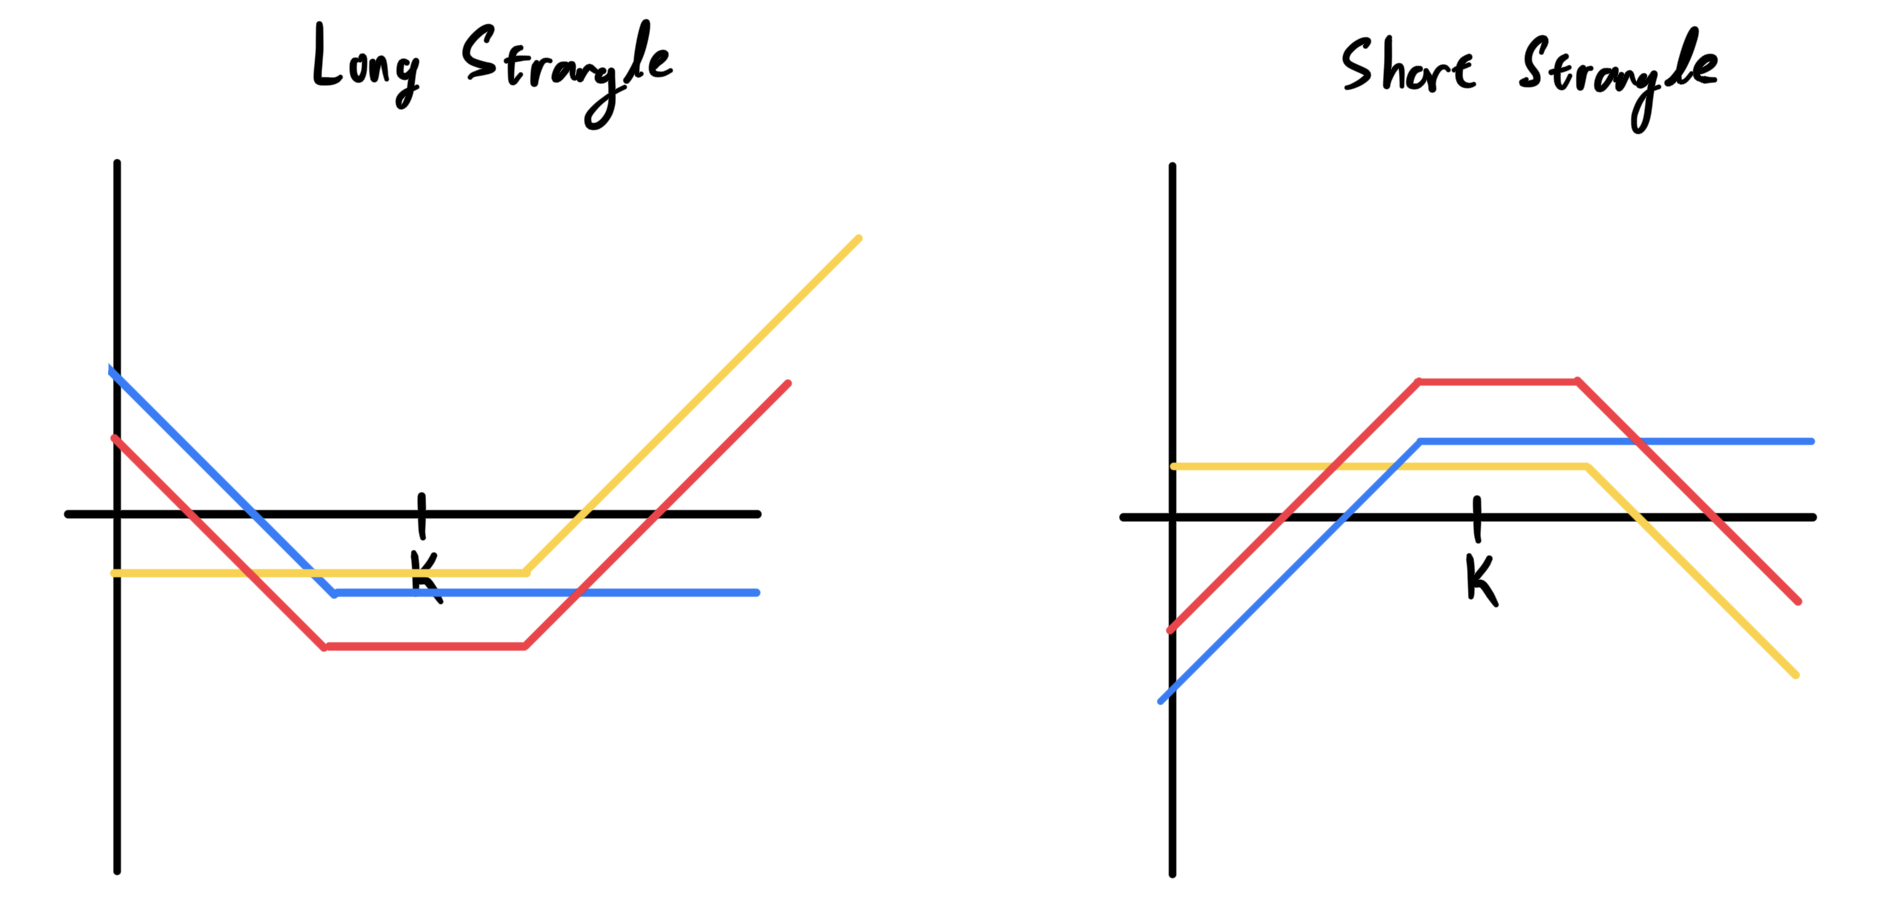
\includegraphics[scale=0.3]{img/strangle.png}
      \end{center}
    \end{definition}

    The following fact quantifies the differences between the straddle and the strangle. 

    \begin{theorem}[Gammas of Straddles and Strangles]
      The straddle will always have a higher gamma than the strangle and therefore will be more appropriate for traders who are betting on an increase in the actual volatility of the market. 
    \end{theorem}

  \subsection{Call, Put, and Box Spreads}

    \begin{definition}[Call Spread, CS]
      A \textbf{call spread} consists of a long call with smaller strike $K_1$ and a short call on a larger strike of $K_2$.\footnote{It is also called a bull call spread since you are betting directionally that it will go up.} It has the following properties. 
      \begin{enumerate}
        \item \textit{Value}. The $K_1$ strike option will be worth more since it has a lower strike, so the total value of this is $C_1 - C_2 > 0$. 
        \item \textit{Profit Lower Bound}. The most you can lose is if they are both OTM, meaning that you just lose what you paid for, which is $C_2 - C_1$. 
        \item \textit{Profit Upper Bound}. The most you gain is if they are both ITM, meaning you gain $-(C_1 - C_2) + (K_2 - K_1)$. 
        \item The longer the spread ($K_2 - K_1$) is, the more you stand to gain, but the premium on the $K_2$ call will be more smaller compared to that of the $K_1$, meaning you have more to lose. 
      \end{enumerate}
      \begin{center}
        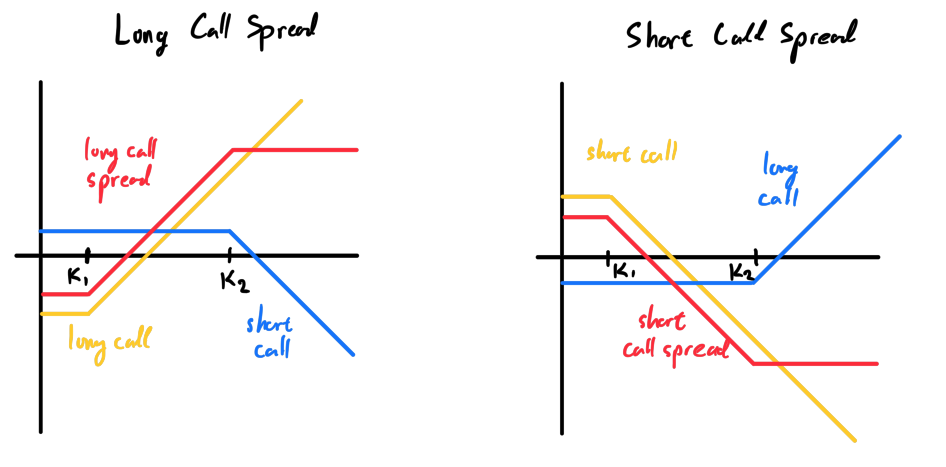
\includegraphics[scale=0.3]{img/call_spread.png}
      \end{center}
    \end{definition}

    \begin{definition}[Put Spread, PS]
      A \textbf{put spread} consists of a short put with smaller strike $K_1$ and a long put with a larger strike $K_2$.\footnote{It is also called a bear put spread since you are betting directionally that the underlying will go down. } It has the following properties. 
      \begin{enumerate}
        \item \textit{Value}. The $K_2$ strike option will be worth more since it has a higher strike, so the total value of this is $P_2 - P_1 > 0$. 
        \item \textit{Profit Lower Bound}. The most you can lose is if they are both OTM, meaning that you just lose what you paid for, which is $P_2 - P_1 > 0$
        \item \textit{Profit Upper Bound}. The most you can gain is if they are both ITM, meaning you gain $-(P_2 - P_1) + (K_2 - K_1)$
      \end{enumerate}
      Often, the theo of a put spread is shown as positive, but 
      \begin{center}
        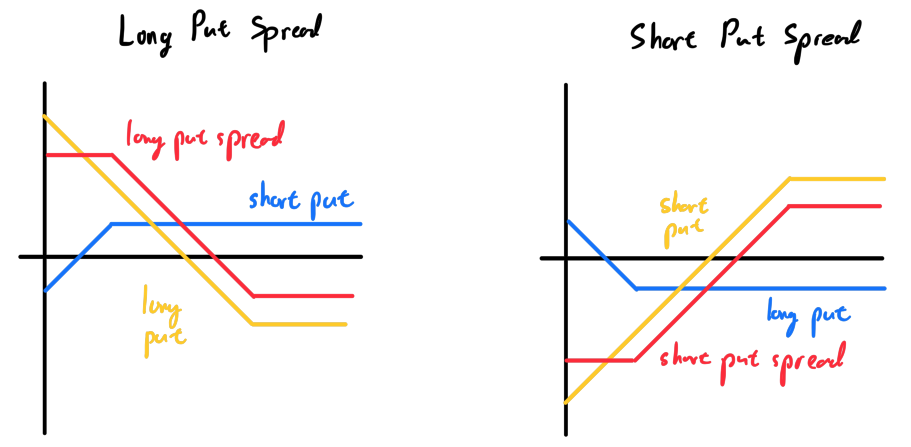
\includegraphics[scale=0.3]{img/put_spread.png}
      \end{center}
    \end{definition}

    \begin{theorem}[Upper Bound on Value Call Spread]
      A call spread can never be worth more than the difference between the strikes. 
    \end{theorem}
    \begin{proof}
      Say $K_2 > K_1 \implies P_2 > P_1$. Then 
      \begin{equation}
        \begin{cases}  C_1 & = S_t - K e^{-rt} + P_1 \\ C_2 & = S_t - K e^{-rt} + P_2 \end{cases} \implies C_1 - C_2 = (K_2 - K_1) e^{-rt} + (P_1 - P_2) 
      \end{equation}
      and since the larger strike put is worth more, the expression above is less than $(K_2 - K_1) e^{-rt} < K_2 - K_1$. 
    \end{proof}

    With this, we can construct an approximation of the value of a call spread right when the underlying price is at the midpoint of the two strikes. 

    \begin{corollary}[Call Spread Value at Midpoint]
      Given a $K_1/K_2$ call spread, if the underlying $S_t = (K_1 + K_2)/2$, then the value of the call spread is 
      \begin{equation}
        C_1 - C_2  = \frac{K_2 - K_1}{2}
      \end{equation}
    \end{corollary}

    Using the theorem above, along with put call parity, we can use this to approximate options prices on an option chain, a process known as \textbf{rough opening}. 

    \begin{definition}[Box Spread, ]
      A \textbf{box spread} consists of a long call spread and a long put spread. It is essentially buying all 4 types of options. This is quite weird, since by PCP, it should just be a net $0$ (in fact, net negative if we look at exchange fees). However, as a market maker, we can quote around this theo to lock in an instant profit, i.e. an arbitrage. 
      \begin{center}
%        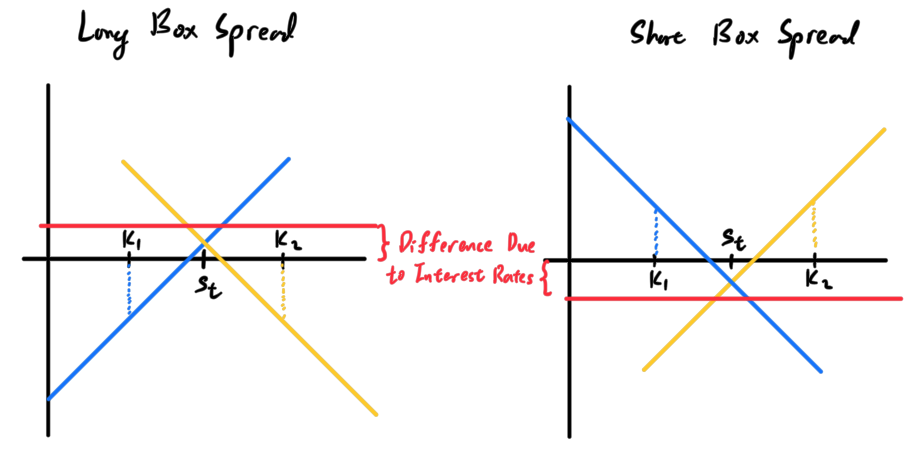
\includegraphics[scale=0.3]{img/box_spread.png}
      \end{center}
    \end{definition}

  \subsection{Butterfly Spreads}

    Conservative traders who do not like the unlimited risk associated with shorting options can use a butterfly spread to limit their loss potentials. It is a short volatility strategy that makes money from volatility decreasing but mostly from time decay. We can construct butterfly spreads with long calls, long puts, short calls, and short puts, but we will only introduce long calls here. 

    \begin{definition}[Call Butterfly Spread]
      A \textbf{long call butterfly spread} consists of a long call with strike $K_1$, 2 short calls with strike $K_2$, and long call with strike $K_3$, where $K_1 < K_2 < K_3$. It can also be considered a short straddle (shorting volatility) and a long strangle (hedging large movements). It is a short volatility bet with the following properties: 
      \begin{enumerate}
        \item \textit{Value}. The value of this spread is $C_1 - 2C_2 + C_3$. 
        \item \textit{Profit Lower Bound}. The most you can lose is the price that you paid for the spread, which is $C_1 - 2C_2 + C_3$. 
        \item \textit{Profit Upper Bound}. The most you can earn is if $S_T$ is at $K_2$, which is $K_2 - K_1$. We must subtract the cost of this spread as well. 
        \item We usually have the middle call be ATM so that we are direction neutral. 
        \item We usually employ a \textit{symmetrical butterfly} where $K_2 - K_1 = K_3 - K_2$ due to some nice properties mentioned later. 
      \end{enumerate}

      \begin{center}
        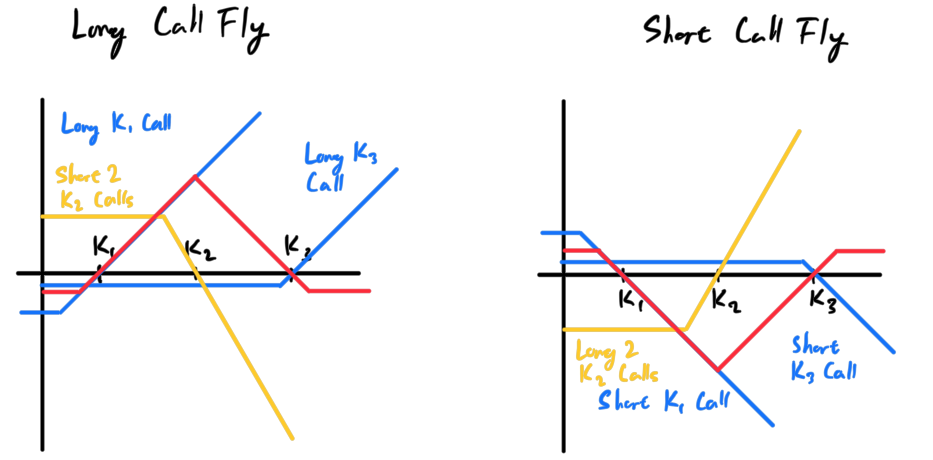
\includegraphics[scale=0.35]{img/call_fly.png}
      \end{center}
    \end{definition}

    \begin{theorem}[Call and Put Butterflies]
      Notice that a symmetrical call butterfly spread is the same as a put butterfly spread. This should be quite intuitive since the payoff diagrams of the butterflies are symmetrical across the Y-axis. However, we can actually prove it using put-call parity.
    \end{theorem}
    \begin{proof}
      Let $C_i$ and $P_i$ have the same expiry and strike $K_i$. Then, by PCP, 
      \begin{align*}
        C_1 - 2 C_2 + C_3 & = (P_1 + S_t - K_1) - 2 (P_2 + S_t - K_2) + (P_3 + S_t - K_3) \\ 
                          & = P_1 - 2 P_2 + P_3 - K_1 + 2 K_2 - K_3
      \end{align*} 
      and since it is symmetrical, the strikes vanish.
    \end{proof}

    \begin{theorem}[Value of Fly]
      The value of a symmetrical fly spread can never be less than $0$. 
    \end{theorem}
    \begin{proof}
      The most you can lose is $C_1 - 2C_2 + C_3 = 0$, so it is bounded below by $0$ and it must be greater. 
    \end{proof}

    They are also brilliant from a time decay standpoint, especially in the last 30 days. They decay at an extraordinary rapid pace in the last 30 days. So these trades are ideal to reap the rewards of heavy time decay without having to assume an unreasonable amount of risk. 

    \begin{definition}[Iron Butterfly Spread]
      An \textbf{iron butterfly spread} consists of a short call 
    \end{definition}

    The greeks of a long call fly and a short iron fly are the same since they are translationally invariant, but their theos are not. 

    \begin{theorem}
      The theos of iron and call butterflies sum to the differences of their strikes. 
    \end{theorem}

  \subsection{Risk Reversals}

    \begin{definition}[Risk Reversal, RR]
      A long \textbf{risk reversal} consists of a short put on lower strike $K_1$ and a long call on higher strike $K_2$. It is called a risk reversal since if you are shorting an underlying, you can long a RR to reverse your risk and hedge it (note that this is equivalent to a put spread). 
      \begin{center}
        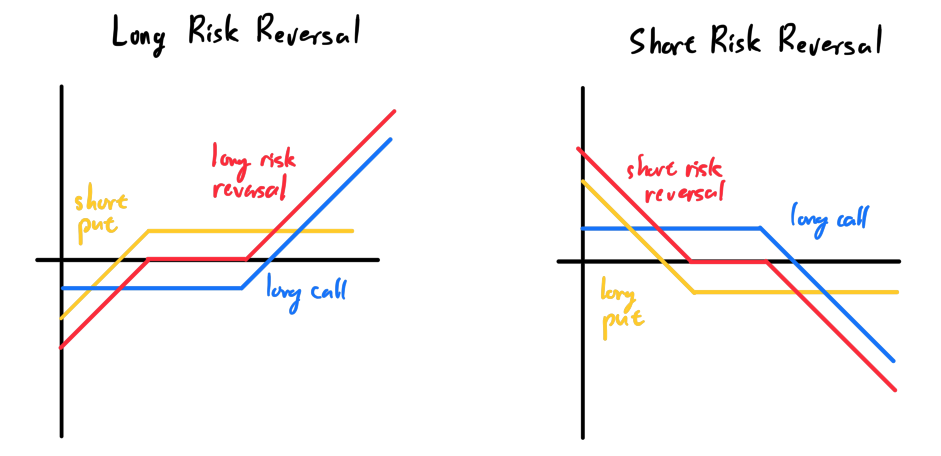
\includegraphics[scale=0.3]{img/risk_reversal.png}
      \end{center}
      Notice that in risk reversals, either the call or the put could have higher premium. It is important to know which one. 
      \begin{enumerate}
        \item If the call has a higher premium, you say a $K_1/K_2$-risk reversal, \textit{call over}. To clarify out position, we say the delta, e.g. $+52$ delta (if long) or $-48$ delta (if short).  
        \item If the put has a higher premium, you say a $K_1/K_2$ RR, \textit{put over}, $\Delta$ delta. 
      \end{enumerate}
    \end{definition}

    To make markets on risk reversals, you take theos of lower strike puts and higher strike calls. 

  \subsection{Conversion Reversals}

    \begin{definition}[Conversion, Reversal]
      
    \end{definition}

  \subsection{Ratio Spreads and Ladders}

    \begin{definition}[1x2 Call Spread]
      A \textbf{1 by 2} consists of buying one $K_1$ call and selling two $K_2$ calls. 
    \end{definition}

    \begin{definition}[Call, Put Ladder]
      A \textbf{put ladder} consists of selling a $K_1$ put, selling a $K_2$ put, and buying a $K_3$ put where $K_1 < K_2 < K_3$. 
    \end{definition}

\section{Black Scholes}

  \subsection{Risk-Neutral Probability}

    Let's consider a simple model on a non-dividend paying stock at price \$100 at time $t = 0$. Assume annually compounded interest rates are 10\% and that 
    \begin{equation}
      \mathbb{P}(S_1 = 120) = p, \;\; \mathbb{P}(S_1 = 90) = 1 - p
    \end{equation}
    That is, it either increases by 20\% or decreases by 10\%, these events labeled $A$ and $B$. Let's try to value these options using 2 different ways. 
    \begin{enumerate}
      \item Assume that we long an option. Then, the payoff at time $T$ would be 
        \begin{equation}
          \max\{S_T - 110, 0\} = \begin{cases}
            10 & \text{ with prob.} = p \\ 
            0 & \text{ with prob.} = 1 - p 
          \end{cases} 
        \end{equation}
        Therefore, our expected payoff is $10p$, which we discount to get $10p Z(0, 1)$. Note from before that this method of valuation is inherently faulty. 

      \item Assume that we long an option and short $\Delta$ stock. Then, the payoff at time $T$ would be 
        \begin{equation}
          \max\{S_T - 110, 0\} - S_T \Delta = \begin{cases} 
            10 - 120 \Delta & \text{with prob. } = p  \\ 
            - 90\Delta & \text{ with prob. } = 1 - p
          \end{cases} 
        \end{equation}
        Let's minimize the variance of this portfolio by setting the two equal to each other. 
        \begin{equation}
          10 - 120 \Delta = -90 \Delta \implies \Delta = \frac{1}{3}
        \end{equation}
        Therefore, let's consider this portfolio of long one option and short $1/3$ stock. Then, our profit is 
    \end{enumerate}

    What would our exposure be if we held various options? Say that we bought a call at strike $110$. Then, our payout would be 

    Say that we shorted a call option at strike $110$. Then, our payout would be 
    \begin{equation}
      - \max\{ S_T - 110, 0 \} = \begin{cases} 
        -10 & \text{ with prob.} = p \\ 
        0 & \text{ with prob.} = 1 - p 
      \end{cases}
    \end{equation}
    This gives us negative exposure\footnote{There would be a premium that we would receive when we sold the option, but for now we assume that we just hold it. } and to hedge this, we may consider holding a position in the underlying stock. Let's say we want to hold $\Delta$ positions of the stock. Then, our payout at time $T$ is 
    \begin{equation}
      S_T \Delta - \max\{S_T - 110, 0\} = \begin{cases} 
        120 \Delta - 10 & \text{with prob. } = p  \\ 
        90\Delta & \text{ with prob. } = 1 - p
      \end{cases} 
    \end{equation}
    If we wanted to minimize the variance of this portfolio, then we can just solve for 
    \begin{equation}
      120 \Delta - 10 = 90 \Delta \implies \Delta = \frac{1}{3} 
    \end{equation}
    This is called a \textit{covered call}.\footnote{It is nice to remember that for calls, you take the opposite position in the underlying (e.g. buy calls, sell underlying) and for puts, you take the same position (e.g. buy puts, buy underlying). } We can develop these for hedges against the four basic options. 

    Recall our initial attempt at pricing options using the discounted expected payoff. In fact, let's redo this with the current example to gain some insight on how one would find this arbitrage. Assume that the asset price is $S_0$ and that we have a one-step binomial model with 
    \begin{equation}
      \mathbb{P}(S_1 = S_0 (1 + u)) = p \text{ and } \mathbb{P}(S_1 = S_0 (1 - d)) = 1 - p
    \end{equation}
    Let the strike price be $K$, which should be  

  \subsection{Continuous Time Limit and Log Normal Distribution}

    Limit of this risk neutral binomial goes to log normal, which is fundamental assumption of Black Scholes. 

  \subsection{Continuous Time Limit and Derivation}

    The binomial tree is a good initial model, but clearly the values that a stock can take are not a set of discrete numbers. It is more mathematically convenient to take the limit of this tree to the reals. 

    \begin{question}[TBD]
      Show that the risk neutral probability converges to the log normal distribution. 
    \end{question}

    The problems are modeled through the Black-Scholes model comes in, which is stated with the following PDE.

    \begin{definition}[Black Scholes PDE]
      The \textbf{Black-Scholes PDE} is the following. 
      \begin{equation}
        \frac{\partial V}{\partial t} + \frac{1}{2} \sigma^2 S^2 \frac{\partial^2 V}{\partial S^2} + r S \frac{\partial V}{\partial S} - rV = 0
      \end{equation}
    \end{definition}

    We can model the price of a stock and want to construct a measure that follows this stochastic differential equation. 
    \begin{equation}
      dS_t = \mu S_t dt + \sigma S_t dW_t
    \end{equation}
    under some real world measure $\mathbb{P}$. This is equivalent to 
    \begin{equation}
      \frac{d S_t}{S_t} = \mu dt + \sigma d W_t \text{ where } dt = (dW_t)^2
    \end{equation}
    We first start off with the intuitive pricing of a call option as a discounted expected payoff. 
    \begin{equation}
      C_0 = \mathbb{E} [ e^{-r T} \max\{ S_T - K, 0\}]
    \end{equation}
    In Black Scholes, there is a formula like this, but not under the real world measure $\mathbb{P}$, but this is true under another measure $\mathbb{Q}$.  This is formalized in the following theorem. 

    \begin{theorem}[Girsanov Theorem]
      There exists another measure $\mathbb{Q} \sim \mathbb{P}$ s.t. 
      \begin{equation}
        dS_t = r S_t dt + \sigma S_t \Tilde{W}_t 
      \end{equation}
      where $\Tilde{W}_t$ is another Brownian motion. 
    \end{theorem}

    Let's go back to the main point. We want to solve this SDE to get geometric Brownian motion. 

    \begin{theorem}[Solution to SDE]
      It turns out that the solution is 
      \begin{equation}
        S_t = S_0 \exp \bigg\{ \bigg( r - \frac{1}{2} \sigma^2 \bigg) t + \sigma \Tilde{W}_t \bigg\}
      \end{equation}
    \end{theorem}
    \begin{proof}
      Using Ito's lemma, we have 
      \begin{align}
        d (\ln S_t) & = \frac{1}{S_t} dS_t - \frac{1}{S_t^2} \cdot \frac{1}{2} (d S_t)^2 \\ 
                    & = r dt + \sigma d \Tilde{W}_t - \frac{1}{2} \sigma^2 dt \\
                    & = \bigg( r - \frac{1}{2} \sigma^2 \bigg) dt + \sigma d \Tilde{W}_t
      \end{align}
      and so 
      \begin{equation}
        [ \ln S_T ]_0^T = \int_0^T \big( r - \frac{1}{2} \sigma^2 \big) \,dt + \int_0^T \sigma d\Tilde{W}_t \implies \ln \bigg( \frac{S_T}{S_0} \bigg) = \bigg( r - \frac{1}{2} \sigma^2 \bigg) T + \sigma (\Tilde{W}_T - \Tilde{W}_0)
      \end{equation}
      and since $\Tilde{W}_0 = 0$ since it is Brownian motion, we have the result. 
    \end{proof}

    Now we just need to calculate $C_t = \mathbb{E} [ e^{-r T} \max \{S_T - K, 0\}]$, where only $S_T$ is random. Since we just found a solution to $S_T$ above, which has the only random component $\Tilde{W}_T$, this distribution is related to Brownian motion $\Tilde{W}_T$. Note that 
    \begin{equation}
      \ln \bigg( \frac{S_T}{S_0}\bigg) = \underbrace{\bigg( r - \frac{1}{2} \sigma^2 \bigg) T}_{\text{mean or normal}} + \underbrace{\sigma}_{\text{std. dev.}} \Tilde{W}_T \implies \ln \bigg( \frac{S_T}{S_0} \bigg) \sim \mathcal{N} \Big( \big( r - \frac{1}{2} \sigma^2 \big) T, \sigma^2 \Big) 
    \end{equation}
    since $\Tilde{W}_T$ already is a normal with mean $0$ and variance $T$. Now we can calculate the integral/expectation. The max term is annoying to deal with, so we divide it 
    \begin{align}
      C_T & = \mathbb{E}_{\mathbb{Q}} [ e^{-rT} (S_T - K) \, \mathbbm{1} (S_T > K)] \\
          & = e^{-r T} \big\{ \mathbb{E}_{\mathbb{Q}}[S_T \, \mathbbm{1} (S_T > K)] - \mathbb{E}_{\mathbb{Q}} [K \, \mathbbm{1}(S_T > K)] \big\} \\
          & = e^{-r T} \big\{ \mathbb{E}_{\mathbb{Q}}[S_T \, \mathbbm{1} (S_T > K)] - K \mathbb{P}(S_T > K) \big\}
    \end{align}
    We can already see that each of these expectations evaluate to each term in the Black Scholes solution. Let's solve the simpler second term first. We have 
    \begin{align}
      \mathbb{P}(S_T > K) & = \mathbb{P} \big( \ln(S_T / S_0) > \ln(K / S_0) \big) \\
                          & = \mathbb{P} \bigg( \underbrace{\frac{\ln(S_T / S_0) - (r - \frac{1}{2} \sigma^2) T}{\sigma \sqrt{T}}}_{N(0, 1)} > \frac{\ln(K /S_0) - (r - \frac{1}{2} \sigma^2) T}{\sigma \sqrt{T}} \bigg)  \\
                          & = \mathbb{P} \bigg( \underbrace{\frac{\ln(S_T / S_0) - (r - \frac{1}{2} \sigma^2) T}{\sigma \sqrt{T}}}_{N(0, 1)} < \frac{\ln(S_0/K) + (r - \frac{1}{2} \sigma^2) T}{\sigma \sqrt{T}} \bigg)  \\
                          & = \Phi \bigg( \frac{\ln(S_0 /K) + (r - \frac{1}{2} \sigma^2) T}{\sigma \sqrt{T}} \bigg)
    \end{align}
    As for the second expectation, since $S_T = S_0 e^{\ln (S_T / S_0)}$, we can substitute $X = \ln (S_T / S_0)$ and write 
    \begin{align}
      \mathbb{E}_{\mathbb{Q}} [S_T \, \mathbbm{1} (S_T > K)] & = \mathbb{E} [S_0 e^X \, \mathbbm{1} (S_0 e^X > K)] \\
                                                             & = S_0 \mathbb{E} [ e^X \mathbbm{1}(X > \ln (K/S_0))] \\
                                                             & = S_0 \int_{\ln(K/S_0)}^\infty e^x \frac{1}{\sqrt{2 \pi} b} e^{-\frac{(x - a)^2}{2 b^2}} \,dx \\
                                                             & = S_0 \int_{\ln(K/S_0)}^\infty e^{rT} \, N(a + b^2, b^2) \,dx \\ 
                                                             & = S_0 e^{rT} \, \Phi \bigg( \frac{\ln(S_0 /K) + (r + \frac{1}{2} \sigma^2) T}{\sigma \sqrt{T}} \bigg)
    \end{align}
    where $a = \big( r - \frac{1}{2} \sigma^2 \big) T$ and $b = \sigma \sqrt{T}$. Therefore, by substituting these into the original expectation, we have 
    \begin{align}
      C_T & = e^{-rT} \bigg\{ S_0 e^{rT} \, \Phi \bigg( \frac{\ln(S_0 /K) + (r + \frac{1}{2} \sigma^2) T}{\sigma \sqrt{T}} \bigg) - K \Phi \bigg( \frac{\ln(S_0 /K) + (r - \frac{1}{2} \sigma^2) T}{\sigma \sqrt{T}} \bigg) \bigg\} \\
          & = \Phi \bigg( \frac{\ln(S_0 /K) + (r + \frac{1}{2} \sigma^2) T}{\sigma \sqrt{T}} \bigg) \, S_0 - \Phi \bigg( \frac{\ln(S_0 /K) + (r - \frac{1}{2} \sigma^2) T}{\sigma \sqrt{T}} \bigg) K e^{-r T}
    \end{align}

  \subsection{Properties}

    It has the following solution, which we will state now but will elaborate later. 

    \begin{definition}[Black-Scholes Option Pricing Formula]
      Given a call option, the \textbf{Black-Scholes} pricing formula states that 
      \begin{equation}
        V_K (t, T) = \mathcal{B}_t (K, T - t, S_t, r, \sigma) = \Phi(d_1) S_t - \Phi (d_2) K e^{-r (T - t)}
      \end{equation}
      where $r$ is some risk-free applicable interest rate, $\Phi$ is the normal CDF, $\sigma$ is the volatility of the underlying, and 
      \begin{equation}
        d_1 = \frac{\ln (S_t / K) + \big( r + \frac{\sigma^2}{2}\big) (T - t)}{\sigma \sqrt{T - t}} \text{ and } d_2 = d_1 - \sigma \sqrt{T - t}
      \end{equation}
    \end{definition}

    Black-scholes also allows us to draw payoff diagrams for time $t$ that is not necessarily at expiry, known as \textit{risk diagrams}. This allows us to see the value of these options both at different spot prices of the underlying and at different points in time. 

    \begin{figure}[H]
      \centering
      \begin{subfigure}[b]{0.48\textwidth}
      \centering
        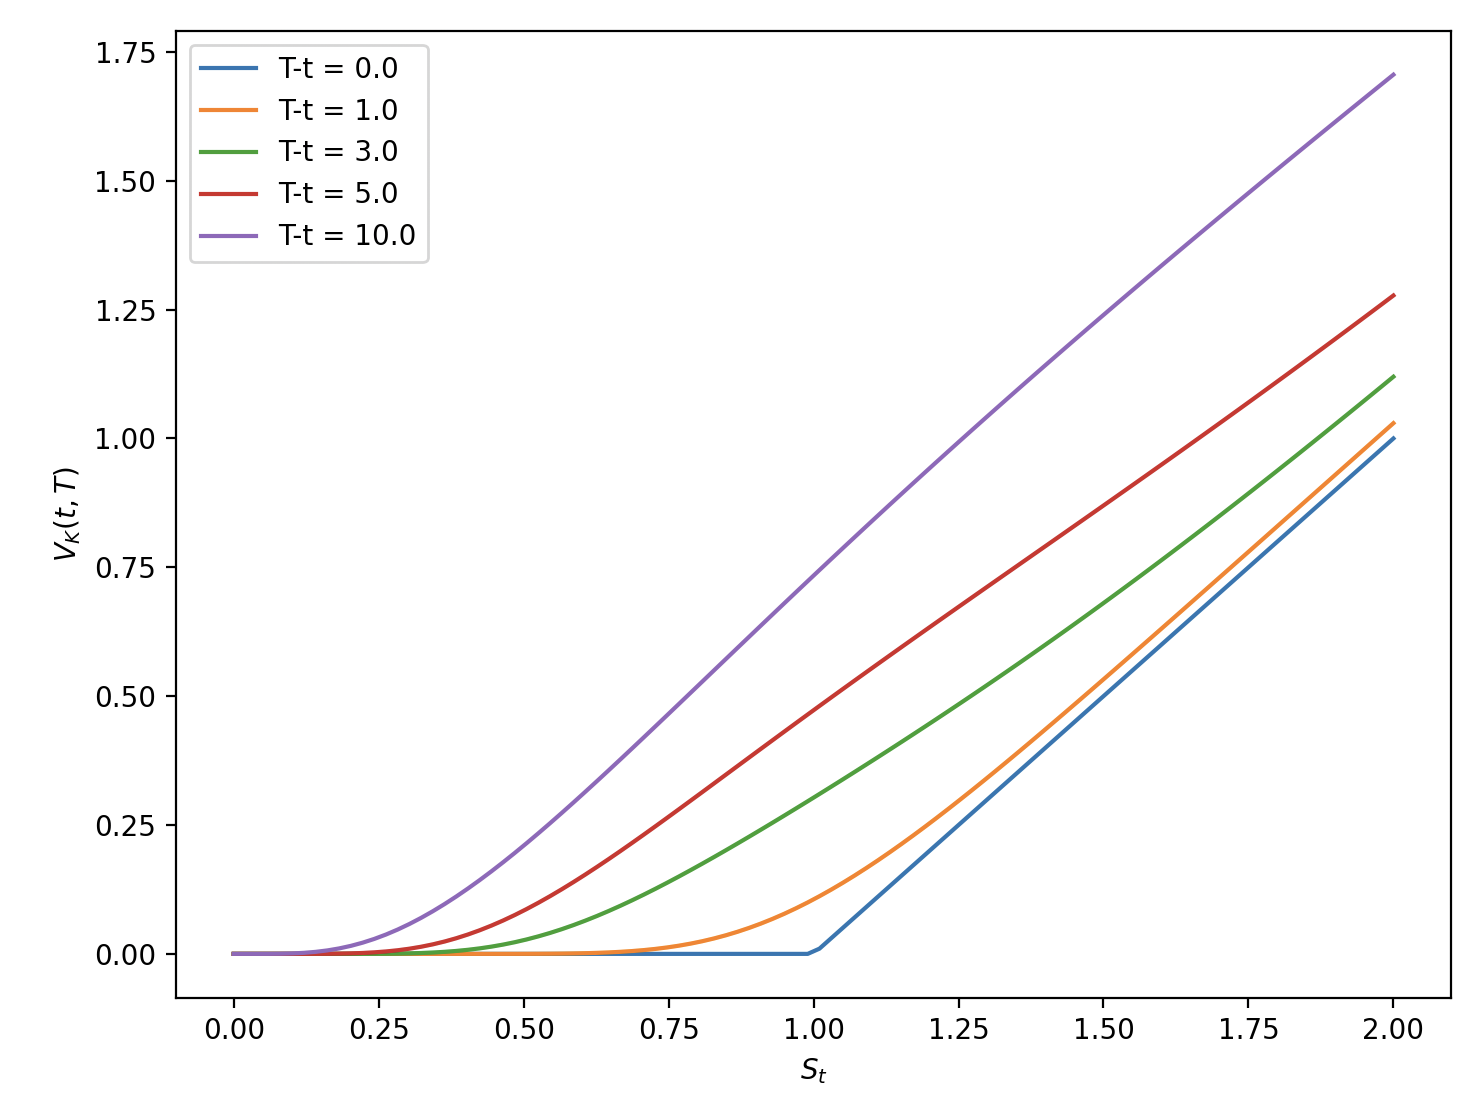
\includegraphics[width=\textwidth]{img/value_graph_over_time.png}
        \caption{The value graphs of European options over time according to Black Scholes model. }
        \label{fig:value_graph_over_time}
      \end{subfigure}
      \hfill 
      \begin{subfigure}[b]{0.48\textwidth}
      \centering
        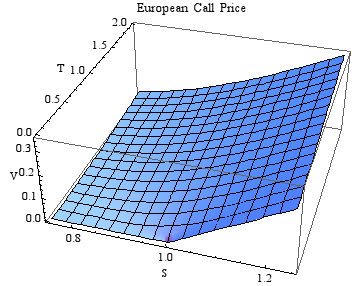
\includegraphics[width=\textwidth]{img/option_surface.png}
        \caption{3D surface. }
        \label{fig:option_surface}
      \end{subfigure}
      \caption{}
      \label{fig:option_pricing_graphs}
    \end{figure}
    
    \begin{figure}[H]
      \centering 
      \begin{lstlisting}
        import numpy as np 
        import math
        from scipy.stats import norm
        import matplotlib.pyplot as plt 

        def blackScholes(K:float, T_t:float, S_t:float, r:float, sigma:float) -> float: 
            d1 = (np.log(S_t / K) + (r + (sigma ** 2)/2) * (T_t)) / (sigma * math.sqrt(T_t))  
            d2 = d1 - sigma * T_t 
            return norm.cdf(d1) * S_t  - norm.cdf(d2) * K * math.e ** (-r * T_t)

        K = 1.0 
        r = 0.03
        sigma = 0.23
        X = list(np.linspace(0, 2, 100))
        for T_t in [0., 1., 2., 3.]: 
            Y = []
            for S_t in X: 
                Y.append(blackScholes(K, T_t, S_t, r, sigma))
            plt.plot(X, Y, label=f"{T_t}")
        plt.show() 
      \end{lstlisting}
      \caption{Code snippet used to generate graphs.} 
      \label{fig:black_scholes_graph_code}
    \end{figure}

    \begin{exercise}[Talking with Friends]
      What does the price of a call option go to as the volatility of the underlying goes to infinity? Describe it mathematically and heuristically.\footnote{A discussion can be found \href{https://quant.stackexchange.com/questions/39490/value-of-call-option-as-volatility-goes-to-infinity}{here}. } 
    \end{exercise}

    \begin{solution}[Talking with Friends]
      We can simply take this limit of the Black Scholes formula as $\sigma \rightarrow \infty$. Note that 
      \begin{align}
        \lim_{\sigma \rightarrow \infty} d_1 = + \infty & \implies \Phi(d_1) = 1 \\ 
        \lim_{\sigma \rightarrow \infty} d_2 = - \infty & \implies \Phi(d_2) = 0
      \end{align}
      and by plugging it in we get 
      \begin{equation}
        \lim_{\sigma \rightarrow \infty} V_K (t, T) = S_t 
      \end{equation}
      This means that it would converge onto the spot price of the stock. Let's now describe this more heuristically. It is clear that the value of a call option will increase as the upside of the option is greater if the stock is more volatile. The downside is always floored at zero so this does not change. 

      One would assume that the value of the call option would go to infinity by considering the following case. If $S_0 = 100$ and has infinite variance, then since we are floored at $0$, the expectation of $\max\{S_T, 0\}$ would go to infinity and therefore $\max\{S_T, 0\} - K$ would also tend to infinity. This means that the payout at time $T$ is infinite, and the present value would also be infinite. 

      A better way to look at it is through arbitrage conditions. If the value $V_K (t, T) > S_t$, then you can always sell a call option, receive $V_K(t, T)$, and buy the stock at $S_t$. Now your portfolio is a short call, a long stock, and $V_K (t, T) - S_t > 0$ in cash. You invest the cash at the risk free rate to get 
      \begin{equation}
        \big( V_K (t, T) - S_t \big) / Z(t, T) > 0
      \end{equation}
      During expiry, you will get $\min\{K, S_T\} > 0$ in cash more, and you have made free money. 
    \end{solution}

  \subsection{Implied Volatility} 

    Therefore, to solve Black Scholes formula for the value, you really just need $K, T - t, S_t, r,$ and $\sigma$. The first four arguments are easy to find and has no ambiguity. The final volatility is a bit more slippery because it turns out that if you take the historical volatility and plug it into the Black-Scholes equation, you get a value that isn't too close to the actual current price. This can be attributed to many things, one being that the Black-Scholes model is not correct. While this is certainly a possibility, another one is to delve a bit deeper on what this difference means. The function $\mathrm{BS}$ is monotonically increasing w.r.t. $\sigma$, and so it is invertible. So, rather than looking at the difference in the output pricing, we can look at the difference in the volatility. 

    \begin{definition}[Implied Volatility]
      The \textbf{implied volatility} of an option is the theoretical volatility $\sigma$ of the underlying s.t. the Black-Scholes pricing model equals the current market price of the option. That is, taken $S_t, K, T, r$ to be constant, it is the value of $\sigma$ s.t. 
      \begin{equation}
        C_t = \mathcal{B}(K, T - t, S_t, r, \sigma)
      \end{equation}
      In essence, the implied volatility acts as the expected volatility of the stock during the time period from not $t$ until expiration $T$. The greater this implied volatility is, the more changes that the option will be ITM, and the higher value it will have. 
    \end{definition}

    Essentially, the implied vol is the public's general estimate of what the future realized vol will be. Therefore, the IV is the determinant of the price and the future realized vol is the determinant of the value. Therefore, the \textit{premium}, which refers to the option's price, and the \textit{implied volatility}, are often used interchangeably. Therefore traders often talk about the IV as the actual price of an option, and it is the case that 
    \begin{align*}
      \text{Implied Vol} & \iff  \text{Price}
      \text{Realized Vol} & \iff \text{Value}
    \end{align*}

    \begin{enumerate}
      \item If the implied volatility is greater than the historical volatility, this means that current prices are overestimating the volatility of the underlying. This overestimation of $\sigma$ means that the option premium is overvalued, and we might likely see a drop in option prices. 
      \begin{equation}
        V_K (t, T) = \mathcal{B} (K, T - t, S_t, r, \sigma) < C_t
      \end{equation}

      \item If it is less, then current prices are underestimating it, meaning that the option is undervalued. 
      \begin{equation}
        V_K (t, T) = \mathcal{B} (K, T - t, S_t, r, \sigma) > C_t
      \end{equation}
    \end{enumerate}

    \begin{question}[Natenberg]
      Pg 109 about changing assumptions on vol. 
    \end{question}

    Surprisingly, it turns out that most of the time, the IV is greater than historical volatility, a phenomenon we will explain now. 

    \begin{definition}[Volatility Risk Premium]
      The \textbf{volatility risk premium} refers to the following two phenomena, which are equivalent due to monotonicity of $\mathcal{B}$ w.r.t. $\sigma$. 
      \begin{enumerate}
        \item Implied volatility tends to exceed realized volatility of the same underlying asset over time. 
        \item The market price $C_t$ of the option tends to exceed the Black-Scholes pricing $\mathcal{B}(K, T - t, S_t, r, \hat{\sigma})$, where $\hat{\sigma}$ is the historical volatility. 
      \end{enumerate}
    \end{definition}

    The cause for this is still up for debate, but a study from Yale suggests that market participants tend to overestimate the probability of a significant crash, leading to higher demand for options. This heightened perception of risk may lead to higher willingness to pay for these options to hedge a portfolio, which is realized in the additional premium $C_t - \mathcal{B}(K, T - t, S_t, r, \hat{\sigma})$. 

    This is quite weird, but it gets even weirder. Let us have two options with the same expiry $T$, same underlying asset $S_t$, same interest rate (of course, since this is dependent on the environment), but different strike prices $K^1$ and $K^2$. The volatility should be the same between the two options since they have the same underlying. Therefore, the difference in their prices should be accounted purely from the difference in their strikes. 
    \begin{equation}
      C_t^1 \neq C_t^2 \implies K^1 \neq K^2
    \end{equation}
    Great, so for a given moment in time $t$, let's take a look at all the options of a certain common underlying and their strike prices $K$. Their prices $C_t^i$ should be different, and if we calculate the implied volatility for each strike $K$, we \textit{should} get the same estimate of volatility. 

    \begin{figure}[H]
      \centering 
      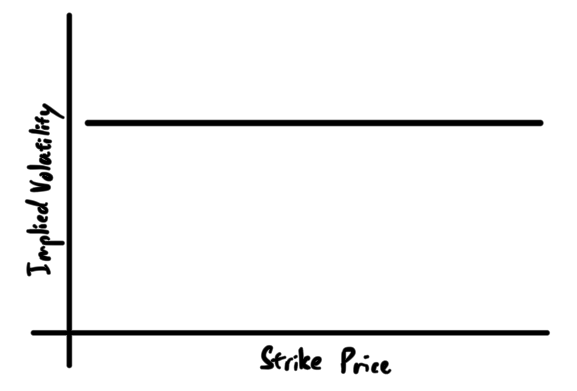
\includegraphics[scale=0.4]{img/expected_vol_graph.png}
      \caption{What we expect our strike price vs implied volatility graph to look like for a collection of options. } 
      \label{fig:expected_volatility_graph}
    \end{figure}

    \begin{definition}[Volatility Smile]
      Empirically, this is not the case, and we see a \textbf{volatility smile} centered around ATM. This means that ATM options have lower implied volatility than OTM or ITM options. Therefore, as the strike price moves away from the current stock price, the price of the options are in fact higher than what is accounted for in the Black-Scholes model, meaning that they are overvalued.  
      \begin{figure}[H]
        \centering 
        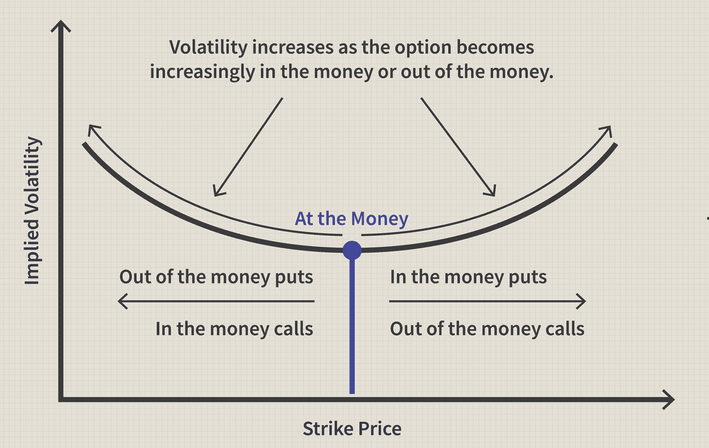
\includegraphics[scale=0.4]{img/vol_smile.png}
        \caption{Volatility smile} 
        \label{fig:vol_smile}
      \end{figure}
    \end{definition}

    However, this may not be symmetrical. 

    \begin{definition}[Volatility Skew/Smirk]
      
    \end{definition}

\section{Risk Measurement}

  \subsection{Delta}

    \begin{definition}[Delta]
      The \textbf{delta} of an option is defined 
      \begin{equation}
        \Delta_t \coloneqq \frac{\partial V_K (t, T)}{\partial S_t}
      \end{equation}
      meaning that for every \$1 increase in stock price, the option price increases roughly by \$$\Delta$, with all else being equal. It indicates how many options contracts are needed to hedge a long or short position in the underlying asset. Note that the delta for a call must be in $[0, 1]$ and of a put must be in $[-1, 0]$, but traders tend to describe it in $[0, 100]$ and $[-100, 0]$. 
      
      \begin{center}
%        \includegraphics[scale=0.3]{img/}
      \end{center}
    \end{definition}

    \begin{theorem}[Delta as Probability of ITM]
      A third, often useful, interpretation is that it is the \textit{approximate} (not exact) probability of the option finishing ITM. 
    \end{theorem}
    \begin{proof}
      TBD. 
    \end{proof}

    \begin{theorem}[Black Scholes]
      Given the BS formula, we have 
      \begin{align}
        \text{Call } \Delta_t & = \frac{\partial C_t}{\partial S_t} = \Phi(d_1) \\
        \text{Put } \Delta_t & = \frac{\partial P_t}{\partial S_t} = 1 - \Phi(d_1) \\
      \end{align}
      Therefore, we can interpret the first CDF term as the probability that the call delta finishes ITM. 
    \end{theorem}

    \begin{theorem}[Delta Effects with Volatility]
      As $\sigma \rightarrow +\infty$ for both ITM and OTM calls and puts, their $\Delta \rightarrow +\infty$. This makes sense because the probability of finishing either ITM or OTM is equal. As $\sigma \rightarrow 0$, 
      \begin{enumerate}
        \item ITM calls: $\Delta \rightarrow +100$. 
        \item ITM puts: $\Delta \rightarrow -100$. 
        \item OTM calls/puts: $\Delta \rightarrow 0$. 
      \end{enumerate}
    \end{theorem}

    \begin{theorem}[Delta Effects with Time]

    \end{theorem}

    \begin{theorem}[Delta Effects with Interest Rate]

    \end{theorem}

    \begin{definition}[Delta Hedging]
      \textbf{Delta hedging} is the process of dynamically hedging the option position with the underlying stocks. Given the nonlinearity, the hedge ratio has to be adjusted dynamically. For example, to hedge a short call option, we need to buy $\Delta$ amount for stock for each option. The resulting portfolio 
      \begin{equation}
        V_t = -C_t + \Delta S_t
      \end{equation}
      has the first derivative $0$, which is called \textbf{delta neutral}. However, as $S_t$ changes, the $\Delta_t$ changes by the amount of $\Gamma_T \Delta_t S_t$. That means 
      \begin{enumerate}
        \item when the price goes up, we need to buy more shares, and 
        \item when the prices goes down, we need to sell more shares. 
      \end{enumerate}
    \end{definition}

    If we perform delta hedging strategy continuously, we would have 
    \begin{equation}
      \text{PnL} = \int_0^T \frac{S_t^2}{2} \Gamma_t (\sigma_{\text{implied}}^2 - \sigma_{\text{realized}}^2 )\, dt
    \end{equation}

  \subsection{Gamma}

    \begin{definition}[Gamma]
      The \textbf{gamma} is the sensitivity of $\Delta$ w.r.t. $S$, i.e. the double derivative. 
      \begin{equation}
        \Gamma_t \coloneqq \frac{\partial^2 V_K (t, T)}{\partial S_t^2}
      \end{equation}
    \end{definition}

    \textbf{Gamma scalping.}

    \begin{theorem}[Delta and Gammas as Time Passes]
      
    \end{theorem}

    \begin{theorem}
      \begin{equation}
        \Gamma_t = \frac{\partial^2 C_t}{\partial S_t^2} = \frac{\partial^2 P_t}{\partial S_t^2} = \frac{1}{S_0 \sigma \sqrt{T - t}} \frac{1}{\sqrt{2\pi}} e^{- d_1^2 / 2} \\
      \end{equation}
    \end{theorem}

  \subsection{Theta}

    \begin{definition}[Theta]
      The \textbf{theta} measures the impact of a change in time remaining. 
      \begin{equation}
        \Theta_t \coloneqq \frac{\partial V_t}{\partial t}
      \end{equation}
    \end{definition}

  \subsection{Vega}

    \begin{definition}[Vega]
      The \textbf{vega} measures the impact of a change in the volatility of the underlying. 
      \begin{equation}
        \nu_t \coloneqq \frac{\partial V_K (t, T)}{\partial \sigma}
      \end{equation}
    \end{definition}

    \begin{theorem}[Properties]
      Given the Black-Scholes model, we can derive the following formulas: 
      \begin{align*}
        \nu_t & = \frac{\partial C_t}{\partial \sigma} = \frac{\partial P_t}{\partial \sigma} = S_0 \sigma \sqrt{T - t} \frac{1}{\sqrt{2\pi}} e^{-d_1^2 / 2} = \sigma^2 (T - t) \Gamma_t 
      \end{align*}
    \end{theorem}

  \subsection{Rho}

    \begin{definition}[Rho]
      The \textbf{rho} measures the impact of a change in interest rates. 
      \begin{equation}
        \rho_t \coloneqq \frac{V_K (t, T)}{\partial r}
      \end{equation}
    \end{definition}

\end{document}
